% Group addresses by affiliation; use superscriptaddress for long
% author lists, or if there are many overlapping affiliations.
% For Phys. Rev. appearance, change preprint to twocolumn.
% Choose pra, prb, prc, prd, pre, prl, prstab, prstper, or rmp for journal
%  Add 'draft' option to mark overfull boxes with black boxes
%  Add 'showpacs' option to make PACS codes appear
%  Add 'showkeys' option to make keywords appear
\listfiles
\documentclass[aps,
prd,
amsmath,
amssymb,
twocolumn,
%preprint,
floatfix,
groupedaddress]{revtex4-1}
%\documentclass[aps,prl,preprint,superscriptaddress]{revtex4-1}
%\documentclass[aps,prl,reprint,groupedaddress]{revtex4-1}
\usepackage[pdftex]{graphicx}% Include figure files
%\usepackage{float}
%\usepackage{stfloats}
%\usepackage{fixltx2e}
\usepackage{placeins}
\usepackage{dcolumn}% Align table columns on decimal point
%\usepackage{amsmath}
\usepackage{amsthm, amsfonts, amssymb}
%\usepackage{supertabular}
\usepackage{array}
\usepackage{times}
\usepackage{latexsym}
\usepackage{hyperref}
\hypersetup{backref,  
%pdfpagemode=FullScreen,  
colorlinks=true,
linkcolor=red,
filecolor=red,
citecolor=blue}
\usepackage{epsfig}
\usepackage{subfigure}
% \usepackage{multicol}
%\usepackage{acronym}
%\usepackage[caption=false]{caption}
\usepackage{bm}% bold math
\usepackage{color}

\newcommand{\Sum}{\displaystyle\sum\limits}
\newcommand{\Int}{\displaystyle\int\limits}
\newcommand{\ii}{{\rm i}}
\newcommand{\D}{\mathrm{d}}
\newcommand{\eff}{\mathrm{eff}}
\newcommand{\phys}{\mathrm{phys}}
\newcommand{\real}{\mathrm{real}}
\newcommand{\peak}{\mathrm{peak}}
\newcommand{\EOB}{\mathrm{EOB}}
\newcommand{\NR}{\mathrm{NR}}
\newcommand{\RD}{\mathrm{RD}}
\newcommand{\Olap}{\mathcal{O}}
\newcommand{\FF}{\mathcal{FF}}
\newcommand{\MM}{\mathrm{MM}}
\newcommand{\EFF}{\mathrm{EFF}}
\newcommand{\X}{\mathrm{X}}
\newcommand{\Y}{\mathrm{Y}}
\newcommand{\Z}{\mathrm{Z}}
\newcommand{\horizon}{\mathrm{Horizon}}
\newcommand{\opt}{\mathrm{opt}}
\newcommand{\iso}{\mathrm{iso}}
\newcommand{\refr}{\mathrm{ref}}
\newcommand{\start}{\mathrm{start}}

\def\l({\left(}
\def\r){\right)}
%\def\l[{\left[}
%\def\r]{\right]}

\def\beq{\begin{equation}}
\def\eeq{\end{equation}}
\def\bea{\begin{eqnarray}}
\def\eea{\end{eqnarray}}
\def\nn{\nonumber}
\def\del{\partial}
\def\ola{\overleftarrow}
\def\ora{\overrightarrow}

% You should use BibTeX and apsrev.bst for references
% Choosing a journal automatically selects the correct APS
% BibTeX style file (bst file), so only uncomment the line
% below if necessary.
%\bibliographystyle{apsrev4-1}

\begin{document}

% Use the \preprint command to place your local institutional report
% number in the upper righthand corner of the title page in preprint mode.
% Multiple \preprint commands are allowed.
% Use the 'preprintnumbers' class option to override journal defaults
% to display numbers if necessary
%\preprint{}

%Title of paper
\title{Effectualness of Effective One Body Templates in Advanced LIGO}

% repeat the \author .. \affiliation  etc. as needed
% \email, \thanks, \homepage, \altaffiliation all apply to the current
% author. Explanatory text should go in the []'s, actual e-mail
% address or url should go in the {}'s for \email and \homepage.
% Please use the appropriate macro foreach each type of information

% \affiliation command applies to all authors since the last
% \affiliation command. The \affiliation command should follow the
% other information
% \affiliation can be followed by \email, \homepage, \thanks as well.
\author{Duncan A. Brown}
%\email[]{dabrown@physics.syr.edu}
%\homepage[]{Your web page}
%\thanks{}
%\altaffiliation{}
\affiliation{Department of Physics, Syracuse University, Syracuse, NY 13244}

\author{Prayush Kumar}
%\email[]{prkumar@syr.edu}
%\homepage[]{Your web page}
%\thanks{}
%\altaffiliation{}
\affiliation{Department of Physics, Syracuse University, Syracuse, NY 13244}

\author{Alexander H. Nitz}
%\email[]{ahnitz@syr.edu}
%\homepage[]{Your web page}
%\thanks{}
%\altaffiliation{}
\affiliation{Department of Physics, Syracuse University, Syracuse, NY 13244}

%Collaboration name if desired (requires use of superscriptaddress
%option in \documentclass). \noaffiliation is required (may also be
%used with the \author command).
%\collaboration can be followed by \email, \homepage, \thanks as well.
%\collaboration{}
%\noaffiliation

%\date{\today}

\begin{abstract}
Coalescing stellar-mass binary black holes (BBHs) are likely sources of
gravitational waves for the Laser Interferometer Gravitational-wave
Observatory (LIGO) and the Virgo gravitational-wave observatory.  Optimal
searches for BBHs require template banks of signal waveforms that accurately
covers the parameter space of possible sources.  Sufficient accuracy is
usually defined as an event rate loss of no less than $\sim 10\%$ due to the
discrete nature of the template bank and errors in the waveforms.  A new
Effective One Body (EOB) model (EOBNRv2) has recently been calibrated against
full numerical binary black-hole merger simulations and is believed to provide an
accurate waveform model for searches in the the second-generation detectors
Advanced LIGO and Advanced Virgo. In this paper, we investigate three items of
importance to advanced-detector BBH searches: First, we study the accuracy
of the currently available second-order post-Newtonian, hexagonal template
placement metric for BBH searches which use EOBNRv2 waveforms.  We find that
the existing algorithm works well for BBHs with component masses in the range $3
M_\odot \le m_1, m_2 \le 25\, M_\odot$.  For a template bank constructed with
a minimal match of $97\%$ less than $1.5\%$ of non-spinning BBH signals have a
mismatch greater than $3\%$.  Second, we investigate the mass range in which
the (computationally less expensive) TaylorF2 post-Newtonian waveforms can be
used, and where full EOBNRv2 waveforms are required. We find that for
non-spinning BBHs with $M \lesssim 8.8\,M_{\odot} (14\,M_{\odot})$, a TaylorF2
detection search is viable with a loss of no more than $10\%\, (15\%)$ in the
event rate.  Finally, we investigate the effect of modes other than the
dominant $l = m = 2$ mode in BBH searches.  If we assume that BBH signals are
accurately modeled by the EOBNRv2 waveform including the five leading modes,
we find that for systems with $(m_1/m_2)\leq 1.5$, there is no significant loss
in the total possible signal-to-noise ratio due to neglecting modes greater
than $l = m = 2$ in the template waveforms. For higher mass ratios, including
higher order modes could increase the signal-to-noise ratio by as much as
$8\%$ in Advanced LIGO. 
\end{abstract}

% insert suggested PACS numbers in braces on next line
\pacs{}
% insert suggested keywords - APS authors don't need to do this
%\keywords{}

%\maketitle must follow title, authors, abstract, \pacs, and \keywords
\maketitle

\section{Introduction}\label{sec:level1:Introduction}
In the last several decades, there has been tremendous progress towards the
first direct detection of gravitational waves (GWs). Upgrades to the Laser
Interferometer Gravitational-Wave Observatory (LIGO) are currently underway,
with completion scheduled for 2014. Similar upgrades are scheduled for the
Virgo gravitational-wave detector. When the Advanced LIGO (aLIGO) detectors
reach design sensitivity in $\sim 2018$, they will have a factor of a
thousandfold increase in the observable volume of space
\citep{aLIGOsensitivity}, compared to the first-generation detectors.

The inspiral and merger of stellar-mass binary black holes (BBHs), with component masses between $3 \, M_{\odot} \lesssim m_1, m_2 \lesssim 25 M_{\odot}$, are expected to be an important class of candidate events
for detection by aLIGO \citep{300yrsofGravitation}. aLIGO will be able to
detect GW signals from BBH systems with component masses $m_1 = m_2 = 25 \,
M_{\odot}$ to a maximum distance of up to $\sim 3.6$~Gpc. The rate of BBH
coalescences that will be observed by aLIGO is estimated to be
between $0.2\,\mathrm{yr}^{-1}$ and $1000\,\mathrm{yr}^{-1}$
\citep{LSCCBCRates2010}.
Accurate knowledge of the GW signals generated by BBHs is crucial for
detecting and understanding these sources. Past searches for GWs from BBHs
\citep{Colaboration:2011nz,Abadie:2010yb,Abbott:2009qj,Abbott:2009tt,Messaritaki:2005wv} used matched-filtering
\citep{Wainstein:1962,Allen:2005fk} to correlate detector data against a template bank of
analytically modeled waveforms which cover the search parameter space. This
technique is sensitive to the accuracy of the waveform templates that are used
as filters \citep{FittingFactorApostolatos}. If the model used to construct
search templates does not accurately reproduce the true signals, the
sensitivity of detection searches is reduced
\citep{WaveformAccuracy2008,WaveformAccuracy2010}. Optimal searches therefore
require an accurate waveform model.

The dynamics of a BBH system can been modeled in three regimes: (i) The early inspiral, when the separation between the black holes is large, can be modeled using results from post-Newtonian (PN) theory \citep{PNtheoryLivingReviewBlanchet}. The PN expressions for the gravitational-wave phase of non-spinning binaries are available up to 3.5PN order \citep{PNFluxEnergy3PN01,PNFluxEnergy3PN02,Jaranowski:1999qd,Jaranowski:1999ye,Damour:2001bu,KidderPN,Blanchet3PN}. (ii) Insight into the late-inspiral and merger phase has been provided by numerical solutions of the Einstein equations \citep{Pretorius2005,Pretorius2006,BBHNRScheel,BBHNRGonzalezq10,BBHNRPollney,BBHNRLoustoq10,Buchman:2012dw}. These simulations are computationally expensive, and so are only available for a relatively small number of binary systems, see e.g. \citep{Ajith:2012tt}. The analytic Effective-One-Body (EOB) approach \citep{EOBOriginalBuonannoDamour} has been proposed to model the inspiral-merger phase and has been tuned to Numerical 
Relativity (NR) simulations in this regime \citep{EOBNR01,EOBNRdevel01,EOBNRdevel02,EOBNRdevel03,EOBNRdevel04,EOBdevel01,EOBdevel02,BuonannoEOBv2Main}. (iii) The ringdown phase is modeled using a super-position of quasi-normal modes (QNMs) which describe the oscillations of the Kerr black-hole that is formed from the coalescence \citep{BHRDQNMs,BHPTMinoSasaki}. A new EOB waveform family (called EOBNRv2) has been proposed that incorporates information from several non-spinning BBH NR simulations, with QNMs attached to provide a complete BBH waveform \citep{BuonannoEOBv2Main}. This waveform is believed to be sufficiently accurate to search for non-spinning BBH signals in the aLIGO sensitive band (10-1000 Hz).

Detection searches for GWs from BBHs must search for all possible combination of the binary's component masses within the mass parameter space of interest. This is performed by constructing a \textit{bank} of template waveforms which covers the range of BBH component masses \citep{Sathyaprakash:1991mt,Balasubramanian:1995bm}. Search template banks are constructed such that no more than a pre-specified fraction of the total events are lost due to the discrete nature of the grid. The coverage of the template bank is specified by the \textit{minimal match} ($\MM$). The minimal match quantifies the loss in signal-to-noise ratio caused by the discrete nature of the template bank \citep{FittingFactorApostolatos}. For example, a bank with a minimal match of $0.97$ would lose no more than $3\%$ of the maximum possible signal-to-noise ratio (SNR) due to differences between the nearest closest template waveform and an arbitrary waveform in the from the space of the template bank. The template bank placement metric 
used in previous LIGO-Virgo BBH searches is constructed using the 2PN accurate Taylor F2 PN waveforms for binary neutron stars \citep{OwenTemplateSpacing,SathyaBankPlacementTauN,BabaketalBankPlacement,SathyaMetric2PN}, and its validity for placing a bank of EOB waveforms is not \textit{a priori} guaranteed. We investigate the accuracy of this metric for constructing a bank of templates to search for non-spinning stellar mass BBHs using EOBNRv2 waveforms in aLIGO. We construct a template bank of EOBNRv2 waveforms with $\MM$ of $0.97$, and calculate its fitting factor ($\FF$) against $\sim 90,000$ simulated EOBNRv2 signals with component masses uniformly distributed between $3 M_{\odot} \le m_1,m_2 \le 25 M_{\odot}$. We find that the $\FF$ of the template bank is greater than $0.97$ for $98.5\%$ of the simulated EOBNRv2 signals, assuming the Zero-Detuned High Power noise spectrum for aLIGO sensitivity \citep{aLIGONoiseCurve}. We conclude that the existing placement algorithm is sufficient for use in aLIGO BBH 
searches, if EOBNRv2 is an accurate model of BBH signals.

Previous searches for stellar-mass BBHs  with total mass $M \lesssim 25 M_\odot$ in LIGO and Virgo used the restricted TaylorF2 PN waveforms  \citep{Sathyaprakash:1991mt,Cutler:1994ys,Droz:1999qx}. Since this waveform is analytically generated in the frequency domain, it is less computationally expensive than EOB templates when used for matched filtering. However, use of the TaylorF2 waveform may result in a loss in search efficiency due to inaccuracies of the PN approximation for BBHs. Earlier studies using the EOBNRv1 model \citep{Buonanno:2007pf,Buonanno:2002ft} have estimated that detection searches can use Taylor F2 templates for BBHs with total mass below $12M_{\odot}$ \citep{CompTemplates2009}. We revisit this question using the restricted Taylor F2 waveforms for aLIGO BBH searches. To estimate the range of BBH systems for which Taylor F2 template banks can be used in aLIGO detection searches, we impose the accuracy criterion that the loss in detection rate due to waveform inaccuracy and bank 
discreteness should be less than $10\%\, ($or $15\%)$. This criterion is equivalent to the $\FF$ of the bank not falling below $0.965\, ($or $0.947)$. To model the \textit{true} GW signals, we use the EOB model of Ref.~\citep{BuonannoEOBv2Main} which includes the first five waveform multipoles (EOBNRv2HM). We find that a $0.97\MM$ template bank of 3.5PN restricted Taylor F2 waveforms can be used to search for BBH systems with total mass is less than $8.8M_{\odot}\, (14M_{\odot})$.

Finally, we investigate the loss in the SNR incurred by the using template banks constructed using only the leading order mode of EOBNRv2 waveforms. Current GW searches only use the dominant $l=m=2$ mode in their waveform templates. We model the true GW signals using EOBNRv2HM waveforms and calculate the $\FF$ of the EOBNRv2 template bank for $\sim 100,000$ simulated BBHs. We find that a template bank constructed with a $\MM$ of $0.97$ can be used to search for BBHs for which $1\leq \l(m_1/m_2\r)\leq 1.5\, (3.25)$ with less than $10\%\, (15\%)$ loss in detection rate. For such systems, using EOBNRv2HM templates is unlikely to give a significant increase in the range to which they can be detected. For BBH with $\l(m_1/m_2\r)\geq 1.5\, (3.25)$, detection searches could possibly gain sensitivity by the use of EOBNRv2HM waveforms. This is further illustrated in Fig.~\ref{fig:RatioOfRangesHM22}, where we show the ratio of the sensitivity range that we have available to us when we use EOBNRv2HM templates to that 
which is available when we use EOBNRv2 templates.

The remainder of this paper is organized as follows: Sec.~\ref{sec:level1:WaveformApproximants} reviews the Taylor F2 (Sec.~\ref{sec:level2:TaylorF2}) and EOBNRv2(HM) (Sec.~\ref{sec:level2:EOBNRv2}) waveforms that are used in our study. In the beginning of Sec.~\ref{sec:level1:FFStudy}, we describe the fitting-factor $\FF$ that we use to evaluate the performance of the template banks. In Sec.~\ref{sec:level2:EOBNRv2templateplacement} we present the results of the Monte-Carlo study where we study the efficiency of the existing 2PN hexagonal bank placement metric in placing a template bank of EOBNRv2 waveforms. Sec.~\ref{sec:level2:EffectualnessTaylorF2} shows the results of the Monte-Carlo study to determine the region of the BBH component-mass space where detection searches can use 3.5PN Taylor F2 waveform template bank. Sec.~\ref{sec:level2:EffectualnessEOBNRv2} illustrates the effect of excluding higher order modes in the signal waveforms in an EOBNRv2 search. The main conclusions of the study are 
presented in Sec.~\ref{sec:level1:conclusion}.


\section{Waveform Approximants}\label{sec:level1:WaveformApproximants}
In this section we review the construction of the restricted TaylorF2 and EOBNRv2 waveforms used in this study. Throughout, we set $G=c=1$.
\subsection{Taylor F2}\label{sec:level2:TaylorF2}
In this section, we present the basic equations that describe the construction of the restricted TaylorF2 waveform. In the adiabatic approximation, we can visualize the course of inspiral as a series of radially shrinking circular orbits. 
The radial coordinate evolves as the binary loses energy to gravitational radiation that propagates outwards from the system.
For a binary with individual component masses $m_1$ and $m_2$ and total mass $M=m_1+m_2$, the conserved energy accurate to 3PN
can be written as \citep{Jaranowski:1997ky,Jaranowski:1999ye,Jaranowski:1999qd,Damour:2001bu,Blanchet:2003gy,Damour:2000ni,Blanchet:2002mb}
\begin{equation}
\begin{split}\label{eq:E3PN}
E_3(v)=&-\dfrac{1}{2}\eta v^2 \left[1- \l(\dfrac{3}{4}+\dfrac{1}{12}\eta\r)v^2 - \l(\dfrac{27}{8}-\dfrac{19}{8}\eta\right.\right.\\
+&\left.\left.\dfrac{1}{24}\eta^2 \r)v^4 - \l(\dfrac{675}{64}-\l(\dfrac{34445}{576}-\dfrac{205}{96}\pi^2\r)\eta\right.\right.\\
+&\left.\left.\dfrac{155}{96}\eta^2 +\dfrac{35}{5184}\eta^3\r) v^6\right],
\end{split}
\end{equation}
where $\eta=m_1m_2/(m_1+m_2)^2$, $v=(\pi Mf)^{1/3}$ is the characteristic velocity of the binary, and $f$ denotes the frequency of the emitted gravitational wave throughout.
The gravitational flux from such a system, accurate to 3.5PN is given by \citep{FluxandE3-5PN,Blanchet:2004ek,Blanchet:2005tk,Blanchet:2004bb}
\begin{equation}
\begin{split}\label{eq:Ft3.5PN}
F_{3.5}(v)=&\dfrac{32}{5}\eta^2 v^{10}\left[1 - \l(\dfrac{1247}{336}+\dfrac{35}{12}\eta\r)v^2+4\pi v^3\right.\\
-&\left.\l(\dfrac{44711}{9072}-\dfrac{9271}{504}\eta -\dfrac{65}{18}\eta^2 \r)v^4\right.\\
-&\left.\l(\dfrac{8191}{672}+\dfrac{583}{24}\eta\r)\pi v^5+ \l(\dfrac{6643739519}{69854400}\right.\right.\\
+&\left.\left.\dfrac{16}{3}\pi^2 -\dfrac{1712}{105}\gamma +\l(\dfrac{41}{48}\pi^2 -\dfrac{134543}{7776}\r)\eta \right.\right.\\
-&\left.\left.\dfrac{94403}{3024}\eta^2 -\dfrac{775}{324}\eta^3 -\dfrac{856}{105}\textrm{log}(16v^2)\r)v^6\right.\\ 
-&\left.\l(\dfrac{16285}{504}-\dfrac{214745}{1728}\eta -\dfrac{193385}{3024}\eta^2 \r)\pi v^7\right],
\end{split}
\end{equation}
where $\gamma$ is Euler's constant.
%In the limit $\dot{\omega}/\omega \ll 1$, we can approximate the energy of the system to be the energy averaged over a period. Combining the energy balance equation, $\D E(v)/\D t = -F(v)$, with Kepler's law gives a system of coupled differential equations for the evolution of the orbital phase,
%\begin{subequations}\label{eq:PNOrbitalEvolution01}
%\begin{align}
%\dfrac{\D\phi}{\D t} - \dfrac{v^3}{M} &= 0,\label{eq:PNOrbitalEvolution01_01}\\
%\dfrac{\D v}{\D t} + \dfrac{F(v)}{M\l(\D E/\D v\r)} &= 0.\label{eq:PNOrbitalEvolution01_02}
%\end{align}
%\end{subequations}
%We can rewrite these eqs. in integral form as follows,
%\begin{subequations}\label{eq:PNOrbitalEvolution02}
%\begin{align}
%t(v) &= t_{\refr} + M\Int_v^{v_{\refr}}\D v\dfrac{E^{\prime}(v)}{F(v)},\label{eq:PNOrbitalEvolution02_01}\\
%\phi(v) &= \phi_{\refr} + \Int_v^{v_{\refr}}\D v\,v^3\dfrac{E^{\prime}}{F(v)};\label{eq:PNOrbitalEvolution02_02}
%\end{align}
%\end{subequations}
%where $t_{\refr}$ and $\phi_{\refr}$ are integration constants and $v_{\refr}$ is an arbitrary reference velocity.
%We can use these constants to set the appropriate initial conditions for the generation of the inspiral.
%\subsection{Taylor T1}\label{sec:level3:Waveform:T1}
%If we substitute the expressions for the Energy of and flux from a particular system, exactly as they are from Eq.~\eqref{eq:E3PN},~\eqref{eq:Ft3.5PN} into Eq.~\eqref{eq:PNOrbitalEvolution01}, and numerically solve it, the phase evolution thus obtained gives us the T1 waveform.
%
%Truncating the expression for Energy and flux at $n$PN order\citep{FluxandE3-5PN,PNFluxEnergy2PN,PNFluxEnergy3PN01,PNFluxEnergy3PN02}, results in a $n$PN template model\citep{CompTemplates2001,GW2PN}.
%
%The initial conditions for the inspiral are specified in terms of a particular starting gravitational wave frequency ($f_{start}$). This is incorporated by putting:
%\begin{align*}
%t_{ref} &= 0\\
%v_{ref} &= (\pi M f_{start})^{1/3}\\
%\phi_{ref} &= 0 \texttt{or} \pi/2
%\end{align*}
%
%giving us a pair of orthogonal templates, one corresponding to each value of $\phi_{ref}$.

%\subsubsection{Taylor T3}\label{sec:level2:TaylorT3}
%We start with explicitly inverting Eq.~\eqref{eq:PNOrbitalEvolution02_01} to obtain $v(t)$, as a function of
%\begin{equation}
% \Theta = \l(\dfrac{v(t_{\refr}-t)}{5M}\r)^{-1/8}.
%\end{equation}
%From $v(t)$, we get $f(t)\equiv v(t)^3/(\pi M)$, which is the gravitational wave frequency at any instant of time during the course of the inspiral.
%The expression for $v(t)$ can be substituted in Eq.~\eqref{eq:PNOrbitalEvolution02_02} to obtain $\phi(t)$. After this series of operations,
%we obtain the Taylor T3 gravitational phase and frequency as a function of time,
%\begin{subequations}
%\begin{align}
%\phi^{(T3)}_n(t) &= \phi^{(T3)}_{\refr} + \phi^t_n\Sum^{2n}_{k=0}C^{\phi}_k \Theta^k,\\
%f^{(T3)}_n(t) &= f^t_n\Sum^{2n}_{k=0}C^f_k \Theta^k,\label{eq:T3frequency}
%\end{align}
%\end{subequations}
%where $C^{\phi}_k$, $C^f_k$, $\phi^t_n$ and $f^t_N$ are constants,
%and the subscript $n$ stands for the post-Newtonian order to which the respective expression is accurate.
%Complete expressions for $\phi^{(T3)}_n(t)$ and $f^{(T3)}_n(t)$ can be obtained from Ref.~\citep{CompTemplates2009}.
%To setup the initial conditions, one can solve Eq.~\eqref{eq:T3frequency} for $t_{\refr}$, such that\newline
%$f^{(T3)}_n(0)=f_{\start}$.

%\subsubsection{Taylor T4}\label{sec:level2:TaylorT4}
%This approximant was originally proposed in Ref.~\citep{TaylorT4Origin} and developed subsequently \citep{NRPNComparisonBaker2007,NRdynamicsq1,NRPNComparisonBoyleetal}.
%We substitute the expression for energy from Eq.~\eqref{eq:E3PN}, and the expression for flux from Eq.~\eqref{eq:Ft3.5PN} into Eq.~\eqref{eq:PNOrbitalEvolution01_02},
%and expand $F(v)/ME^{\prime}(v)$ upto consistent PN order \citep{FluxandE3-5PN,PNFluxEnergy2PN,PNFluxEnergy3PN01,PNFluxEnergy3PN02,CompTemplates2001,GW2PN}.
%The Eqns.~\eqref{eq:PNOrbitalEvolution01} can subsequently be numerically solved to obtain the phase and gravitational-wave frequency as functions of time.
%Thus we obtain the Taylor T4 phase evolution. The initial conditions for the inspiral are specified in terms of a particular starting gravitational-wave
%frequency ($f_{\start}$). This is incorporated by putting
%\begin{subequations}
%\begin{align}
%t_{\refr} &= 0,\\
%v_{\refr} &= (\pi M f_{\start})^{1/3},\\
%\phi_{\refr} &= 0\quad \textit{or}\quad \pi/2;
%\end{align}
%\end{subequations}
%giving us a pair of orthogonal templates, one corresponding to either value of $\phi_{\refr}$.
Using the stationary phase approximation \citep{MatthewsWalker}, the gravitational waveform in the Fourier domain can be approximated as \citep{Cutler:1994ys,Droz:1999qx}
\begin{subequations}
\begin{align}
\tilde{h}(f) &= \dfrac{a(t(f))}{\sqrt{\dot{f}(t(f))}}e^{\ii \l(\Psi_f(t(f)) - \pi/4\r)},\\
\Psi_f(t) &\equiv 2\pi ft - 2\phi(t)\label{eq:PsiFofPhi};
\end{align}
\end{subequations}
where $t(f)$ is the time at which the instantaneous gravitational wave frequency of the binary is equal to $f$, the Fourier frequency. In the adiabatic approximation, $t(f)$ and $\Psi_f$ can be obtained from
\begin{subequations}
\begin{align}\label{eq:PNF2Evolution01}
\dfrac{\D\Psi}{\D f}-2\pi t &= 0,\\
\dfrac{\D t}{\D f} + \dfrac{\pi M^2}{3v^2}\dfrac{E^{\prime}(v)}{F(v)} &=0;
\end{align}
\end{subequations}
which come from Eq.~\eqref{eq:PsiFofPhi} and the energy balance relation $\D E(v)/\D t = -F(v)$. The Taylor F2 waveform $\tilde{h}(f)$ can be written  directly in the frequency domain as
\begin{equation}
\tilde{h}(f) = Af^{-7/6}e^{\iota\Psi(f)},
\end{equation}
where we have kept only the leading-order amplitude terms; this is known as the restricted PN waveform. The amplitude $A\propto (m_1+m_2)^{5/6}\eta^{1/2}/\mathcal{R}$, where $\mathcal{R}$ is the distance to the binary. The Fourier phase of the waveform at 3.5PN order is given by \citep{Sathyaprakash:1991mt,Cutler:1994ys,GW2PN,Blanchet:2001ax,Blanchet:2004ek,Poisson:1995ef,Allen:2005fk}
\begin{equation}
\begin{split}\label{eq:PsiSPA}
\Psi(f)=&2\pi ft_c-\phi_c-\dfrac{\pi}{4} + \dfrac{3}{128}\dfrac{1}{\eta}v^{-5}\left[1 + \l(\dfrac{3715}{756} +\dfrac{55}{9}\eta\r)v^2\right.\\
-&\left. 16\pi v^3+\l(\dfrac{15293365}{508032}+\dfrac{27145}{504}\eta +\dfrac{3085}{72}\eta^2 \r)v^4\right.\\
+&\left.\l(\dfrac{38645}{756}-\dfrac{65}{9}\eta\r)\l(1+3\textrm{log}\l(\dfrac{v}{v_{\textrm{lso}}}\r)\r)\pi v^5\right.\\
+&\left.\left[\dfrac{11583231236531}{4694215680}-\dfrac{640}{3}\pi^2 -\dfrac{6848}{21}\gamma_E\right.\right.\\
-&\left.\left. \dfrac{6828}{21}\textrm{log}(4v)+\l(-\dfrac{15737765635}{3048192}+\dfrac{2255}{12}\pi^2 \r)\eta\right.\right.\\
+&\left.\left.\dfrac{76055}{1728}\eta^2 -\dfrac{127825}{1296}\eta^3\right] v^6\right.\\
+&\left.\l(\dfrac{77096675}{254016}+\dfrac{378515}{1512}\eta -\dfrac{74045}{756}\eta^2 \r)\pi v^7\right].
\end{split}
\end{equation}
The initial conditions are set by starting the waveform from a given gravitational-wave frequency $f=f_{\mathrm{low}}$.

\subsection{Effective-One-Body Approximant}\label{sec:level2:EOBNRv2}
The dynamics of a two-body system can be mapped onto an effective-mass moving in a deformed Schwarzschild-like background, and is accomplished by the EOB approach \citep{EOBOriginalBuonannoDamour}. With the recent advancements in NR, the EOB model can now be tested and calibrated against numerical simulations of BBHs \cite{EOBdevel01,EOBdevel02,EOBNRdevel03,DamourFluxhlm01,EOBNRdevel01}. The EOB model proposed recently in Ref.~\citep{BuonannoEOBv2Main} has been calibrated to NR waveforms for binaries of mass-ratios $q=\{1,2,3,4,6\}$, where $q\,\equiv \, m_1/m_2$. In this section we summarize the essential features of the model. 

\subsubsection{The Hamiltonian}\label{sec:level3:EOBNRv2:Hamiltonian}
%\textcolor{green}{Describe the effective and real hamiltonians. Describe the tuned parameters in the metric.}
The EOB approach maps the fully general-relativistic dynamics of the two-body system to that of an \textit{effective} mass moving in a deformed Schwarzschild spacetime \citep{EOBOriginalBuonannoDamour}. The physical dynamics is contained in the deformed-spacetime's metric coefficients, the EOB Hamiltonian \cite{EOBOriginalBuonannoDamour}, and the radiation-reaction force. In polar coordinates $(r,\Phi)$, the EOB metric is written as
\begin{equation}\label{eq:dsEOB}
\D s_{\eff}^2 = -A(r)\D t^2 + \dfrac{A(r)}{D(r)}\D r^2 + r^2\left(\D\Theta^2 + \sin^2\Theta \D\Phi^2\right).
\end{equation}
The geodesic dynamics of the \textit{effective} mass $\mu\,=\,m_1 m_2 / M$ in the background of Eq.~\eqref{eq:dsEOB} is described by the Hamiltonian $H^{\eff}$, which can be written as \citep{EOBOriginalBuonannoDamour,PadeAD}
\begin{equation}
\begin{split}
H^{\eff} =\, & \mu\hat{H}^{\eff} \\
         =\, & \mu\sqrt{A(r) \left( 1 +  \dfrac{A(r)}{D(r)}p_r^2 + 2(4 - 3\eta)\eta \dfrac{p_r^4}{r^2} + \dfrac{p^2_{\Phi}}{r^2} \right)},
\end{split}
\end{equation}
where $(p_r,p_{\Phi})$ are momenta conjugate to $(r,\Phi)$ respectively. It was found convenient to replace the radial momentum $p_r$, with the momentum conjugate to the EOB extension of the Regge-Wheeler \textit{tortoise} radial coordinate $r_*$, where $r_*\equiv\int\sqrt{D(r)}/A(r)\,\D r$ \citep{DamourNQC01} . This momentum coordinate $p_{r_*}$ is related to $p_r$ as
\begin{equation}
p_{r_*} = \dfrac{A(r)}{\sqrt{D(r)}}\,p_r.
\end{equation}
In $\l(r,\Phi,p_{r_*},p_{\Phi}\r)$ coordinates, the effective Hamiltonian can be re-written as \citep{BuonannoEOBv2Main},
\begin{equation}
\hat{H}^{\eff} = \sqrt{p^2_{r_*} + A(r) \left( 1 + 2(4 - 3\eta)\eta \dfrac{p_{r_*}^4}{r^2} + \dfrac{p^2_{\Phi}}{r^2} \right)}.
\end{equation}
The EOB Hamiltonian (labeled the \textit{real} Hamiltonian), that describes the conservative dynamics of the binary,  is related to the effective Hamiltonian by the mapping
\begin{equation}
H^{\real} = \mu\hat{H}^{\real} = \mu\dfrac{1}{\eta} \sqrt{1 + 2\eta (\hat{H}^{\eff} - 1)}.
\end{equation}
The metric coefficients $A(r)$ and $D(r)$ were originally calculated as Taylor expansions \cite{EOBOriginalBuonannoDamour,PadeAD}, and to $n$-PN order they can be written as
\begin{eqnarray}
A(r) = \Sum^{n+1}_{i=0} \dfrac{a_i (\eta)}{r^i},\quad
D(r) = \Sum^{n}_{i=0} \dfrac{d_i (\eta)}{r^i};
\end{eqnarray}
where currently $A(r)$ and $D(r)$ are known to 3PN order $\l(n=3\r)$.  The EOBNRv2 model uses Pade-resummations of the Taylor expansions of these coefficients \citep{BuonannoEOBv2Main}. The use of re-summation techniques to express their Taylor expansions as ratios of polynomials was proposed to ensure the existence of the innermost stable circular orbit in the EOB framework \citep{PadeAD}. Their resummed expression are given by \citep{BuonannoEOBv2Main}
\begin{eqnarray*}
D(r) &=& \dfrac{r^3}{(52\eta - 6\eta^2) + 6\eta r + r^3},\\
A(r) &=& \dfrac{\alpha_0 r^5 + \alpha_1 r^4}{\beta_0 r^5 + \beta_1 r^4 + \beta_2 r^3 + \beta_3 r^2 + \beta_4 r +\beta_5};
\end{eqnarray*}
where,
\begin{equation}
\begin{split}
\alpha_0 &= 32 - 4a_4 - a_5 - 24\eta ,\\
\alpha_1 &= -64 + 12a_4 + 4a_5 + a_6 + 64\eta - 4\eta^2 ,\\
\beta_0 &= 32 - 4a_4 - a_5 - 24\eta ,\\
\beta_1 &= 4a_4 + 2a_5 + a_6 + 16\eta - 4\eta^2 ,\\
\beta_2 &= 8a_4 + 4a_5 + 2a_6 + 32\eta - 8\eta^2 ,\\
\beta_3 &= 16a_4 + 8a_5 + 4a_6 + \left(8a_4 + 2a_5\right)\eta + 32\eta^2 ,\\
\beta_4 &= 4a_4^2 + a_4a_5 + 16a_5 + 8a_6\\ 
             &+ \left(32a_4 - 2a_6\right)\eta + 32\eta^2 + 8\eta^3 ,\\
\beta_5 &= 4a_4^2 + 4a_4a_5 + a+5^2 - a_4a_6 + 16a_6\\
             &+ \left(32a_4 + 16a_5 - 8a_6\right)\eta + 4a_4\eta^2 + 32\eta^3 ,
\end{split}
\end{equation}
with
\begin{equation}\label{metric_a4}
a_4 = \left(\dfrac{94}{3} - \dfrac{41}{32}\pi^2\right)\eta.
\end{equation}
The 4PN and 5PN coefficients $a_5$ and $a_6$ were introduced and calibrated \citep{EOBNRdevel01,EOBNRdevel02,EOBNRdevel03,EOBNRdevel04} to ensure that the dynamics agrees closely with NR simulations of comparable mass binaries. The values for $a_5$ and $a_6$ that we use here are those reported in Ref.~\citep{BuonannoEOBv2Main}, i.e.
\begin{subequations}\label{metric_tunable_coeffs}
\begin{align}
a_5 &= \left(-5.828 - 143.5\eta + 447\eta^2\right)\eta ,\\
a_6 &= 184\eta .
\end{align}
\end{subequations}


\subsubsection{Initial Conditions}\label{sec:level3:EOBNRv2:IniCond}
%\textcolor{green}{Describe how one goes from (f0,m1,m2) to (q0,p0)}
To evolve the dynamics of the binary system using the Hamiltonian, we need the initial values for the coordinates $(r,\Phi,p_{r_*},p_{\Phi})$ that the system starts out with. For a generic precessing BBH, an adiabatic expression of radiation-reaction is derived with the approximate picture that the binary inspirals over a sequence of radially shrinking orbits. In the absence of radiation-reaction, the conditions for motion on spherical orbits have been calculated in Ref.~\cite{IniConditions-precessing}. We take their non-spinning limit to define the initial configuration of the binary, requiring
\begin{subequations}
\begin{align}\label{eq:IniHr}
\dfrac{\partial\hat{H}^{\real}}{\partial r} &= 0,\\ \label{eq:IniHpr}
\dfrac{\partial\hat{H}^{\real}}{\partial p_{r_*}} &= \dfrac{1}{\eta}\dfrac{\D E}{\D t}\dfrac{(\partial^2\hat{H}^{\real}/\partial r\partial p_{\Phi} )}{(\partial\hat{H}^{\real}/\partial p_{\Phi})(\partial^2\hat{H}^{\real}/\partial r^2)}, \\\label{eq:IniHpphi}
\dfrac{\partial\hat{H}^{\real}}{\partial p_{\Phi}} &= \hat{\Omega}_0,
\end{align}
\end{subequations}
where $\hat{\Omega}_0 = \pi Mf_0$, with $f_0$ being the starting gravitational wave frequency. Simplifying Eq.~\eqref{eq:IniHr}, and ignoring the terms involving $p_{r_*}$, as $p_{r_*}\ll p_{\Phi}/r$ in the early inspiral, we get the relation between $p_{\Phi}$ and $r$:
\begin{equation}
p_{\Phi}^2 = \dfrac{r^3A'(r)}{2A(r) - rA'(r)} \\ \label{eq:Inipphi},
\end{equation}
where the prime ($'$) denotes $\partial/\partial r$. Substituting this in Eq.~\eqref{eq:IniHpphi}, we get the relation:
\begin{equation}
\dfrac{A'(r)}{2r\left(1 + 2\eta\l(\dfrac{A(r)}{\sqrt{A(r)-\frac{1}{2}r\,A'(r)}} - 1\r)\r)} = \hat{\Omega}_0^2.\\ \label{eq:Inir}
\end{equation} 
Thus, between Eq.~\eqref{eq:Inir} and Eq.~\eqref{eq:Inipphi}, we get the initial values of $(r, p_{\Phi})$, corresponding to the initial gravitational wave frequency $f_0$. These values can be substituted into Eq.~\eqref{eq:IniHpr}, to numerically solve for the initial value of $p_{r_*}$, thereby completely specifying the initial coordinates of the binary system. 
%Eq(~\ref{eq:IniHpr}) can be expanded to:
%
%\begin{equation}
%\dfrac{\l( \l(1+2\eta\l(\hat{H}_{eff} - 1\r)\r)\dfrac{\partial^2\hat{H}_{eff}}{\partial r^2} - \eta\l(\dfrac{\partial\hat{H}_{eff}}{\partial r}\r)^2 \r) \dfrac{\partial\hat{H}_{real}}{\partial p_{\Phi}}\dfrac{\partial\hat{H}_{real}}{\partial p_{r_*}}}{\l(1+2\eta\l(\hat{H}_{eff} - 1\r)\r) \l(\l(1+2\eta\l(\hat{H}_{eff} - 1\r)\r) \dfrac{\partial^2\hat{H}_{eff}}{\partial r \partial p_{\Phi}} - \eta\dfrac{\partial\hat{H}_{real}}{\partial p_{\Phi}}\dfrac{\partial\hat{H}_{real}}{\partial p_{r_*}} \r) } = \dfrac{1}{\eta}\dfrac{dE}{dt}
%\end{equation}

\subsubsection{Gravitational Flux}\label{sec:level3:Flux}
Gravitational waves carry energy and angular momentum away from the binary, and the resulting radiation-reaction force $\hat{F}_{\Phi}$ causes the orbits to shrink. This is related to the energy flux as
\begin{equation}
\hat{F}_{\Phi} = -\dfrac{1}{\eta \hat{\Omega}} \dfrac{\D E}{\D t} = -\dfrac{1}{\eta v^3} \dfrac{\D E}{\D t},
\end{equation}
where, $v=(\hat{\Omega})^{1/3}=(\pi Mf)^{1/3}$ and $f$ is the instantaneous gravitational wave frequency. The energy flux $\D E/\D t$ is obtained by summing over the contribution from each term in the multipole expansion of the waveform, i.e.,
\begin{equation}
\frac{\D E}{\D t} = \frac{\hat{\Omega}^2}{8\pi} \Sum_{l}\Sum_{m} \left|\frac{\mathcal{R}}{M} h_{lm}\right|^2,
\end{equation}
where $\mathcal{R}$ is the physical distance to the binary, and $h_{lm}$ are the multipoles of the waveform when it is decomposed in spin weighted spherical harmonic basis, i.e.
\begin{equation}
h_+ - \ii h_{\times} = \dfrac{M}{\mathcal{R}} \Sum^{\infty}_{l=2} \Sum^{m=l}_{m = -l} Y^{lm}_{-2}\, h_{lm},
\end{equation}
where $Y^{lm}_{-2}$ are the spin weighted spherical harmonics, and $h_+$ and $h_{\times}$ are the two orthogonal gravitational wave polarizations. These waveform multipoles depend on the coordinates and their conjugate momenta, and their Taylor expansions were re-summed as products of individually re-summed factors \citep{DamourFluxhlm01}, 
\begin{subequations}\label{eq:hlmdef}
\begin{align}
h_{lm} &= h^F_{lm} N_{lm}\label{eq:hNQC},\\
h^F_{lm} &= h^{(N,\epsilon)}_{lm} \hat{S}_{\eff}^{(\epsilon)} T_{lm} \exp^{\ii\delta_{lm}} (\rho_{lm})^l\label{eq:hNoNQC};
\end{align}
\end{subequations}
where $\epsilon$ is $0$ if $\l(l+m\r)$ is even, and is $1$ otherwise. This factorized-re-summation of the waveform multipoles enhances their agreement with NR waveform multipoles\citep{EOBNRdevel01,EOBNRdevel02,EOBNR01}. The first factor $h^{(N,\epsilon)}_{lm}$ is the re-summation of the Newtonian order contribution, and is given as \citep{DamourFluxhlm01}
\begin{equation}\label{eq:hNewtonian}
h^{(N,\epsilon)}_{lm} = \dfrac{M}{\mathcal{R}}\eta\,n_{lm}^{(\epsilon)}\,c_{l+\epsilon}(\eta)\,V^l_{\Phi}\,Y^{l-\epsilon,-m}\left(\dfrac{\pi}{2},\Phi\right).
\end{equation}
%\begin{subequations}
%\begin{align}
%n^{(\epsilon=0)}_{lm} &= (\ii m)^l \dfrac{8\pi}{(2l+1)!!}\sqrt{\dfrac{(l+1)(l+2)}{l(l-1)}} ,\\
%n^{(\epsilon=1)}_{lm} &= -(\ii m)^l \dfrac{16\pi \ii}{(2l+1)!!}\sqrt{\dfrac{(2l+1)(l+2)(l^2-m^2)}{(2l-1)(l+1)l(l-1)}},
%\end{align}
%\end{subequations}
%and
%\begin{equation}
%\begin{split}
%c_{l+\epsilon} &= \left( \dfrac{1}{2} - \dfrac{1}{2}\sqrt{1-4\eta} \right)^{l+\epsilon-1} \\
%						&+ (-1)^{l+\epsilon}\left( \dfrac{1}{2} + \dfrac{1}{2}\sqrt{1-4\eta} \right)^{l+\epsilon-1},
%\end{split}
%\end{equation}
The first two sub-factors $n_{lm}^{\epsilon}$ and $c_{l+\epsilon}$ are constant scaling factors that depend only on $l$, $m$ and $\eta$ \citep{BuonannoEOBTerms}, and can be obtained from Eqns.[B7 - B8] of Ref.~\citep{BuonannoEOBv2Main}. The sub-factor $V_{\Phi}$ captures the dependence of the amplitude of $h^{(N,\epsilon)}_{lm}$ on the characteristic velocity of the binary $v$, as 
\begin{subequations}
\begin{align}
V_{\Phi}^l &= v_{\Phi}^{(l+\epsilon)},\quad &(l,m) \neq (2,1) , (4,4),\\
V_{\Phi}^l &= \dfrac{1}{r_{\Omega}}v_{\Phi}^{(l+\epsilon-2)},\quad &(l,m) = (2,1) , (4,4);
\end{align}
\end{subequations}
where,
\begin{eqnarray}
v_{\Phi} \equiv & v^3 r_{\Omega},\\
r_{\Omega} \equiv & r\left[ \dfrac{2\left(1+2\eta\left(\sqrt{A(r)(1+p_{\Phi}^2/r^2)} -1 \right) \right)}{r^2dA(r)/dr} \right]^{1/3}.
\end{eqnarray}
This term is expressed differently for $(l,m)=(2,1)$, $(4,4)$ for reasons explained in Sec. III E of Ref.~\citep{BuonannoEOBv2Main}. The last sub-factor in Eq.~\eqref{eq:hNewtonian} is the scalar spherical harmonic term $Y^{l,m}$ that captures the dependence of the multipole on the orbital phase $\Phi$.

The second factor in Eq.~\eqref{eq:hNewtonian}, $\hat{S}_{\eff}^{(\epsilon)}$, is the source term, whose definition comes from the EOB formalism \citep{DamourFluxhlm01,BuonannoEOBTerms}. This source term is given by the mass or the current moments of the binary \citep{BuonannoEOBTerms},
\begin{subequations}
\begin{align}
\hat{S}_{\eff}^{(\epsilon=0)} &= \hat{H}^{\eff}(r,p_{r_*},p_{\Phi}) ,\\
\hat{S}_{\eff}^{(\epsilon=1)} &= \hat{L}_{\eff} = p_{\Phi} v.
\end{align}
\end{subequations}
The \textit{tail term} $T_{lm}$ is the re-summation of the leading order logarithmic terms that enter into the transfer function of the near-zone multipolar waves to the far-zone \citep{BuonannoEOBTerms},
\begin{equation}
\begin{split}
T_{lm} =& \dfrac{\Gamma(l+1-2\ii m\,\eta\,\hat{H}^{\real}\hat{\Omega})}{\Gamma(l+1)} \exp\left[\pi\,m\,\eta\,\hat{H}^{real}\hat{\Omega}\right]\\
             &\times  \exp\left[ 2\ii\,m\,\eta\,\hat{H}^{\real} \hat{\Omega}\mathrm{log}_e(4\,m\,\hat{\Omega}/\sqrt{e}) \right];
\end{split}
\end{equation}
where $\Gamma$ is the gamma function. The sub-leading dephasing effects between the near-zone and the far-zone waves are re-summed into $\delta_{lm}$ \citep{BuonannoEOBTerms}. The values for $\delta_{lm}$ can be read off from Eqns. [B1a-B6d] of Ref.~\citep{BuonannoEOBv2Main}. The last term $\rho_{lm}$ is the complex ratio of the PN expansions of $h_{lm}$ to the product of all other factors of $h^F_{lm}$, given in Eq.~\eqref{eq:hNoNQC}. For different values of $l$ and $m$, the expressions for $\rho_{lm}$ are given in Eqns. [B9a - B14g] of Ref.~\citep{BuonannoEOBv2Main}. The model also introduces higher-order PN corrections to $\delta_{lm}$ and $\rho_{lm}$, i.e. $\rho^{(6)}_{21}$,$\rho^{(6)}_{33}$,$\rho^{(6)}_{44}$,$\rho^{(6)}_{55}$,$\delta^{(7)}_{21}$,$\delta^{(7)}_{33}$,$\delta^{(5)}_{44}$ and $\delta^{(5)}_{55}$ as they appear in Eqns.[B9b,B10a,B11a,B12a,B1b,B2a,B3a,B4a] of Ref.~\citep{BuonannoEOBv2Main}. These parameters were calibrated, such that the resulting EOB waveform multipoles reproduce their NR 
counterparts with good accuracy, both in amplitude and phase. The free parameters introduced in $\rho_{lm}$ help tune the amplitude of the $(l,m)$ multipole, and those in $\delta_{lm}$ were calibrated to match the phase of the $(l,m)$ multipole with its NR counterpart. As these parameters were calibrated in Ref.~\citep{BuonannoEOBv2Main} to ensure that the final waveform multipole, obtained \textit{after} the dynamics has been generated, agrees well with its NR counterpart, they are all set to zero in the calculation of energy flux while generating the EOB dynamics.

The last term $N_{lm}$ attempts to capture the non-circularity of the quasi-circular orbits,
\begin{equation}\begin{split}\label{eq:Nlmdef}
N_{lm} =& \left[1 + \dfrac{p_{r_*}^2}{(r\hat{\Omega})^2} \left( a_1^{h_{lm}} + \dfrac{a_2^{h_{lm}}}{r} + \dfrac{a_3^{h_{lm}}}{r^{3/2}} \right)\right] \\
&\times \exp\left[\ii \left( b_1^{h_{lm}} \dfrac{p_{r_*}}{r\hat{\Omega}} + b_2^{h_{lm}} \dfrac{p_{r_*}^3}{r\hat{\Omega}} \right) \right],
\end{split}\end{equation}
where $(r,p_{r_*})$ are the radial coordinate and momentum conjugate to the \textit{tortoise} radial coordinate, and $\hat{\Omega}$ is the dimensionless instantaneous orbital frequency. While calculating the energy flux, following the prescription of Ref.~\citep{BuonannoEOBv2Main}, we set
\begin{subequations}
\begin{align}
a_1^{h_{22}} &= -4.559 + 18.76\eta - 24.23\eta^2, \\
a_2^{h_{22}} &= 37.68 - 201.5\eta + 324.6\eta^2, \\
a_3^{h_{22}} &= -39.6 + 228.9\eta - 387.2\eta^2,
\end{align}
\end{subequations}
and $a_i^{h_{lm}}=0$ for $(l,m)\neq(2,2)$, and $b_i^{h_{lm}}=0$, for all pairs of $(l,m)$. This amounts to including the non-quasi-circular corrections only for the leading order $(l,m)=(2,2)$ multipole in the flux.
 
\subsubsection{Evolution of Dynamics}\label{sec:level3:DynamicalEvolution}
%\textcolor{green}{Describe how, starting from the initial conditions, the entire dynamics is evolved, and how we get hFlm(t)}
With the EOB Hamiltonian and the gravitational flux constructed, we can write the equations of motion,
\begin{eqnarray}
\dfrac{\D r}{\D\hat{t}} &\equiv & \dfrac{\partial \hat{H}^{\real}}{\partial p_r} = \dfrac{A(r)}{\sqrt{D(r)}}\dfrac{\partial \hat{H}^{\real}}{\partial p_{r*}} (r, p_{r*}, p_{\Phi}) ,\\
\dfrac{\D\Phi}{\D\hat{t}} &\equiv & \hat{\Omega} = \dfrac{\partial \hat{H}^{\real}}{\partial p_{\Phi}} (r, p_{r*}, p_{\Phi}) , \\ 
\dfrac{\D p_{r_*}}{\D\hat{t}} &=& -\dfrac{A(r)}{\sqrt{D(r)}} \dfrac{\partial \hat{H}^{\real}}{\partial r} (r, p_{r*}, p_{\Phi}) ,\\
\dfrac{\D p_{\Phi}}{\D\hat{t}} &=& \hat{F}_{\Phi}(r, p_{r*}, p_{\Phi}) ;
\end{eqnarray}
where, $\hat{t}\,(\equiv t/M)$ is time in dimensionless units. Starting from the initial coordinate configuration calculated for a fiduciary starting gravitational wave frequency, we numerically integrate these equations to get the evolution of the coordinates and momenta $(r(t),\Phi(t),p_r(t),p_{\Phi}(t))$ over the course of inspiral, until the \emph{light-ring}. In the EOB scheme, the light-ring is defined as the local maximum of the orbital frequency $\hat{\Omega}$. From the coordinate evolution, we also calculate $h^F_{lm}(t)$, which is the analytic expression for the waveform multipole without the non-quasi-circular correction factor (defined in Eq.~\eqref{eq:hNoNQC}). While generating $h^F_{lm}(t)$ from the dynamics, the values for the free parameters in the expressions for $\delta_{lm}$ and $\rho_{lm}$, are taken from Eqn.[38a-19b] of Ref.~\citep{BuonannoEOBv2Main}, where they optimize these parameters to minimize the phase and amplitude discrepancy between the respective EOB waveform multipoles and 
those extracted from NR simulations.

\subsubsection{Constructing the waveform multipoles}\label{sec:level3:hlm}
%\textcolor{green}{Describe how the hFlm is used to get Nlm, and then hlm(t) is calculated.}
A novel feature of the model is the factor $N_{lm}$ in the expression of the waveform multipoles (as in Eq.~\eqref{eq:hNoNQC}), that attempts to capture the non-circularity of the orbits as the objects enter the late-inspiral stage where the approximation of treating the orbits as quasi-circular does not quite hold. With this factor, the expression for the waveform multipole is given in Eq.~\eqref{eq:hNQC}. It is interesting to note that in previous works \citep{EOBdevel02,EOBNRdevel04}, a factor with a similar purpose as $N_{lm}$ was introduced into the expression for the energy flux. Introducing $N_{lm}$ in the expression of the waveform multipoles \citep{DamourNQC01,BuonannoEOBv2Main}, has a dual impact here as the multipoles figure both in the equations of motion of the system, and the waveform itself.
%\begin{equation}\begin{split}\label{eq:Nlmdef}
%N_{lm} =& \left[1 + \dfrac{p_{r_*}^2}{(r\hat{\Omega})^2} \left( a_1^{h_{lm}} + \dfrac{a_2^{h_{lm}}}{r} + \dfrac{a_3^{h_{lm}}}{r^{3/2}} \right)\right] \\
%&\times \exp\left[\ii \left( b_1^{h_{lm}} \dfrac{p_{r_*}}{r\hat{\Omega}} + b_2^{h_{lm}} \dfrac{p_{r_*}^3}{r\hat{\Omega}} \right) \right],
%\end{split}\end{equation}
From Eq.~\eqref{eq:Nlmdef} we observe that there are free parameters $a_i^{h_{lm}}$ and $b_i^{h_{lm}}$, which need to be uniquely determined for each binary system. For each pair of $(l,m)$ we have 5 of these unknown parameters, and so we need 5 conditions to determine them uniquely. It was observed \citep{BuonannoEOBv2Main} that the time at which the orbital frequency peaks $(t^{\Omega}_{\peak})$, coincides with the time at which the amplitude of the dominant mode $|h_{22}|$ peaks $(t^{22}_{\peak})$. The amplitudes of the sub-dominant modes peak slightly after this time. We define this relative time shift $(\Delta t^{lm}_{\peak})$ in the time at which the amplitude of the $(l,m)$ multipole peaks with respect to when the dominant $(2,2)$ mode does as
\begin{equation}
\Delta t^{lm}_{\peak} = t^{lm}_{\peak} - t^{\Omega}_{\peak} = t^{lm}_{\peak} - t^{22}_{\peak},
\end{equation}
where $t^{lm}_{\peak}$ is the time at which the amplitude of the respective multipole peaks. For different values of $(l,m)$, $\Delta t^{lm}_{peak}$ can be read off from Table III in Ref.~\citep{BuonannoEOBv2Main}. Requiring that: 1) the amplitude of each of the multipoles peak at the time predicted by NR (i.e. at time $t^{\Omega}_{\peak}+\Delta t^{lm}_{\peak}$); 2) that the first and second time-derivatives of the amplitude match the values given by NR (at the time at which the amplitude peaks), gives us the three $a_i^{h_{lm}}$ parameters.  These conditions are summarized in Eqns.~\eqref{eq:NQCa1}-~\eqref{eq:NQCa3}. Requiring that the first and the second time-derivatives of the complex phase of each multipole match their respective NR counterparts, at the time at which the amplitude of the respective multipole peaks, gives us the remaining two $b_i^{h_{lm}}$ phase parameters (Eqns.~\eqref{eq:NQCb1}-~\eqref{eq:NQCb2}).
\begin{subequations}
\begin{align}
\left| h^{\EOB}_{lm}(t^{\Omega}_{\peak}+\Delta t^{lm}_{\peak}) \right| &=& \left|h^{\NR}_{lm}(t^{lm}_{\peak})\right|\label{eq:NQCa1},\\
\dfrac{\D\left| h^{\EOB}_{lm} \right|}{\D t}(t^{\Omega}_{\peak}+\Delta t^{lm}_{\peak})  &=& \dfrac{\D\left|h^{\NR}_{lm}\right|}{\D t}(t^{lm}_{\peak})\label{eq:NQCa2},\\
\dfrac{\D^2\left| h^{\EOB}_{lm}\right|}{\D t^2}(t^{\Omega}_{\peak}+\Delta t^{lm}_{\peak})  &=& \dfrac{d^2\left|h^{\NR}_{lm}\right|}{\D t^2}(t^{lm}_{\peak})\label{eq:NQCa3},\\
\omega^{\EOB}_{lm}(t^{\Omega}_{\peak}+\Delta t^{lm}_{\peak}) &=& \omega^{\NR}_{lm}(t^{lm}_{\peak})\label{eq:NQCb1},\\
\dfrac{\D\omega^{\EOB}_{lm}}{\D t}(t^{\Omega}_{\peak}+\Delta t^{lm}_{\peak})  &=& \dfrac{\D\omega^{\NR}_{lm}}{\D t}(t^{lm}_{\peak})\label{eq:NQCb2}.
\end{align}
\end{subequations}
These conditions ensure that the behaviour of each of the waveform multipoles match the behaviour predicted by NR simulations accurately around the maximum of the respective multipole's amplitude. As the ringdown part of the waveform is attached to the inspiral-plunge waveform at this point in time, the conditions on the time-derivative of the amplitude and phase (Eqns.~\eqref{eq:NQCa2}-~\eqref{eq:NQCa3},~\eqref{eq:NQCb2}) also help to ensure consistency in the attachment of the ringdown waveform.
For each pair of $(l,m)$, multiplying $h^F_{lm}(t)$ with $N_{lm}(t)$ gives us $h_{lm}(t)$, which completes the inspiral-plunge part of the waveform.
\subsubsection{Ringdown}\label{sec:level3:RD}
%\textcolor{green}{Describe the ringdown attachment procedure.}
The EOB merger-ringdown waveform is modeled as a sum of $N$ quasi-normal-modes (QNMs) \citep{EOBNRdevel01,EOBNRdevel02,EOBNRdevel04,BHRDQNMs}
\begin{equation}
h_{lm}^{\RD}(t) = \Sum^{N-1}_{n=0}A_{lmn}e^{-\ii\sigma_{lmn}(t-t_{lm}^{\mathrm{match}})},
\end{equation}
where $N=8$ for the model we consider. The matching time $t_{lm}^{\mathrm{match}}$ is the time at which the inspiral-plunge and the ringdown waveforms are attached and is chosen to be the time at which the amplitude of the inspiral-plunge part of $h_{lm}(t)$ peaks $\l(\mathrm{i.e.}\, t^{lm}_{\peak}\r)$ \citep{EOBNRdevel01,BuonannoEOBv2Main}. The complex frequencies of the modes  $\sigma_{lmn}$  depend on the mass $M_f$ and spin $a_f$ of the BH that is formed from the coalescence of the binary. $M_f$ and $a_f$ are given by
\begin{subequations}
\begin{align}
\dfrac{M_f}{M} &= 1 + \l(\sqrt{\frac{8}{9}}-1\r)\eta - 0.4333\eta^2 - 0.4392\eta^3,\\
\dfrac{a_f}{M} &= \sqrt{12}\eta - 3.871\eta^2 + 4.028\eta^3.
\end{align}
\end{subequations}
These relations are the same as Eqns. [28a-28b] of Ref.~\citep{BuonannoEOBv2Main}. Using the mass and spin of the final BH, the complex frequencies of the QNMs can be obtained from Ref.~\citep{BHRDQNMs}, where these were calculated using perturbation theory. 

The complex amplitudes $A_{lmn}$ are determined by a hybrid-comb numerical matching procedure described in detail in Sec.II C of Ref.~\citep{BuonannoEOBv2Main}. Ending at $t=t_{lm}^{\mathrm{match}}$, a small time interval $\Delta t^{\mathrm{match}}_{lm}$ is taken (see Table III of Ref.~\citep{BuonannoEOBv2Main}). This time interval is divided evenly into $N-3$ subdivisions. The real and imaginary parts of the inspiral waveform and the merger-ringdown waveform are equated at these $N-2$ points, that bound the $N-3$ subdivisions of the time interval $\left[t_{lm}^{\mathrm{match}}-\Delta t^{\mathrm{match}}_{lm},t_{lm}^{\mathrm{match}}\right]$. At the first and the last point in this time interval, the real and imaginary parts of the time-derivatives of the inspiral waveform and the merger-ringdown waveform are also equated, giving us $2$ more constraints on $A_{lmn}$. With a total of $(N-2)+2=N$ constraints, all the $N$ complex $A_{lmn}$ can be uniquely determined.
With $A_{lmn}$ thus obtained, we can now construct the full $h^{\RD}(t)$.

\subsubsection{Final Waveform}\label{sec:level3:FinalWaveform}
%\textcolor{green}{Describe how h+ and hx are obtained from hlm and ringdown}
We combine the inspiral waveform multipole $h_{lm}(t)$ and the ringdown waveform $h^{\RD}(t)$ to obtain the complete inspiral-merger-ringdown EOB waveform $h^{\textrm{IMR}}(t)$,
\begin{equation}
h^{\textrm{IMR}}_{lm}(t) = h_{lm}(t)\Theta(t^{\mathrm{match}}_{lm}-t) + h^{\RD}(t)\Theta(t-t^{\mathrm{match}}_{lm}),
\end{equation}
where $\Theta(x)=1$ for $x\geq 0$, and 0 otherwise. These multipoles are combined to give the two orthogonal polarizations of the gravitational waveform, $h_+$ and $h_{\times}$, 
\begin{equation}
h_+ - \ii h_{\times} = \dfrac{M}{\mathcal{R}} \Sum^{\infty}_{l=2} \Sum^{m=l}_{m = -l} Y^{lm}_{-2}(\iota,\theta_c) h^{\mathrm{IMR}}_{lm},
\end{equation}
where $Y^{lm}_{-2}$ are spin $(-2)$ weighted spherical harmonics, $\iota$ is the inclination angle that the binary's angular momentum makes with the line of sight, and $\theta_c$ is a fiduciary phase angle. We wrote independent code, based on the above expressions, to implement the EOBNRv2(HM) waveforms used in this study. Our code was used to validate the EOBNRv2(HM) code available in the LIGO Algorithm Library (LAL), giving us confidence in the correctness of our implementation.


\section{Fitting Factor study}\label{sec:level1:FFStudy}
%\begin{figure}
%\centering
%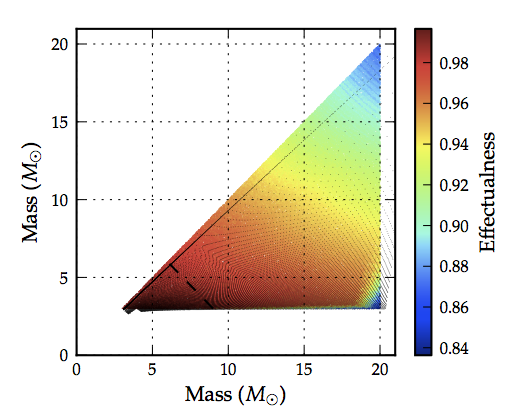
\includegraphics[scale=0.04, clip=false, totalheight=0.3\textheight, width=\columnwidth]{T4EOBeffectualness.pdf}
%\caption{\label{fig:match_t4eob_all}This figure shows the $\mathcal{FF}$ of a bank of Taylor T4 waveforms, with a minimal match of 0.97; at each point in the stellar-mass binary-black-hole region of the component-mass space. The color at each point is the maximum of overlap values between the full IMR EOB waveform for that point and the entire bank of Taylor T4 waveforms.}
%\end{figure}
%\begin{figure}
%\centering
%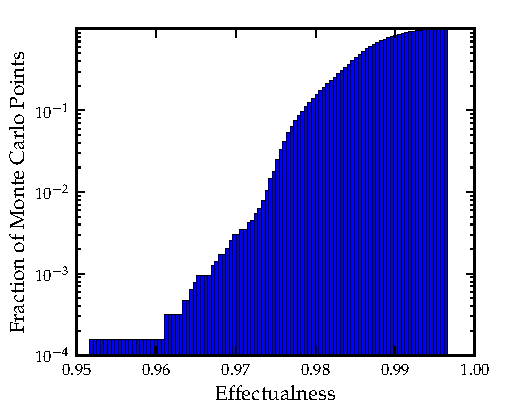
\includegraphics[scale=0.04, clip=false, totalheight=0.3\textheight, width=\columnwidth]{T4EOBhist.pdf}
%\caption{\label{fig:cumhist_t4eob_cut10}This figure shows a cumulative histogram of the fraction of the component-mass region, where the bank of Taylor T4 waveforms has $\mathcal{FF}$ less than the respective values on the x-axis. For example, over $0.04\%$ of the component-mass region, the T4 bank has $\mathcal{FF}$ below $0.965$. The component-mass region shown here has systems with individual component-masses in $(3-20)M_{\odot}$ and total mass below or equal to $12M_{\odot}$.}
%\end{figure}
%\begin{figure*}[]
%\centerline{
%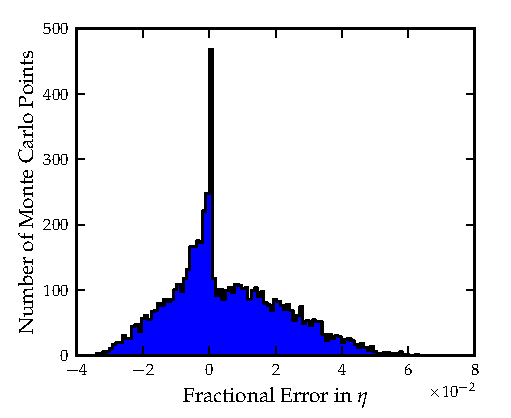
\includegraphics[scale=0.04, clip=false,keepaspectratio=true, width=\columnwidth]{hist_eta_err12paramT4EOB.pdf}\label{fig:errparams_t4eob_eta}              
%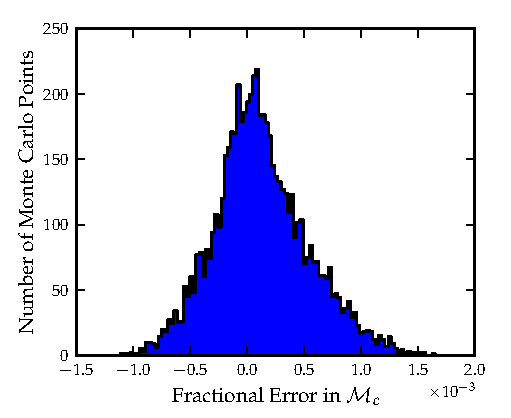
\includegraphics[scale=0.04, clip=false, keepaspectratio=true, width=\columnwidth]{hist_mchirp_err12paramT4EOB.pdf}\label{fig:errparams_t4eob_mchirp}
%}
%\caption{This figure shows the histogram of fractional difference between the physical parameters recovered by searching for the gravitational-wave signal using Taylor T4 bank of waveforms, and the actual physical parameters of the system used to generate the gravitational-wave signal. The left plot shows the fractional difference in the symmetric mass ratio $\eta$ and the right plot shows the fractional difference in the chirp mass $\mathcal{M}_c$. The designated component-mass-space region is the region with total mass below $12M_{\odot}$ and individual component-masses in $(3-20)M_{\odot}$.}
%\label{fig:errparams_t4eob}
%\end{figure*}
In this section we investigate the effectualness of the 2PN hexagonal template bank placement metric described in Ref.~\citep{BabaketalBankPlacement} when used to place EOBNRv2 waveform templates to cover the space of stellar-mass BBHs, having component masses between $3$ and $25\, M_{\odot}$. We also explore the efficiency of using the computationally cheaper Taylor F2 waveforms to search for a population of stellar-mass BBH signals modeled with the full EOBNRv2HM waveforms. We chose this approximant as the best available BBH model to provide a conservative bound on the use of Taylor F2-based searches. To assess the effectualness of the template banks, we compute the fitting factors \citep{FittingFactorApostolatos} for a population of random signals, with component masses drawn uniformly from $3$--$25\, M_\odot$. We define the fitting factor in the usual way, as follows. The frequency weighted overlap between two waveforms $h_1$ and $h_2$ is given by
\begin{equation}\label{eq:overlap}
(h_1|h_2) \equiv 2\int^{\infty}_0\dfrac{\tilde{h}_1^*(f)\tilde{h}_2(f) + \tilde{h}_1(f)\tilde{h}_2^*(f)}{S_n(f)}\D f,
\end{equation}
where $S_n(f)$ is the one-sided power spectral density (PSD) of the detector noise, and
\begin{equation}
\tilde{h}(f) = \int^{\infty}_{-\infty}e^{-2\pi\ii ft}h(t)\D t,
\end{equation}
is the Fourier transform of the waveform $h(t)$. We use the Zero-Detuned-High-Power PSD estimate for aLIGO \citep{aLIGONoiseCurve}. The normalized overlap between the two waveforms is given by
\begin{equation}
(\hat{h}_1|\hat{h}_2) = \dfrac{(h_1|h_2)}{\sqrt{(h_1|h_1)(h_2|h_2)}}.
\end{equation}
In addition to the two mass-parameters of the binary, this normalized overlap is also sensitive to the relative phase of coalescence $\phi_c$ and to the difference in the time of coalescence $t_c$ between the two waveforms $h_1$ and $h_2$. These two parameters ($\phi_c$ and $t_c$) can be analytically maximized over to get the maximized overlap $\Olap$ (for details, see Chap.[4] of Ref. \citep{Brown:2004vh}),
\begin{equation}\label{eq:maxnormolap}
\Olap(h_1,h_2) = \underset{\phi_c,t_c}{\mathrm{max}}\,\l(\hat{h}_1|\hat{h}_2(\phi_c,t_c)\r),
\end{equation}
which gives a measure of how ``close'' the two waveforms are in the waveform manifold. The mismatch $\mathcal{M}$ between the same two waveforms is written as,
\begin{equation}\label{eq:mismatch}
\mathcal{M}(h_1,h_2) = 1 - \Olap(h_1,h_2).
\end{equation}
If $h^e_a$ is the waveform emitted by a BBH system then the \textit{Fitting Factor} of a bank of template waveforms (modeled using approximant $\X$) for this waveform, is defined as the maximum value of maximized normalized overlaps between $h^e_a$ and all members $h^{\X}_b$ of the bank of template waveforms \citep{FittingFactorApostolatos}; i.e.
\begin{equation}\label{eq:defFF}
\mathcal{FF}(a,\X) = \underset{b\, \in\, \mathrm{bank}}{\textrm{max}}\,\Olap(h^e_a,h^{\X}_b).
\end{equation}
This quantity simultaneously quantifies the loss in recovered signal-to-noise ratio (SNR) due to the discreteness of the bank, and the inaccuracy of the template model. The similarly defined quantity $\MM$ (minimal match) quantifies the loss in SNR due to only the discreteness of the bank, as both the \textit{exact} and the template waveform is modeled with the same waveform model, i.e.
\begin{equation}
\MM = \underset{a}{\textrm{min}}\,\underset{b\, \in\, \mathrm{bank}}{\textrm{max}}\,\Olap(h^{\X}_a,h^{\X}_b),
\end{equation}
where $a$ is any point in the space covered by the bank, and $\X$ is the waveform approximant. For a detection search that aims at less than $10\%\, (15\%)$ loss in event detection rate due to the discreteness of the bank and the inaccuracy of the waveform model, we require a bank of template waveforms that has $\mathcal{FF}$ above $0.965\, (0.947)$ \citep{WaveformAccuracy2008,WaveformAccuracy2010,CompTemplates2009}.

\subsection{Template Placement of EOBNRv2}\label{sec:level2:EOBNRv2templateplacement}
\begin{figure}
	\begin{center}
		\scalebox{1}{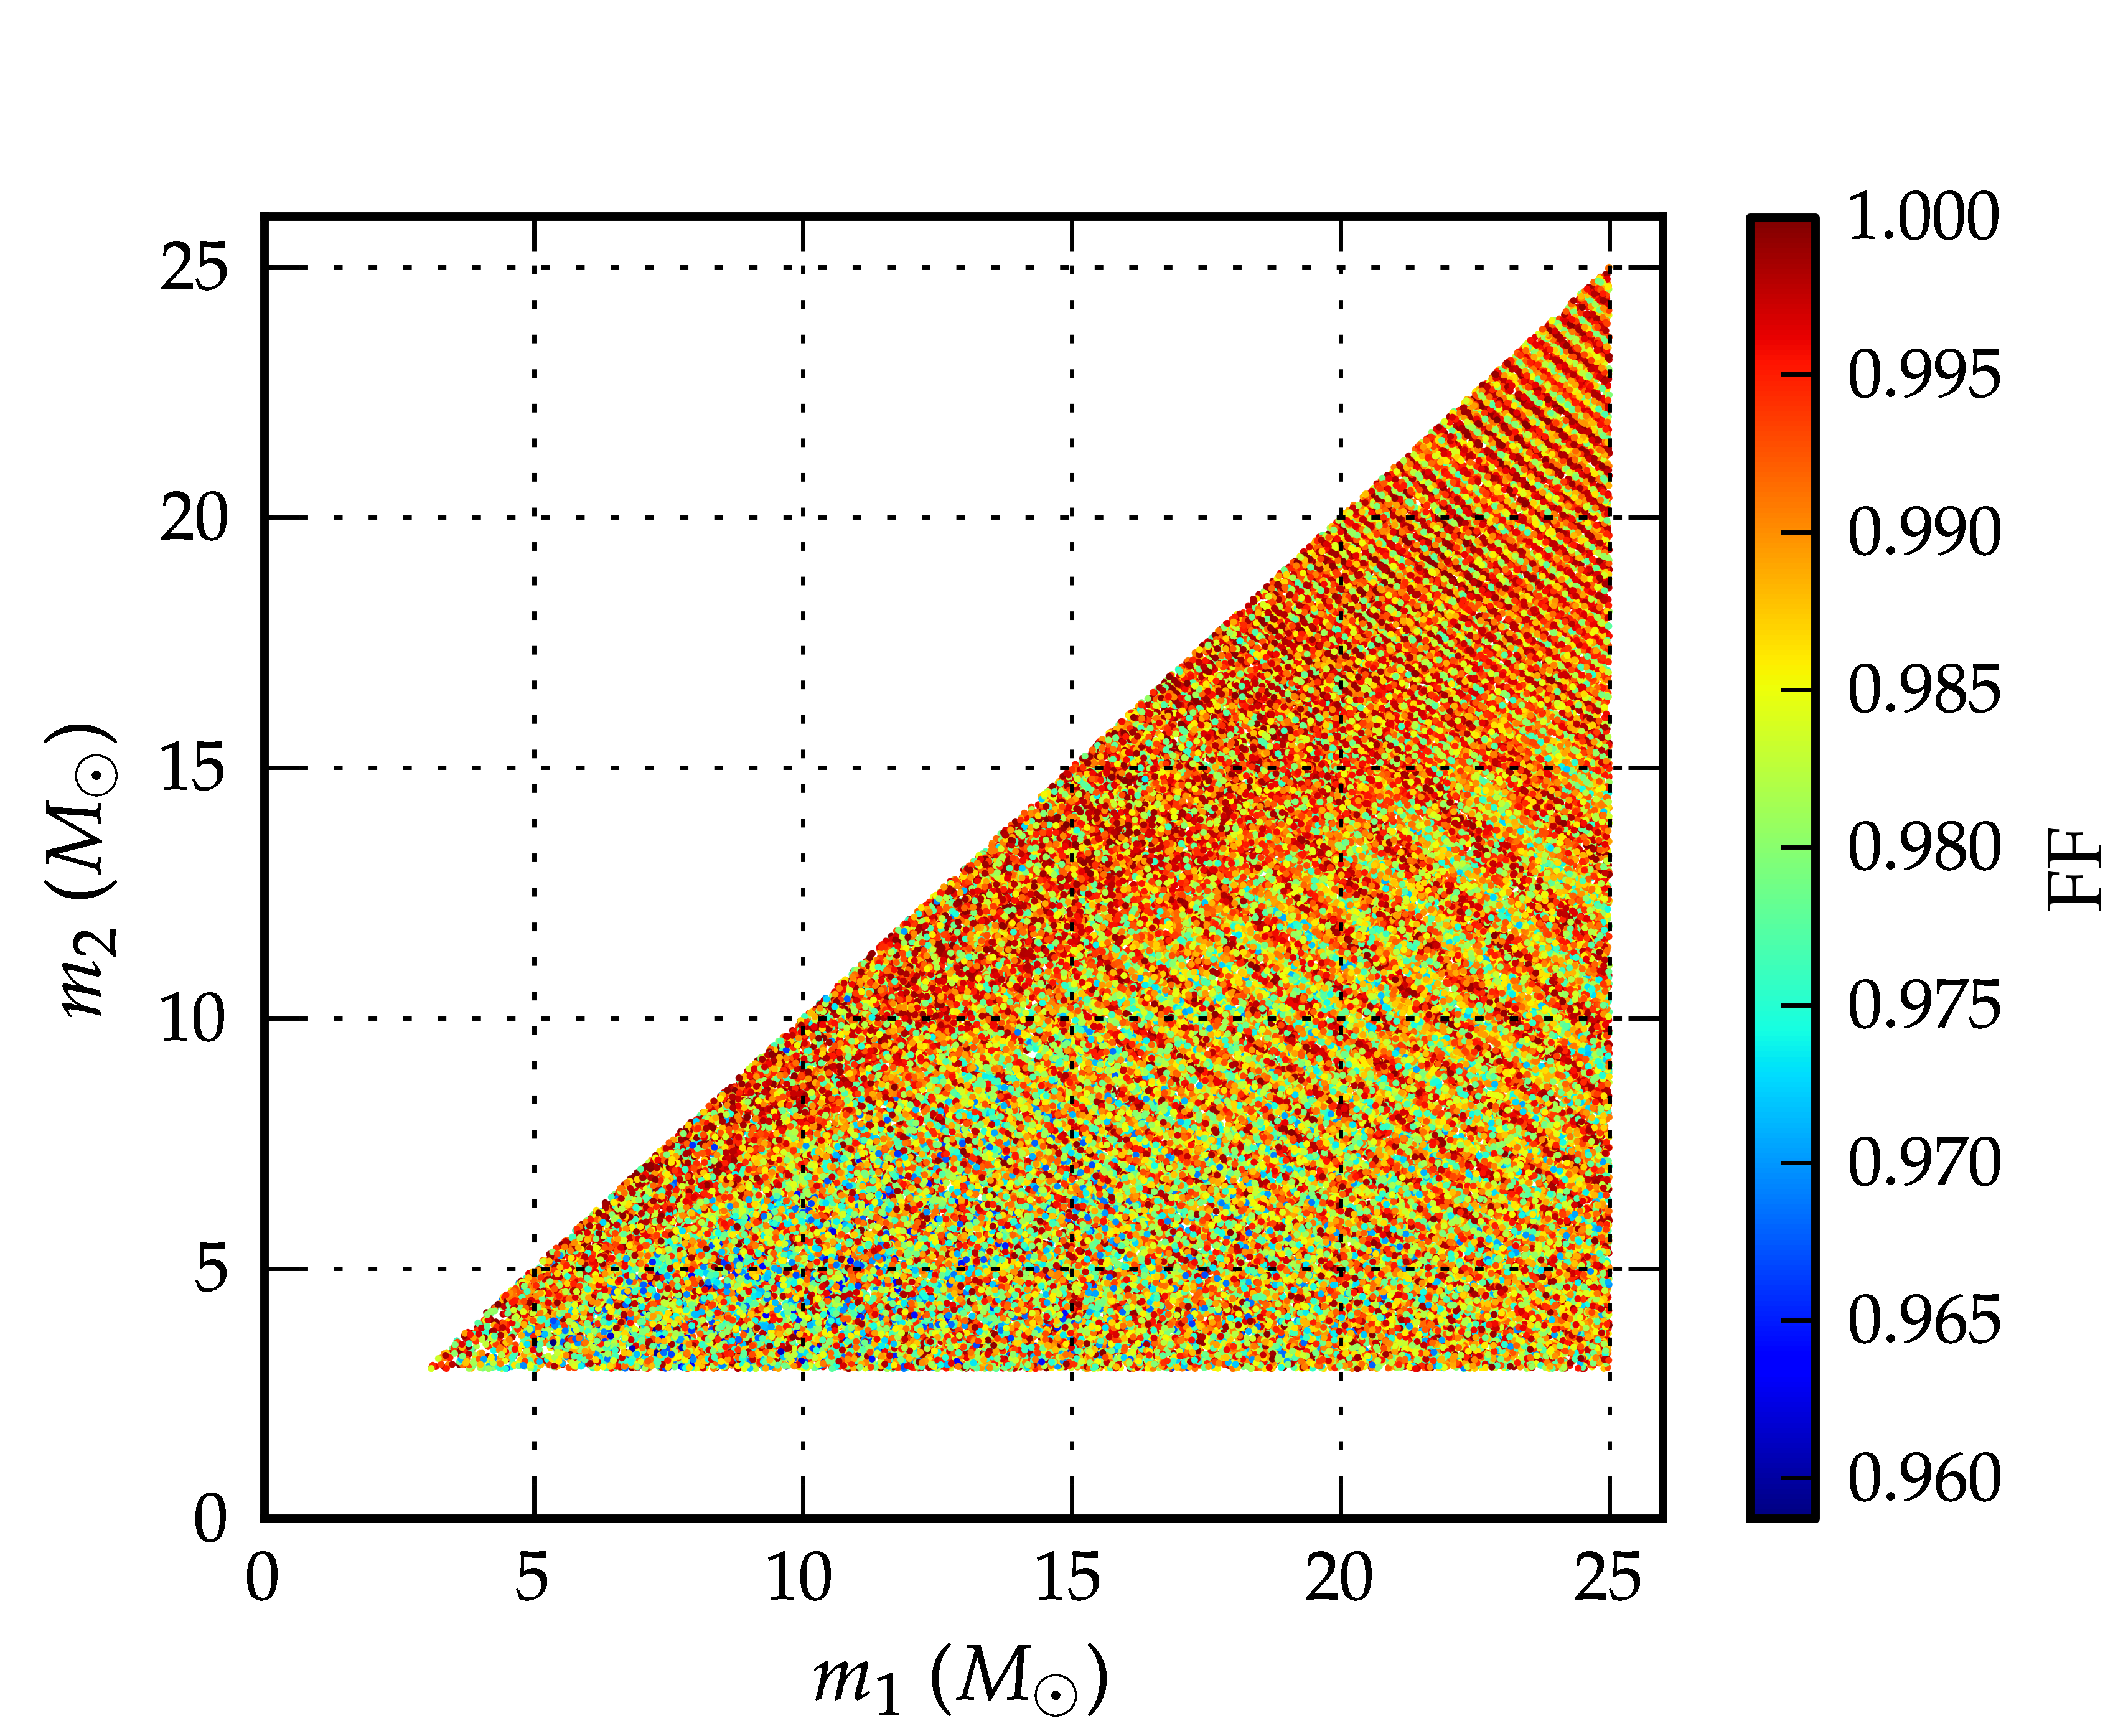
\includegraphics[width=\columnwidth]{EOB22vsEOB22FULL.png}} % XXX large figure
	\end{center}
\caption{This figure shows the effectualness of a bank of EOBNRv2 templates, placed using the 2PN accurate hexagonal template placement of Ref.~\citep{BabaketalBankPlacement} to search for a population of BBH signals simulated with EOBNRv2 waveforms. The masses of the BBH population are chosen from a uniform distribution of component masses between $3$ and $25\, M_{\odot}$. For each injection, we plot the component masses of the injection and the fitting factor $\l(\FF\r)$.}
\label{fig:match_eobeob_all}
\end{figure}

\begin{figure}
	\begin{center}
		\scalebox{1}{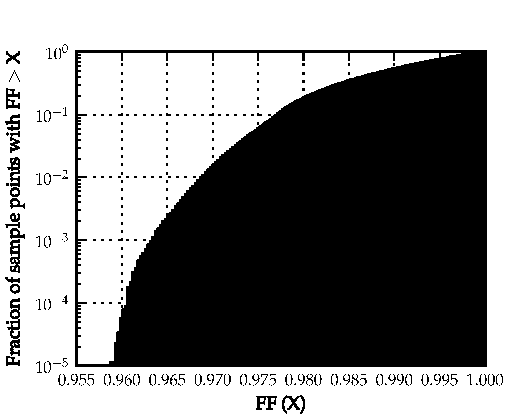
\includegraphics[clip=false, totalheight=0.3\textheight, width=\columnwidth]{EOB22vsEOB22FULLcumhist.pdf}}
	\end{center}
\caption{This figure shows a cumulative histogram of the fraction of the component-mass region (on the y-axis), where the bank of EOBNRv2 waveforms has $\mathcal{FF}^E$ less than the respective values on the x-axis. For example, over $\sim 1.5\%$ of the component-mass region, the EOBNRv2 bank has $\mathcal{FF}^E$ below the $0.97$. The component-mass region shown here has BBH systems with individual component-masses in $(3-25)M_{\odot}$.}
\label{fig:cumhist_eobeob_all}
\end{figure} 
The 2PN Owen-Sathya metric \citep{SathyaMetric2PN} gives the mismatch $\mathcal{M}$ between two waveforms, if the source BBH of one of the waveforms has mass parameters \textit{slightly} different from the mass parameters of the source BBH of the other waveform. This is defined in Eqn. [2.8] of Ref.~\citep{SathyaMetric2PN}. Using this metric, one can place points in the component-mass space in a way that they are uniformly gridded in terms of the $\mathcal{M}$ between the waveforms for any neighboring points. This lets us create a discrete bank of templates that is uniformly gridded in $\mathcal{M}$ \citep{BabaketalBankPlacement}. Such banks, with 3.5PN Taylor F2 waveforms, were used in detection searches for initial LIGO data \citep{Colaboration:2011nz,Abadie:2010yb,Abbott:2009qj,Abbott:2009tt,Messaritaki:2005wv}. But the metric itself was derived using frequency domain Taylor F2 waveforms, accurate to 2PN order in GW phase. Thus, \textit{a priori} one does not know if this metric will prove to be a good 
measure to use to generate template banks of EOBNRv2 waveforms.

We do a Monte-Carlo simulation over the entire stellar-mass BBH mass region to find regions where the hexagonal bank placement algorithm leads to under-coverage. The exact waveform $h^e$ is approximated by EOBNRv2 waveforms. The simulation was done by sampling 90,000 points over the designated region of the component-mass space, uniformly distributed in individual component-mass. For each of these points, we generate the EOBNRv2 waveform for the system with component masses given by the coordinates of the point, starting from the time when the gravitational-wave frequency from the system crosses 15Hz, and ending when the quasi-normal ringing of the final black-hole (formed by the coalescence of the binary) ends. Next, we generate a bank of EOBNRv2 waveforms, gridded using the 2PN Owen-Sathya bank placement metric, covering the same mass region. This bank is generated with the requirement that the waveform generated for \textit{any} point $j$ in that mass-region will have a maximized normalized overlap $\geq 
0.97$ with \textit{at least} one point in the bank; i.e., $\Olap(h^{\X}_j,h^{\X}_k)\geq 0.97$ for at least one point $k$ in the bank (the superscript $\X$ denotes the waveform model used to generate $h$, which here is EOBNRv2). This is the same as requiring that $\MM=0.97$. We record the $\mathcal{FF}$ of the template bank at all the Monte-Carlo points. For each point $a$, we calculate the maximum of maximized overlaps between the EOBNRv2 waveform at that point and the entire bank of EOBNRv2 waveforms, $\mathcal{FF}^E$,
\begin{equation}
\mathcal{FF}^E(a) = \underset{b\,\in\,\mathrm{bank}}{\mathrm{max}}\,\Olap(h^{\X}_a,h^{\X}_b),
\end{equation}
where $b$ is any element of the discrete set of points in the component-mass space that constitutes the template bank. Since we use EOBNRv2 to model the true GW signals and also to model the templates, any departure of the $\FF^E$ from unity would solely be an artifact of the coarseness of the template bank grid. For a bank of template waveforms that was constructed with an intended $\MM$ of $0.97$, we see in Fig.~\ref{fig:match_eobeob_all} and Fig.~\ref{fig:cumhist_eobeob_all} that the $\mathcal{FF}^E$ of the bank remains above $0.97$ over $\sim 98.5\%$ of the designated mass space. For fewer than $\sim 1.5\%$ of the sampled BBH systems, does the $\mathcal{FF}^E$ of the bank fall below 0.97. The least value of $\mathcal{FF}^E$, over the 90,000 sampled points, was found to be $\sim 0.96$. The stripe features observed in Fig.~\ref{fig:match_eobeob_all} are features of the hexagonal bank placement algorithm and is related to the ellipses in Fig.[4] of Ref.~\citep{BabaketalBankPlacement}. We observe a 
systematic decrease in the $\FF$ between the mismatch ellipses given by the bank placement metric, hinting at a systematic overestimation of the overlap between the neighboring templates by the Owen-Sathya metric (leading to systemic under-coverage between them).

From these results, its evident that the 2PN bank placement metric does well in covering the BBH mass space adequately with EOBNRv2 waveform templates, that are accurate to pseudo-5PN. This result demonstrates that detection searches in aLIGO, which would use EOB waveform templates, can employ the 2PN Owen-Sathya bank placement metric to place template banks without a significant drop in recovered SNR due to the coarseness of the bank grid.

\subsection{Taylor F2 Bank}\label{sec:level2:EffectualnessTaylorF2}
%\begin{figure}
%\centering
%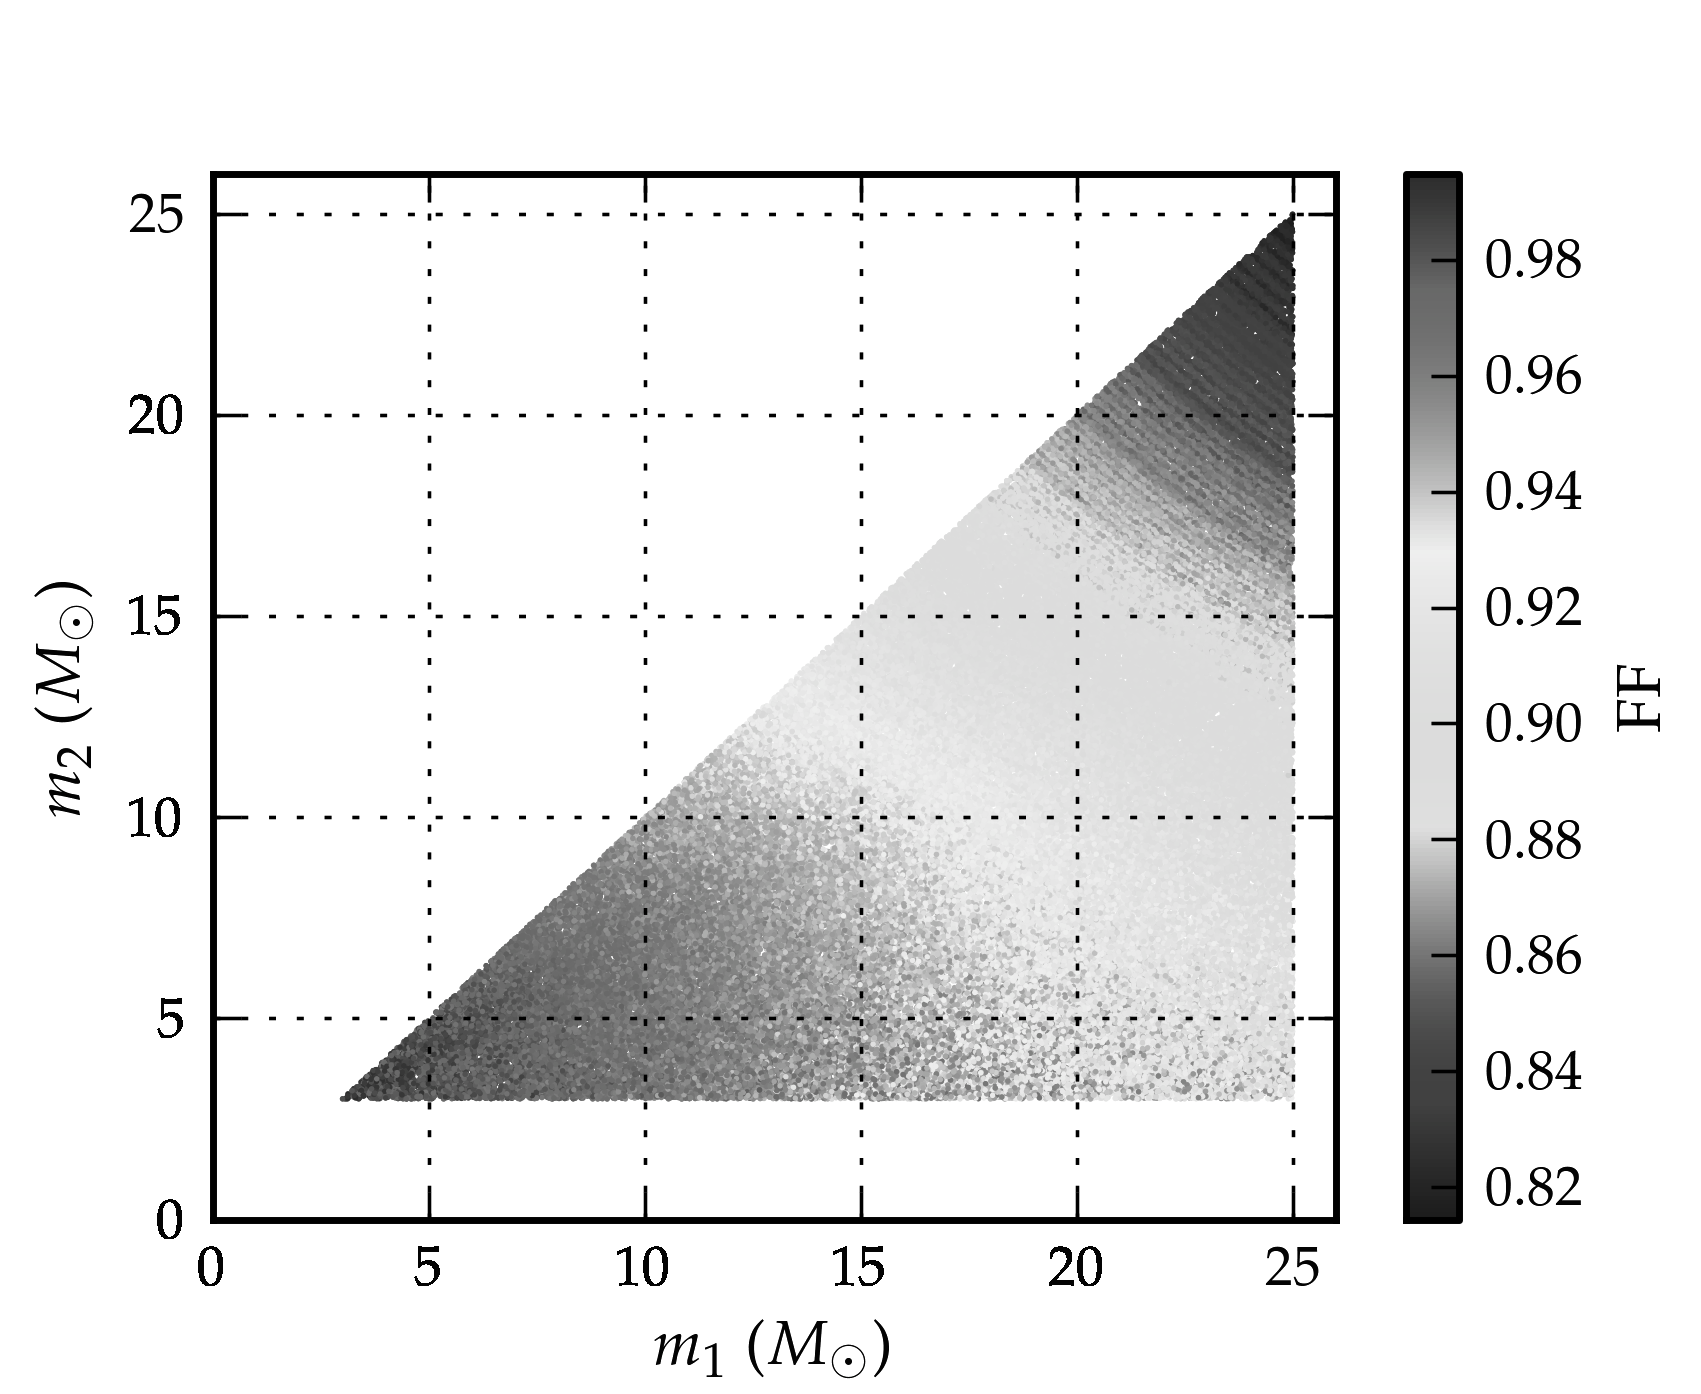
\includegraphics[scale=0.04, clip=false, totalheight=0.3\textheight, width=\columnwidth]{EOBHMvsF2FULLNolines.png} % XXX large figure
%\caption{\label{fig:match_f2eob_all}This figure shows the fitting factor $\mathcal{FF}$ of a bank of Taylor F2 waveforms, constructed with $\MM = 0.97$ at each point in the stellar-mass BBH region of the component-mass space. The color at each point is the maximum of all overlap values between the complete inspiral-merger-ringdown EOB waveform for that point and the entire bank of Taylor F2 waveforms (i.e. $\FF$).}
%%The green (blue) line in the figure denotes the region with $M<8.8M_{\odot}\, (14M_{\odot})$, in which the $\FF$ of the Taylor F2 bank is above the threshold of $0.965\, (0.947)$.
%\end{figure}

%\begin{figure*}
%\centerline{
%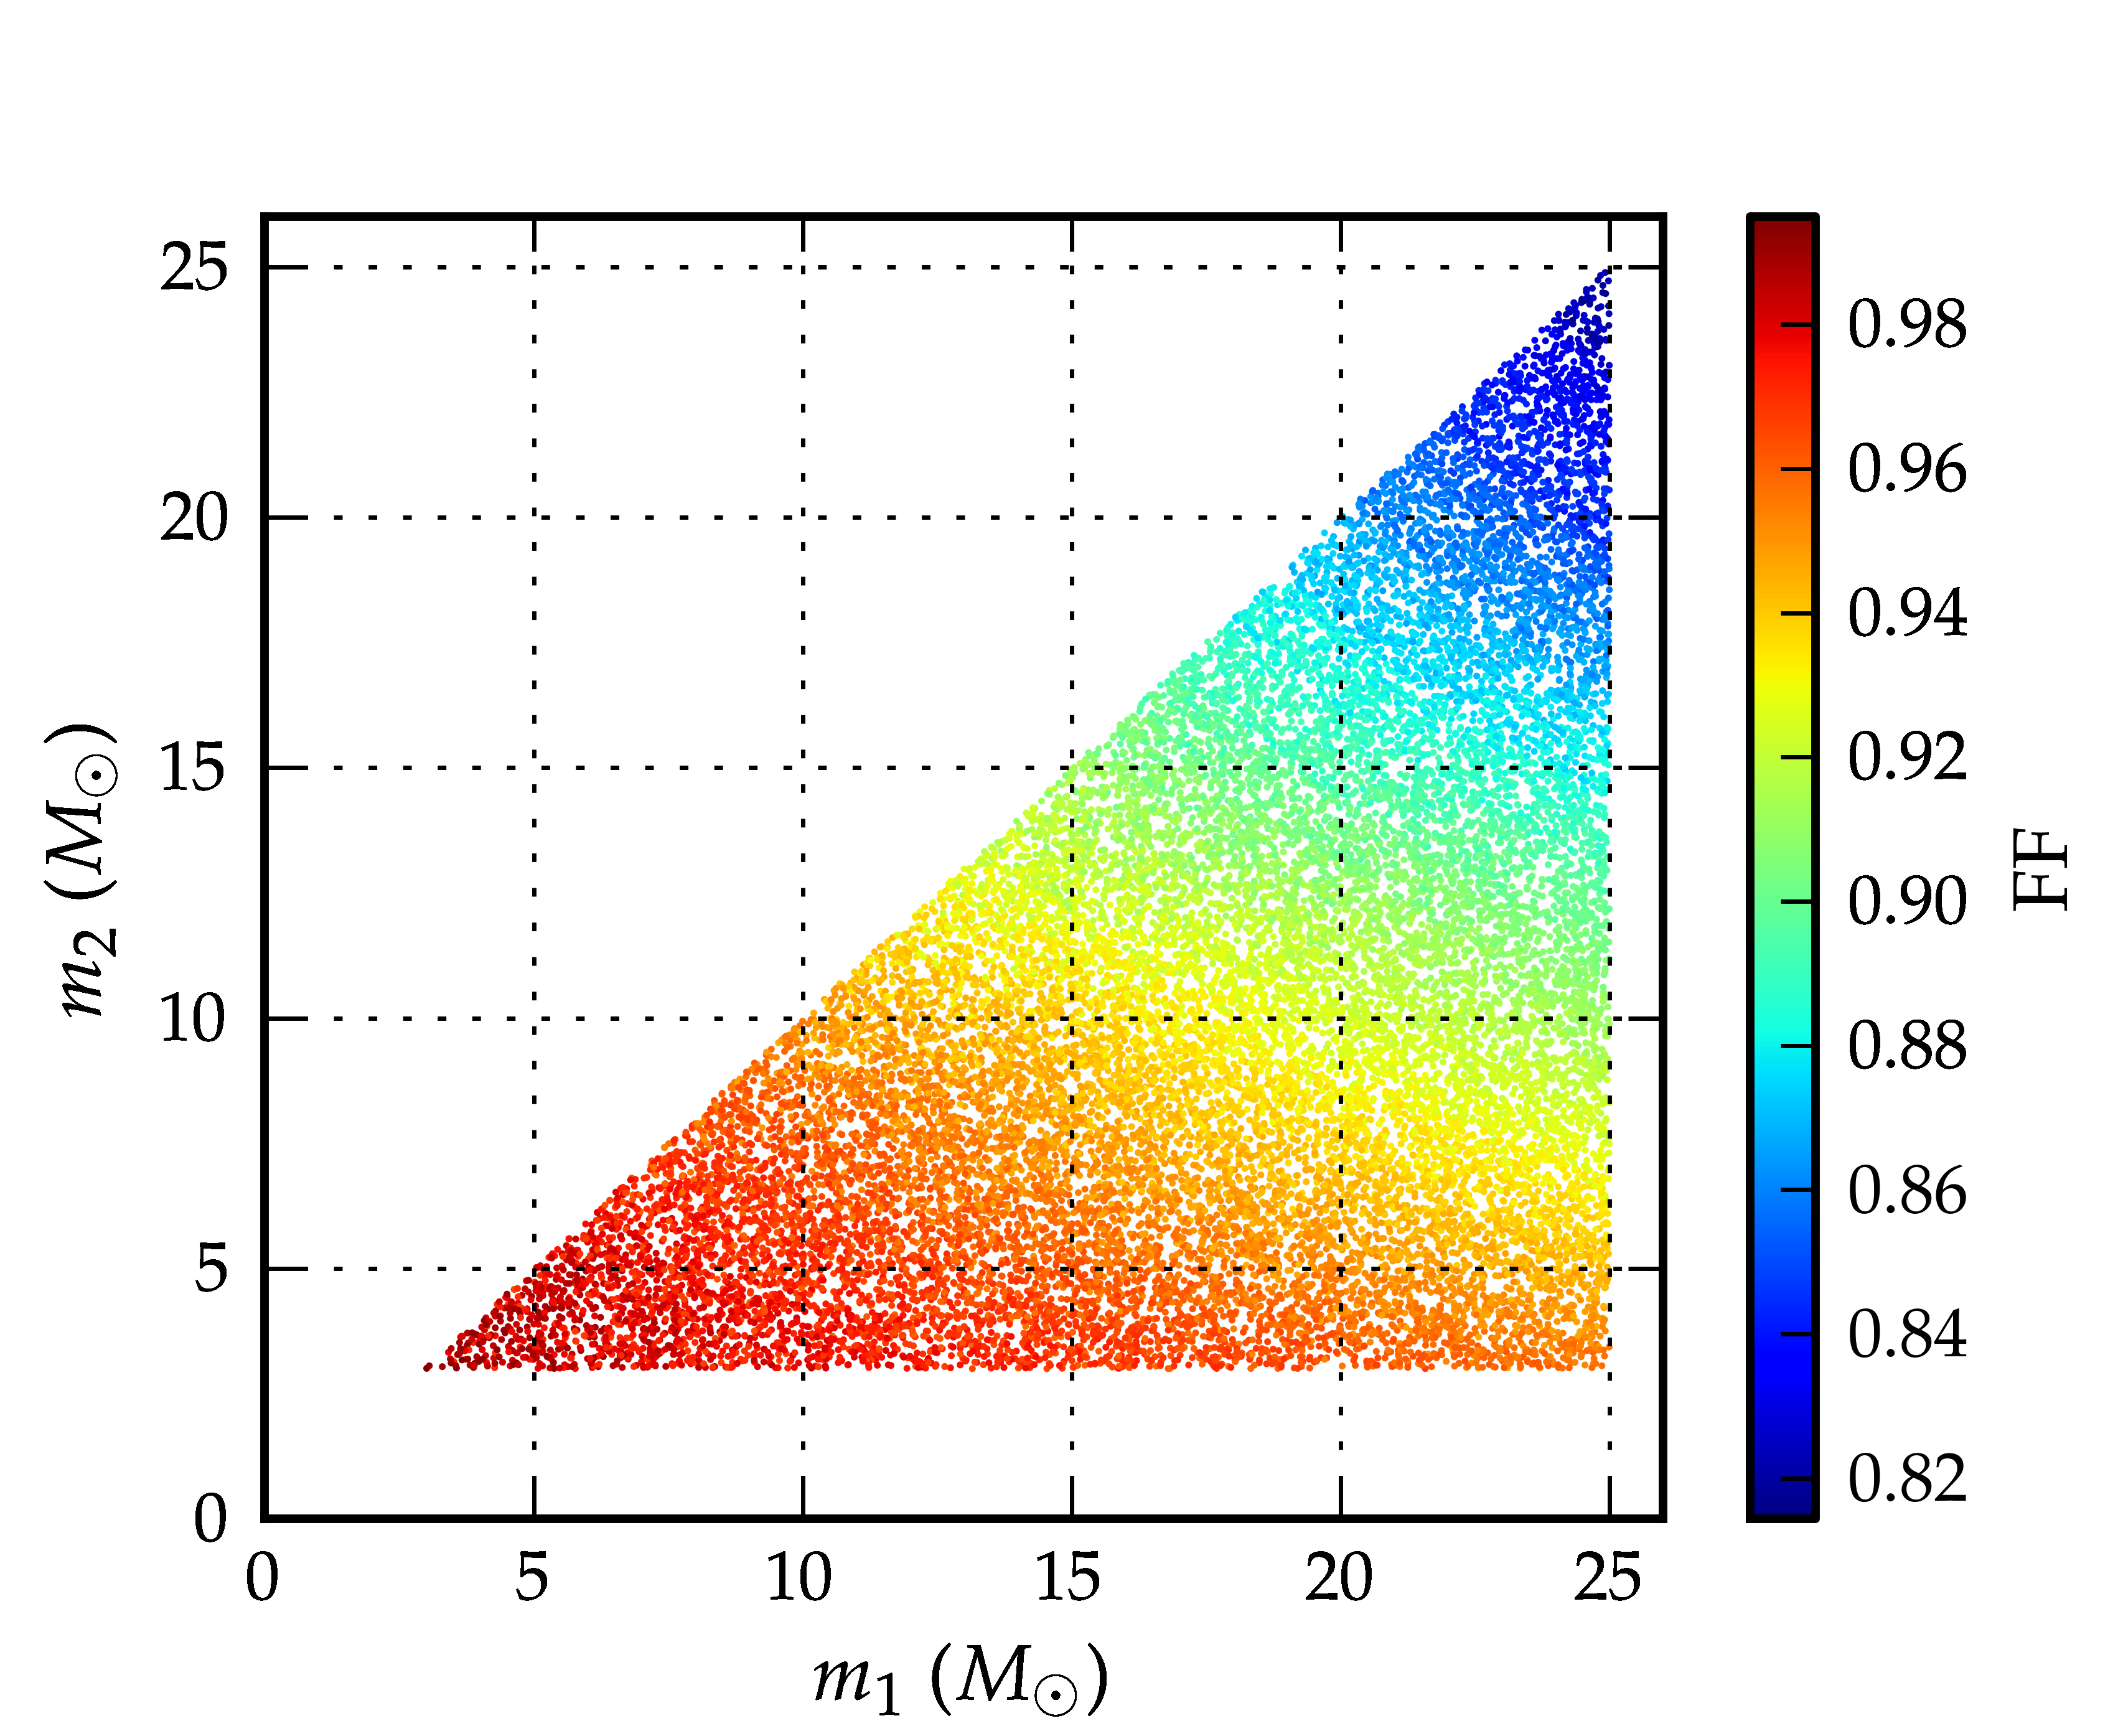
\includegraphics[scale=0.04, clip=false,keepaspectratio=true, width=\columnwidth]{EOB22vsF2FULLNolines.png}
%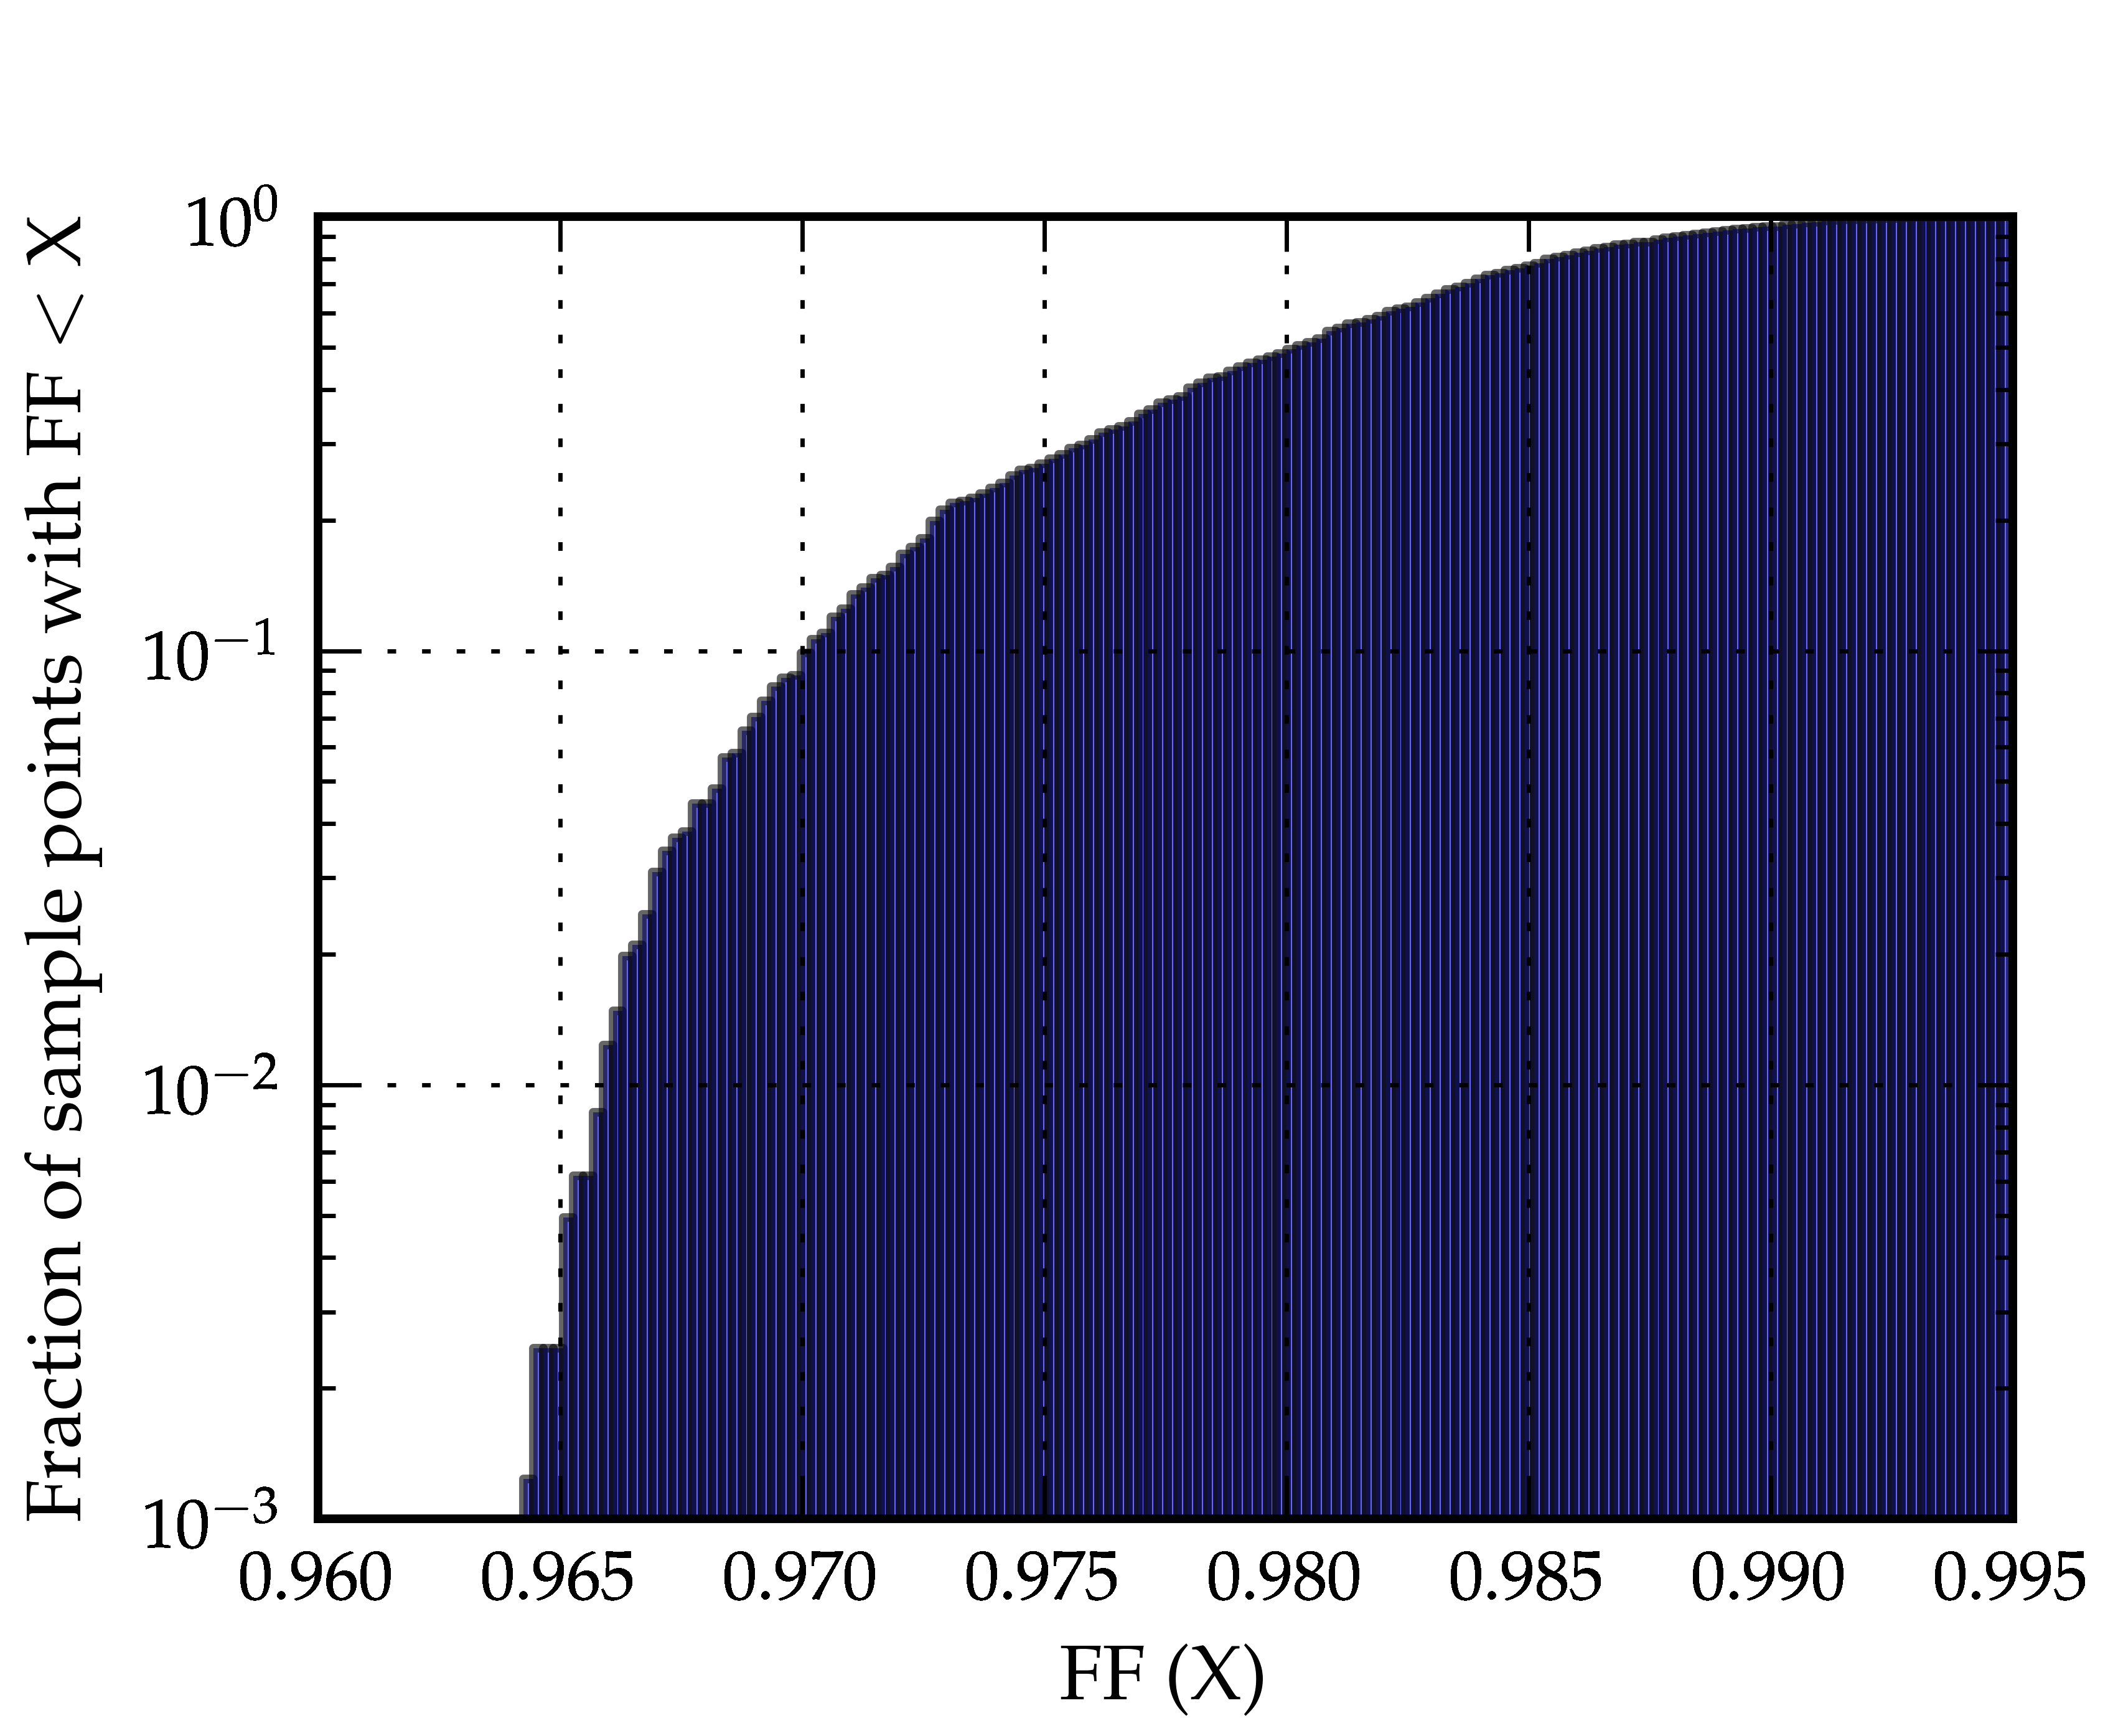
\includegraphics[scale=0.04, clip=false, keepaspectratio=true, width=\columnwidth]{EOB22vsF2cutcumhist12.png}
%}
%\caption{\label{fig:match_cumhist_f2eob22_cut12}The figure on the left is identical to Fig.\ref{fig:match_eobeob_all}, with the difference that the fitting factors of the bank of Taylor F2 waveforms shown here are calculated against inspiral-merger-ringdown EOB waveforms which do not include sub-leading waveform multipoles. The figure on the right shows the cumulative histogram of the the fitting factors of the bank of Taylor F2 waveforms with the leading order EOB waveforms, over the component mass region with total masses below $12M_{\odot}$.}
%\end{figure*}

\begin{figure*}
\centerline{
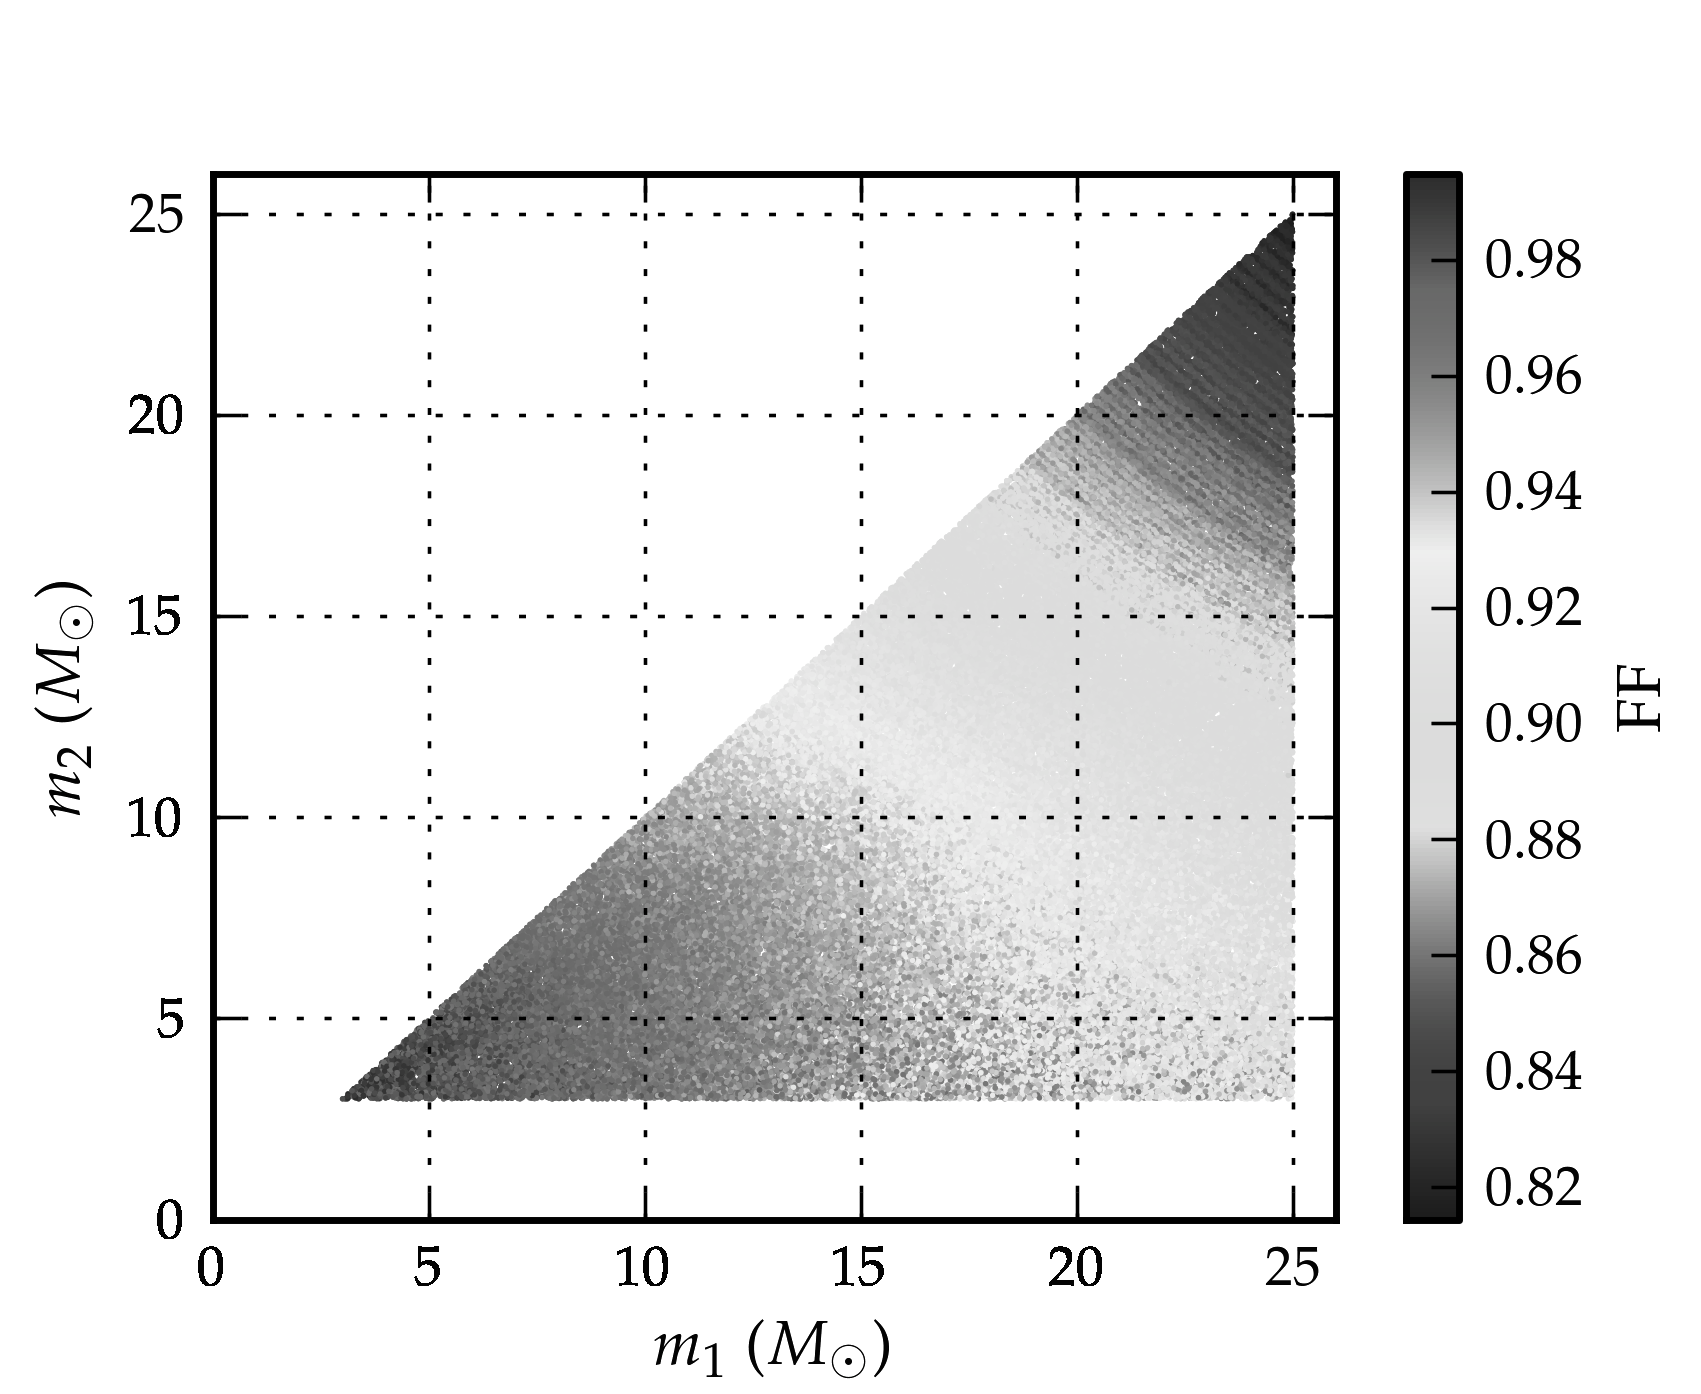
\includegraphics[scale=0.04, clip=false, keepaspectratio=true, width=\columnwidth]{EOBHMvsF2FULLNolines.png} % XXX large figure
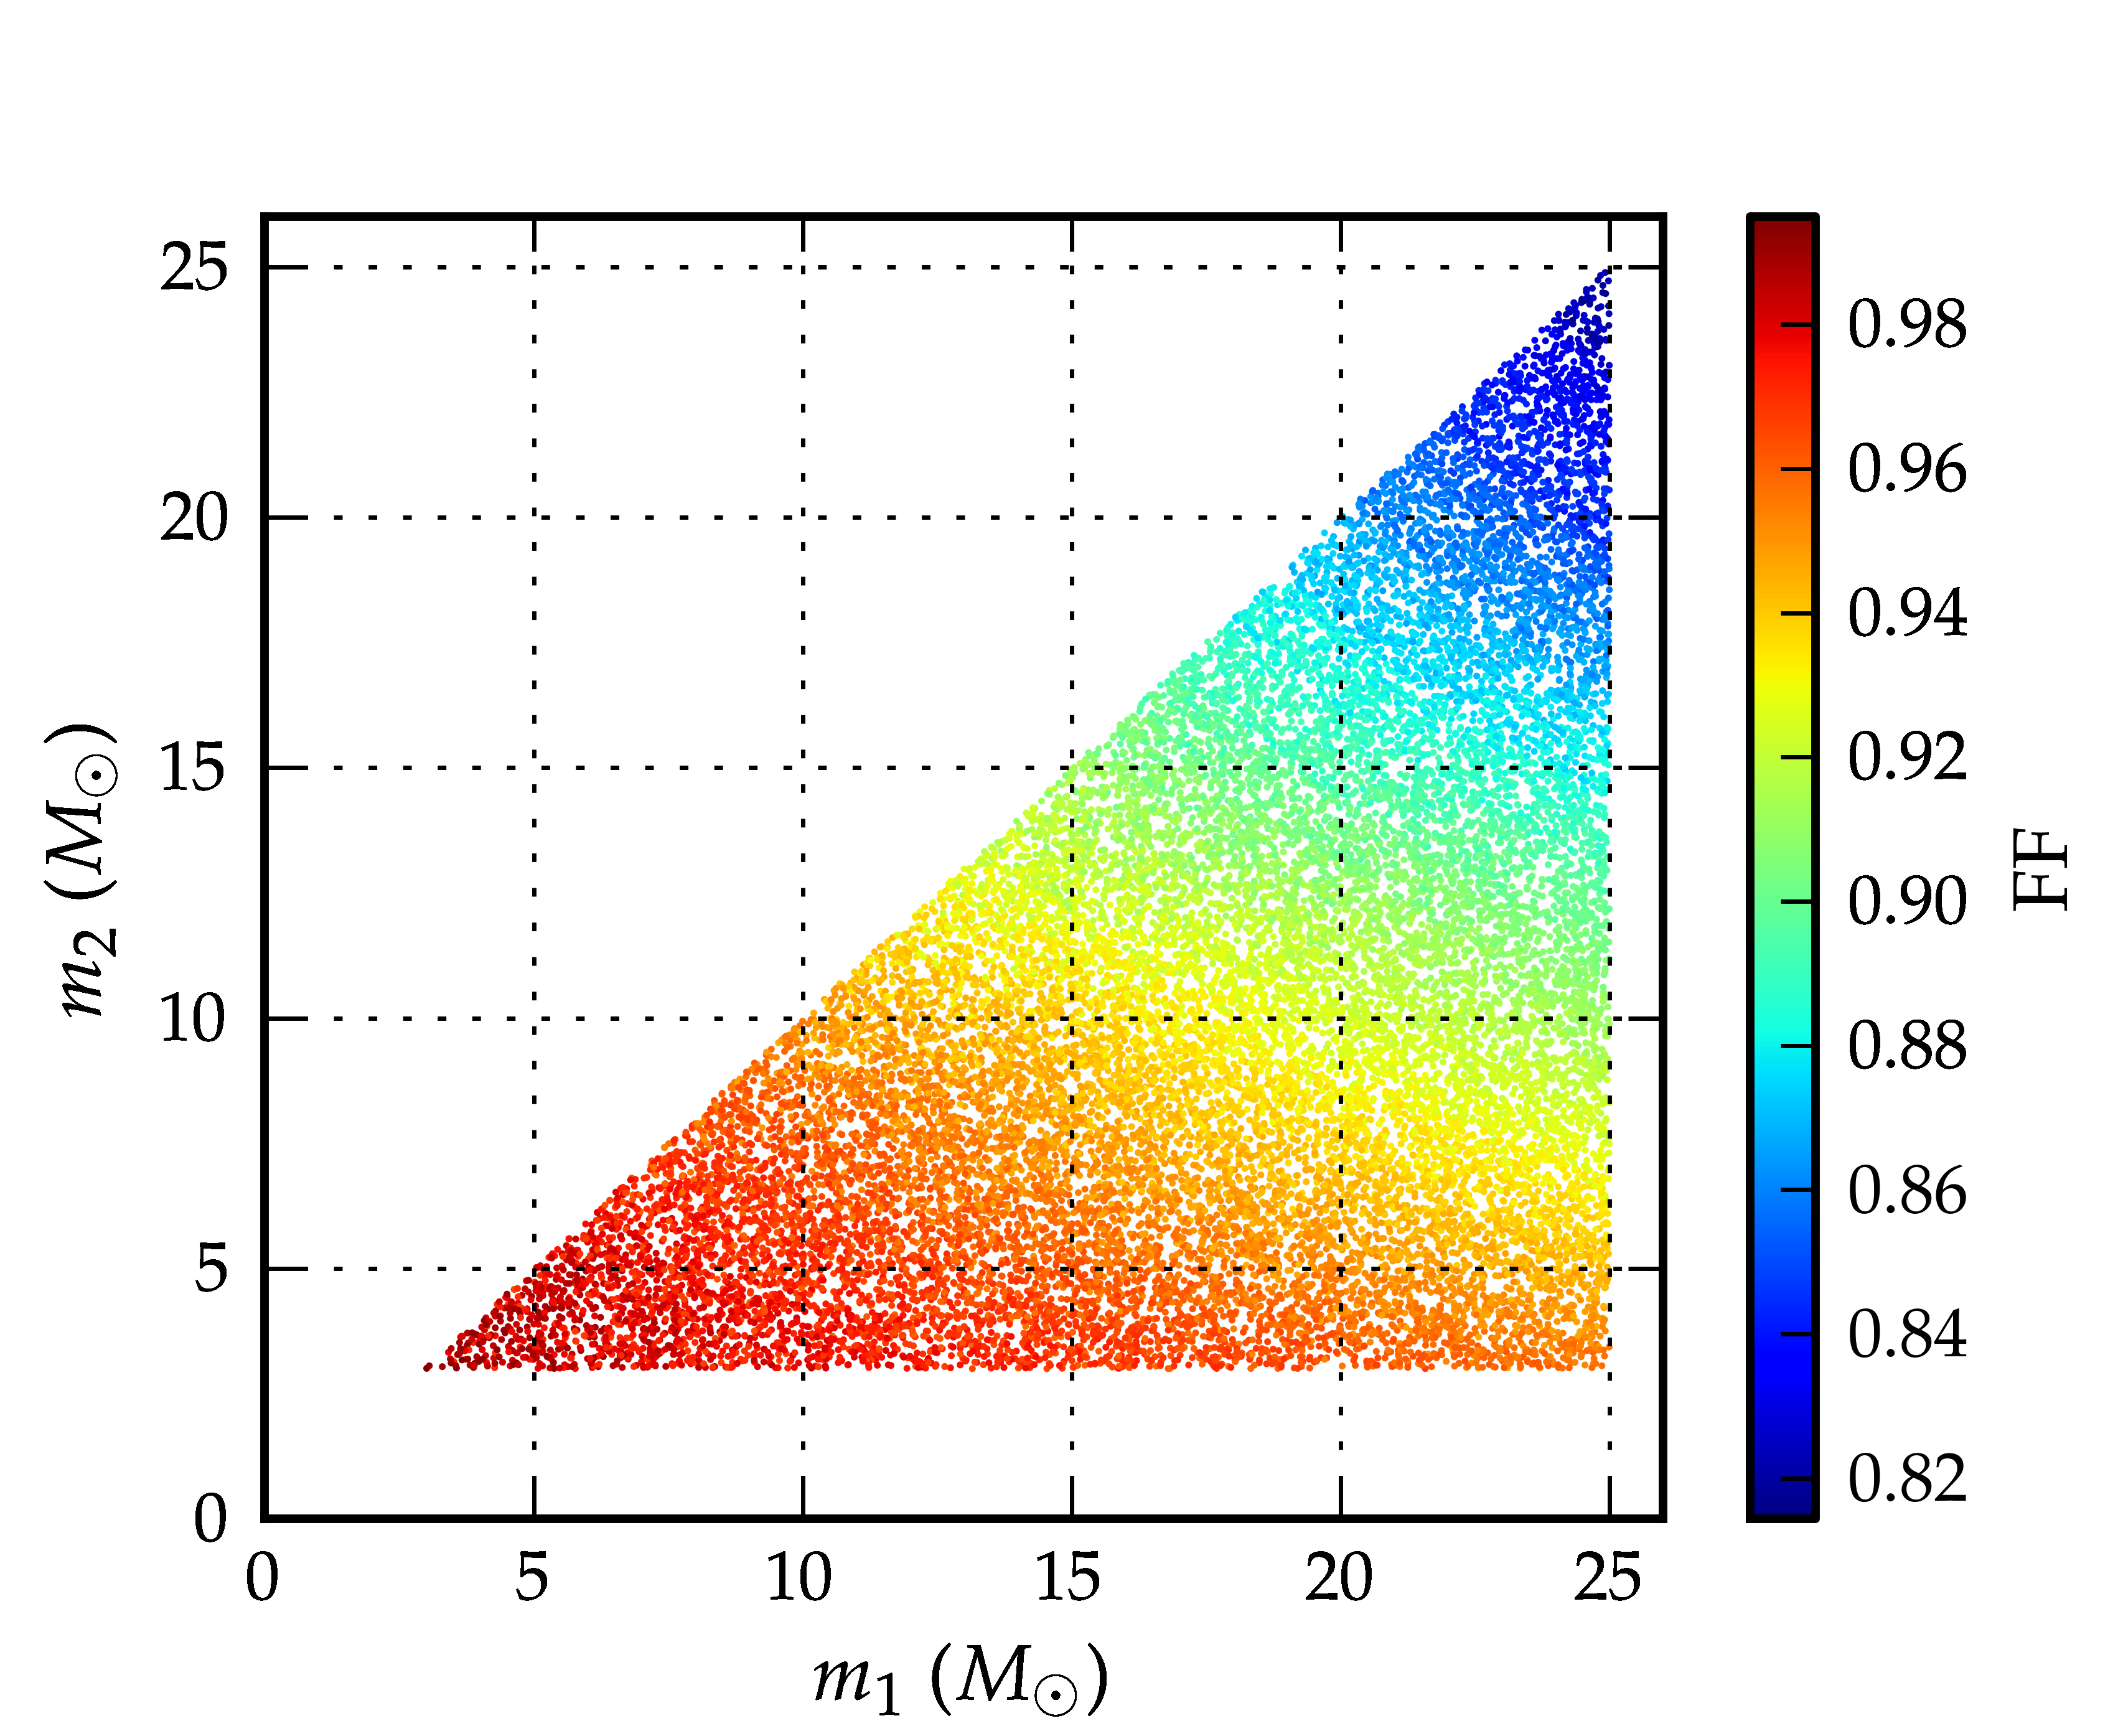
\includegraphics[scale=0.04, clip=false, keepaspectratio=true, width=\columnwidth]{EOB22vsF2FULLNolines.png} % XXX large figure
}
\caption{\label{fig:match_f2eob_f2eob22_all}These figures show the fitting factor $\mathcal{FF}$ of a bank of Taylor F2 waveforms, constructed with $\MM = 0.97$. Each point in the left (right) figure, shows the $\FF$ against inspiral-merger-ringdown EOB waveforms with (without) sub-leading waveform multipoles, generated for the mass values (coordinates) for that point.}
\end{figure*}

\begin{figure*}
\centerline{
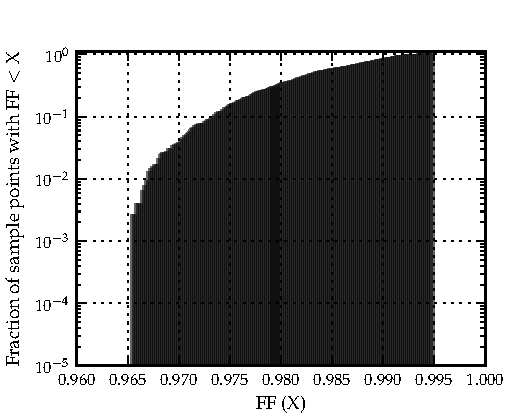
\includegraphics[scale=0.04, clip=false,keepaspectratio=true, width=\columnwidth]{EOBHMvsF2cutcumhist8-8.pdf}
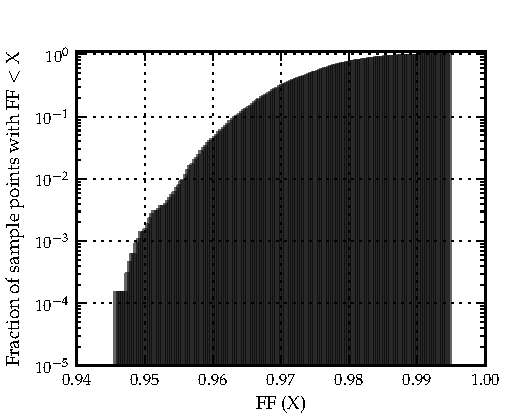
\includegraphics[scale=0.04, clip=false, keepaspectratio=true, width=\columnwidth]{EOBHMvsF2cutcumhist14.pdf}
}
\caption{\label{fig:cumhist_f2eob_cut14}These figure show cumulative histograms of the fraction of the component-mass region where the bank of Taylor F2 waveforms has fitting factors less than the respective values on the x-axis. The component-mass region shown here has systems with individual component-masses between $(3-25)M_{\odot}$, and total mass below or equal to $8.8M_{\odot}$ (left) and $14M_{\odot}$ (right). The plot shows that for more than $99.9\%$ of the points sampled in the entire designated part of the component-mass region, the Taylor F2 bank has $\mathcal{FF}$ above $0.965$ (left) and above $0.947$ (right).}
\end{figure*}

\begin{figure}
\centering
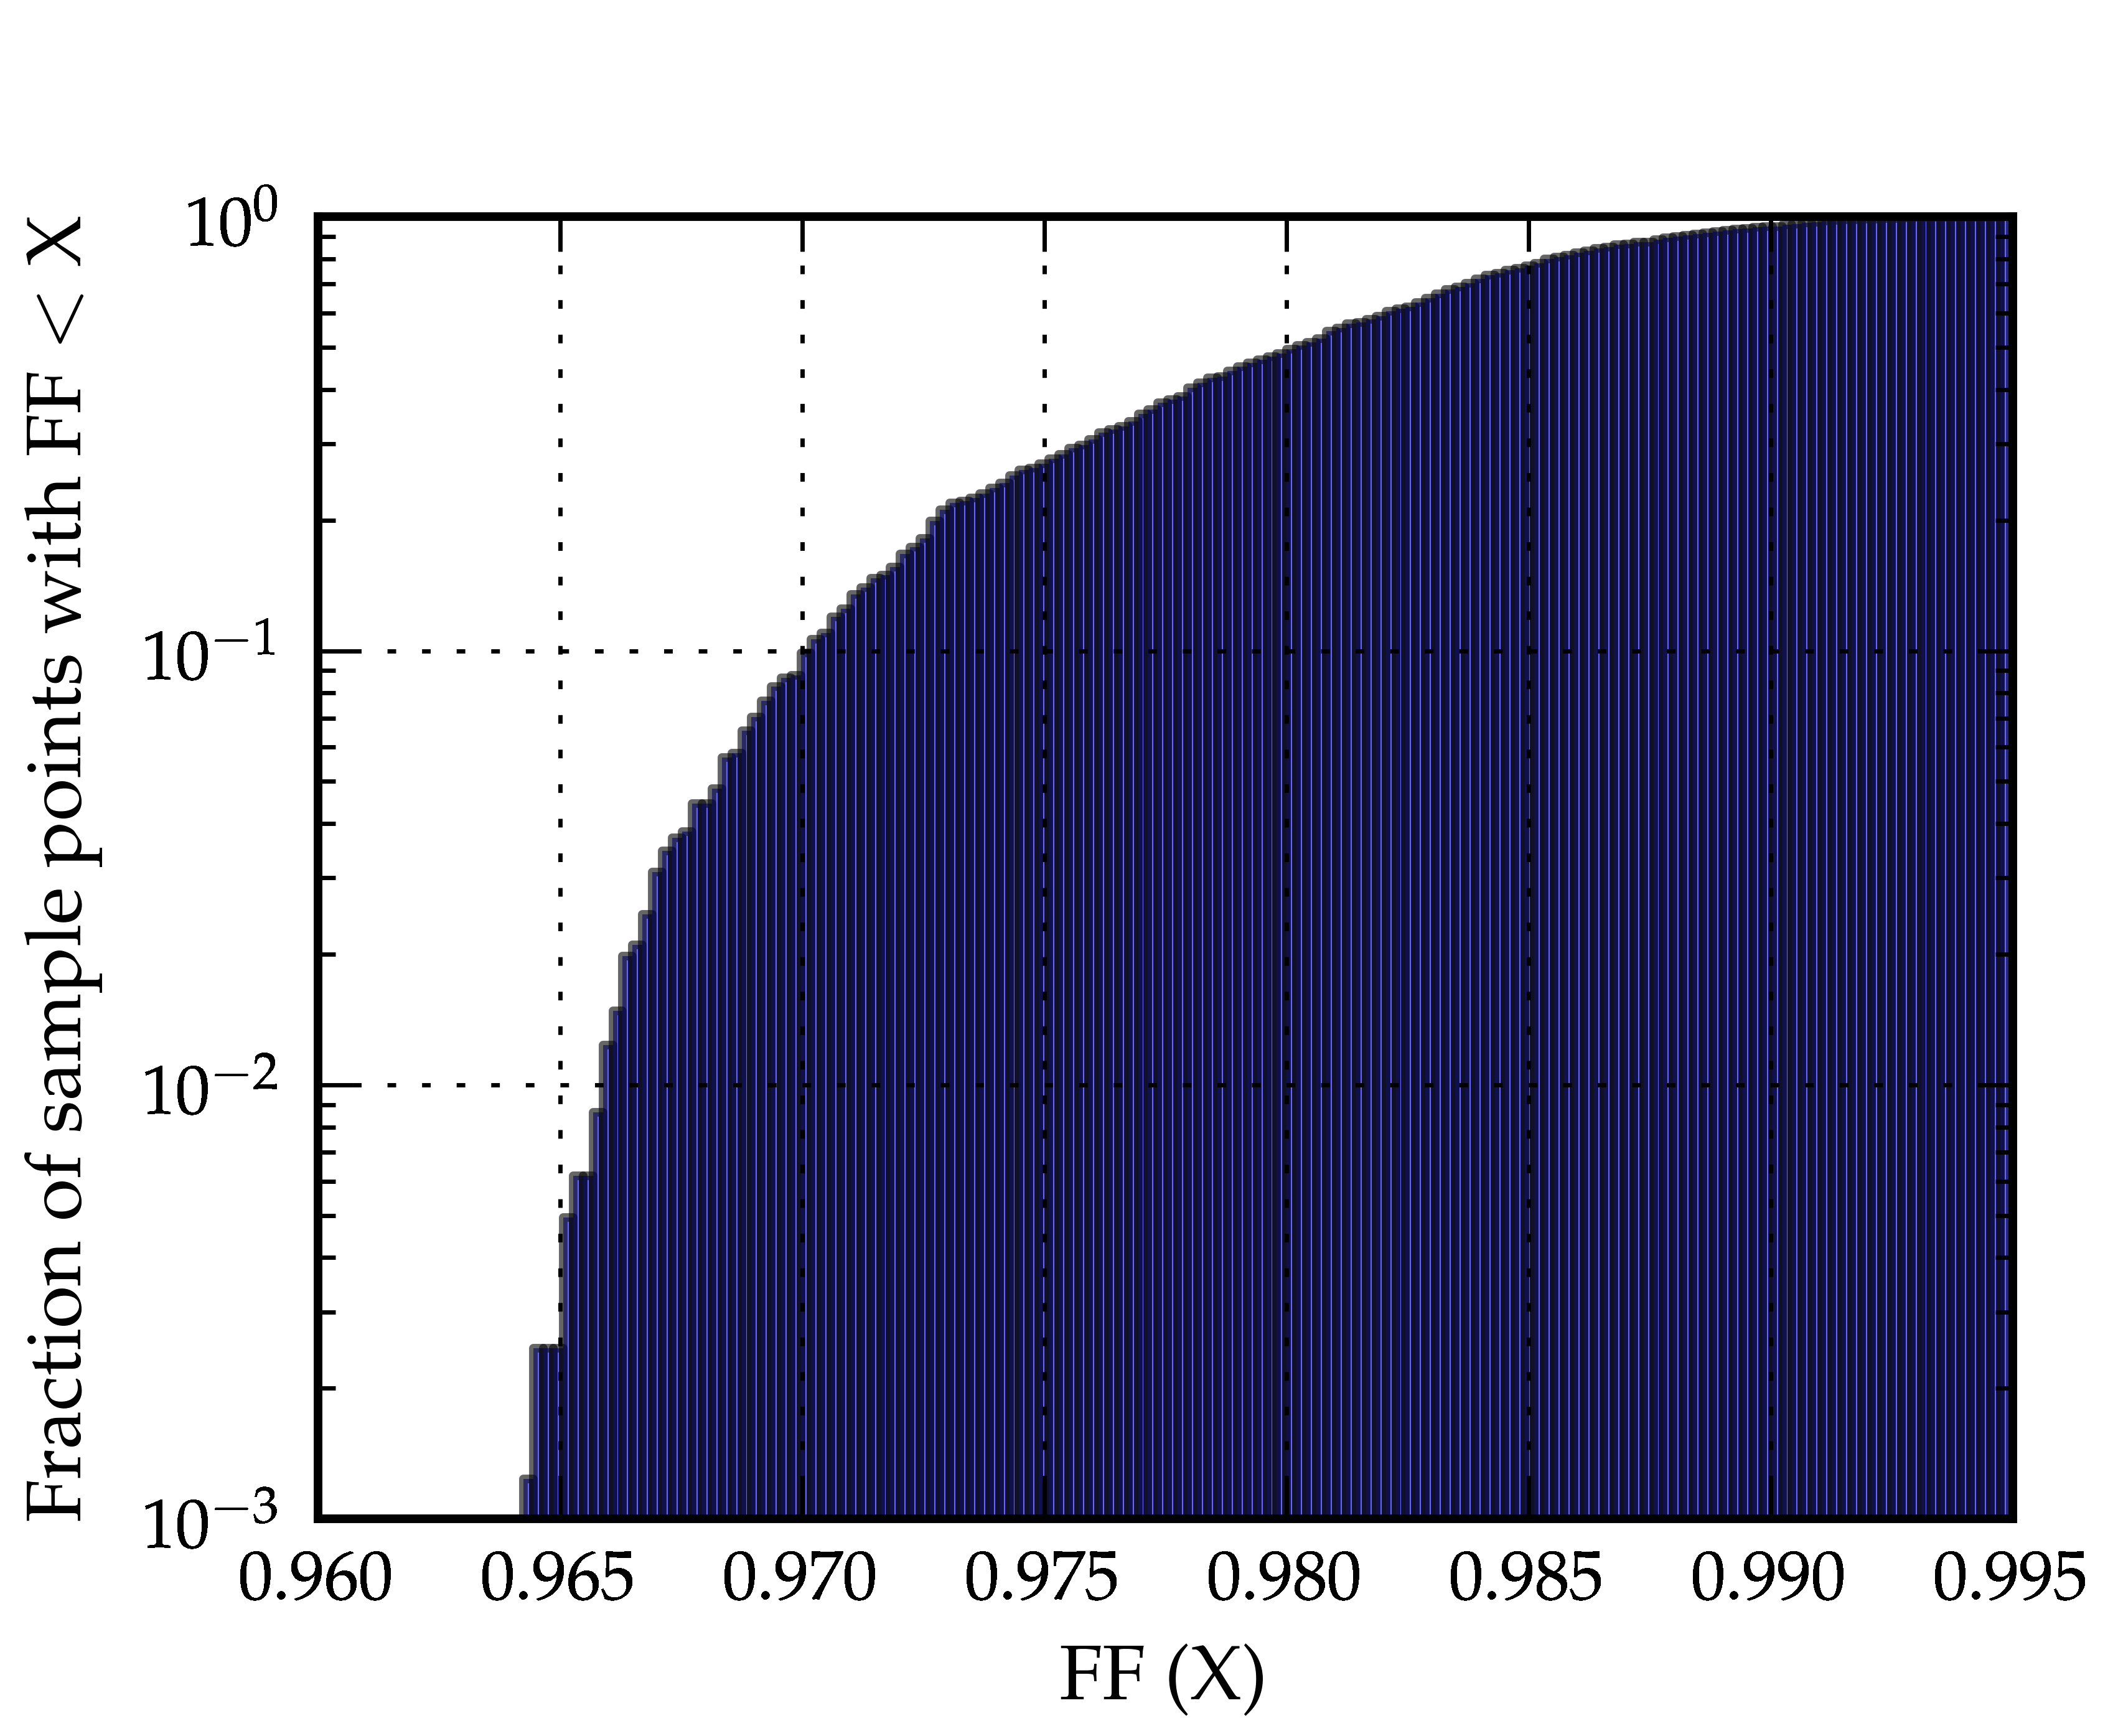
\includegraphics[scale=0.04, clip=false, totalheight=0.3\textheight, width=\columnwidth]{EOB22vsF2cutcumhist12.png}
\caption{\label{fig:cumhist_f2eob22_cut12}This figure shows the cumulative histogram of the the fitting factors of a bank of Taylor F2 waveforms against the inspiral-merger-ringdown EOB waveforms, with only the dominant multipole. The points shown here cover only the component mass region with total masses below $12M_{\odot}$.}
\end{figure}

\begin{figure}
\centering
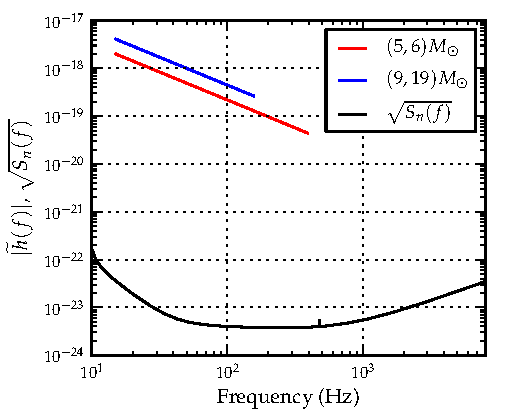
\includegraphics[scale=0.04, clip=false, totalheight=0.3\textheight, width=\columnwidth]{fd_fd_psd.pdf}
\caption{\label{fig:F2waveformsM}This figure shows the (scaled) amplitude of the frequency domain waveforms for BBH with total mass $11M_{\odot}$ (red) and $28M_{\odot}$ (blue), starting at the time when the frequency of the emitted GW is $15Hz$. The component masses of each system are shown in the label. Also shown is the Zero-Detuned-High-Power noise power-spectral-density (PSD) estimate of the detector $S_n(f)$. Lower values of the PSD indicate higher sensitivity of the detector at that frequency. This figure illustrates that BBH systems with lower masses have relatively more waveform cycles in the most sensitive frequency range of the detector.}
\end{figure}

\begin{figure*}[]
\centerline{
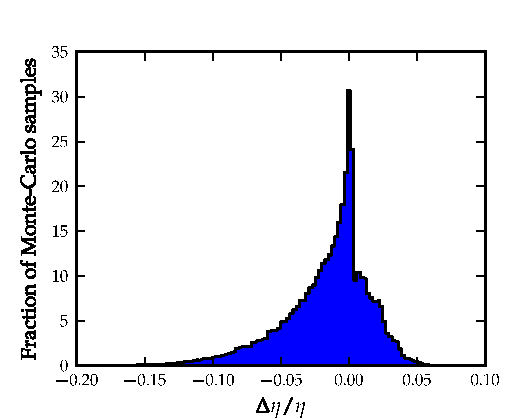
\includegraphics[scale=0.04, clip=false,keepaspectratio=true, width=\columnwidth]{hist_eta_err14paramF2EOB.pdf}\label{fig:errparams_f2eob_eta}              
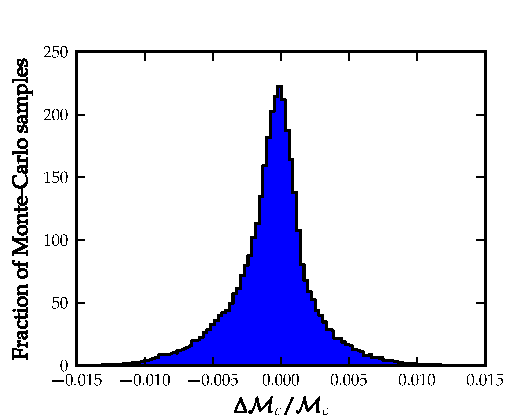
\includegraphics[scale=0.04, clip=false, keepaspectratio=true, width=\columnwidth]{hist_mchirp_err14paramF2EOB.pdf}\label{fig:errparams_f2eob_mchirp}
}
\caption{This figure shows the histogram of fractional difference between the physical parameters of each sampled point and those corresponding to the waveform in the Taylor F2 template bank that had the highest overlap with the inspiral-merger-ringdown EOB waveform generated for the sample point. The left plot shows the fractional difference in the symmetric mass ratio $\eta$ and the right plot shows the fractional difference in the chirp mass $\mathcal{M}_c= (m_1m_2)^{3/5}(m_1+m_2)^{2/5}$. The component-mass-space region shown here is the entire BBH region with individual component-masses in $(3-25)M_{\odot}$.}
\label{fig:errparams_f2eob}
\end{figure*}

%\begin{figure}
%\centering
%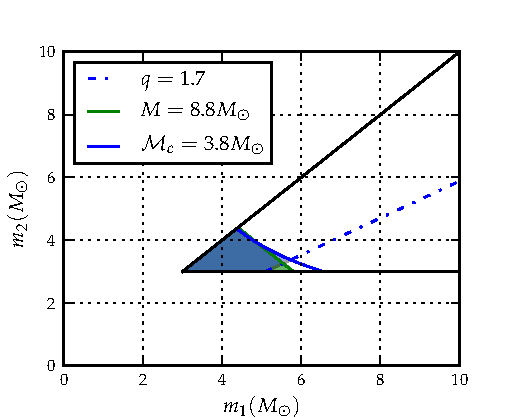
\includegraphics[scale=0.04, clip=false, totalheight=0.3\textheight, width=\columnwidth]{f2EffectualArea.pdf}
%\caption{\label{fig:F2EffectualArea}This figure shows the region of the stellar-mass BBH space, such that a template bank of Taylor F2 waveforms has $\FF$ above $0.965$ over $99.9\%$ of the points sampled in that region. Here, $q=m_1/m_2$ and $\mathcal{M}_c = (m_1m_2)^{3/5}M^{-1/5}$. The green shaded area corresponds to systems with $M<8.8M_{\odot}$, while the blue shaded area corresponds to systems with $\mathcal{M}_c<3.8M_{\odot}$ and $q > 1.7$. We find that for both of these regions, not more than $0.1\%$ of the sample points had a $\FF$ with the Taylor F2 template bank below $0.965$.}
%\end{figure}

We do a Monte-Carlo simulation over the entire stellar-mass BBH mass space to find regions in the component-mass space where a template bank of Taylor F2 waveforms has $\mathcal{FF}$ above $0.965 (0.947)$. The exact waveform $h^e$ is approximated by the EOBNRv2HM waveform model which sums over five dominant and sub-dominant waveform multipoles (i.e. $h_{22},h_{21},h_{33},h_{44}\&h_{55}$) to construct the final waveform.
The simulation was done by sampling 99,000 systems over the designated region of the component-mass space, uniformly distributed in individual component-mass. These systems were also uniformly distributed in sky-location angles and inclination and polarization angles, which appear in the detector's response function towards the GW signal \citep{Sathyaprakash:2009xs}. For each of these points, we generate the EOBNRv2HM waveform for the system with component masses given by the coordinates of the point, starting from the time when the gravitational-wave frequency from the system crosses 15Hz, and ending when the quasi-normal ringing of the final black-hole (formed by the coalescence of the binary) ends. Next, we generate a bank of 3.5PN Taylor F2 waveforms, gridded using the 2PN Owen-Sathya bank placement metric \citep{OwenTemplateSpacing,SathyaBankPlacementTauN,SathyaMetric2PN} to cover the same mass region. This bank is generated with the requirement that $\MM=0.97$. We record the $\mathcal{FF}$ of the 
template bank at all the Monte-Carlo points.

Fig.~\ref{fig:match_f2eob_f2eob22_all} (left) shows the $\mathcal{FF}$ of the Taylor F2 template bank at each point in the component-mass space. We observe a distinct region of the component-mass space where the $\mathcal{FF}$ of the bank is higher than $0.965\, (0.947)$. To explore in detail the region of the space with total-mass below $8.8M_{\odot} (14M_{\odot})$, in Fig.~\ref{fig:cumhist_f2eob_cut14} we show (on the y-axis) the relative fraction of the component-mass-space region (with total-mass below $8.8M_{\odot} (14M_{\odot})$) over which the Taylor F2 waveform template bank has $\mathcal{FF}$ below or equal to the corresponding value on the x-axis. It was found that the $\FF$ of the Taylor F2 bank evaluated to be greater than or equal to $0.965\, (0.947)$ at more than $99.9\%$ of the sampled points in these regions, respectively. It is expected that systems with lower total mass can be detected using Taylor F2 banks, as lower total mass implies that the inspiral phase lasts longer in the sensitive 
frequency band 
of the detector. And as PN theory describes this phase of the evolution accurately, this decreases the relative importance of the missing merger-ringdown waveform cycles in the PN waveform. This is illustrated in Fig.~\ref{fig:F2waveformsM}, which shows gravitational waveforms for two BBH systems in the frequency domain, modeled using the Taylor F2 model. We see that as the total mass of the system decreases, it has more inspiral waveform cycles in the sensitive frequency band of the detector. 

In Fig.~\ref{fig:errparams_f2eob}, we show a histogram of the fractional differences between the true physical mass parameters of a system and the mass parameters of the template waveform in the Taylor F2 bank that had the maximum value of maximized overlap with the EOBNRv2HM waveform for that system. In other words, it shows the fractional error in the mass parameters recovered using a bank of Taylor F2 waveform templates. The mass-coordinates used to show the errors are the dimensionless symmetric mass-ratio $\eta$, and the chirp mass $\mathcal{M}_c$, where
\begin{equation}
\label{eq:Mchirpdef}
\mathcal{M}_c = (m_1m_2)^{3/5}(m_1+m_2)^{2/5}.
\end{equation}
The chirp mass parameter determines the total length in time of the inspiral part of the waveform (to leading order) \citep{SathyaBankPlacementTauN} (see Eqns. [3.1-3.3] of), and the phase of the waveform is quite sensitive to it. This is also the reason why the chirp mass is recovered with greater precision, as seen in Fig.~\ref{fig:errparams_f2eob_mchirp}, as templates are packed more densely along the $\mathcal{M}_c$ axis in the bank. These figures serve the purpose of indicating that there are no accidental matches between the EOBNRv2HM and Taylor F2 waveforms with very different physical parameters, as the fractional difference between the actual physical parameters of the system and those recovered using the Taylor F2 template bank are $\lesssim 13\%$ for $\eta$ and $\lesssim 1.5\%$ for chirp mass which are not inconsistently large.

These results seem to indicate that, depending on one's tolerance for loss in the detection rate due to the combined effects of waveform model inaccuracy and coarseness of the discrete bank, a $0.97\MM$ Taylor F2 template banks can be used to search for BBH systems with total mass below $8.8M_{\odot}$ (for a tolerance of $10\%$ loss in the event observation rate) or $14M_{\odot}$ (for up to $15\%$ tolerated loss). This is one of the main results of this paper.

It is important to note here, that, there are two major differences between the template approximant and the \textit{true} signal approximant used. The template approximant, Taylor F2, describes only the inspiral phase of the process of coalescence of the binary, ignoring the merger and final ringdown phases. It also does not include the sub-leading waveform multipoles in constructing the final template waveform. Both of these features are captured by the EOBNRv2HM approximant, which we use to model the \textit{true} signal. To disentangle the effect of ignoring the (a) merger-ringdown, and (b) sub-leading waveform modes, we perform a Monte-Carlo simulation using EOBNRv2 (which ignores (b)) as the \textit{true} signal approximant. We sample the same stellar-mass BBH space with 25,000 points. For each point, we generate the EOBNRv2 waveform. The various sky-location angles and the inclination, polarization angles are drawn randomly from a uniform distribution, to obtain the waveform as observed by the 
detector. We again generate a bank of Taylor F2 waveforms over the same region, and calculate its $\FF$ for each of the sample points, against the corresponding EOBNRv2 waveform. Fig.~\ref{fig:match_f2eob_f2eob22_all} (right) shows the distribution of the $\FF$ so obtained for the Taylor F2 bank. Also, in Fig.~\ref{fig:cumhist_f2eob22_cut12} we explore the region of the BBH space with total mass $M\leq 12M_{\odot}$. We find that, the Taylor F2 template bank has $\FF$ above $\sim 0.965$ for $\geq 99.5\%$ of the points sampled in this restricted region. Compare this with Fig.~\ref{fig:cumhist_f2eob_cut14} (left), we notice that ignoring the sub-leading waveform modes in the \textit{true} waveforms, increases the $\FF$ of the Taylor F2 bank above $0.965$ for systems with $8.8M_{\odot}\leq M\leq 12M_{\odot}$. This value of the upper-limit on total-mass found here (i.e. $12M_{\odot}$) is consistant with a previous study \citep{CompTemplates2009} done with the EOBNRv1 model \citep{Buonanno:2007pf}, using an older version of the Advanced LIGO noise curve \citep{CompTemplates2009}. Also, comparing the left and right panels of Fig.~\ref{fig:match_f2eob_f2eob22_all}, we find that while ignoring the sub-leading modes in the \textit{true} waveforms increases the $\FF$ of the Taylor F2 bank all 
over the space, the increase is noticeably higher for systems with larger values of the mass-ratio $q$. Put in other words, the sub-leading waveform multipoles are found to be more important for the detection of systems which are more asymmetric in their component masses. For systems with $q$ close to unity, ignoring the merger-ringdown in templates seems to be the dominant cause for the loss in $\FF$ (and hence the SNR).

To distinguish between the loss in the $\FF$ due to the mismatch in the template and signal waveform models, and due to the coarseness of the bank itself, we also performed a Monte-Carlo simulation using a denser bank with $\MM\,=\,0.99$. We found that for systems with total masses upto $13M_{\odot}$, this dense bank of Taylor F2 waveforms had $\FF$ above the fiducial value of $0.965$. Comparing this with the range found for a $\MM\,=\,0.97$ bank, we see that for systems with total mass above $\sim 13M_{\odot}$, the effect of differences in the waveform models dominate. This also shows that at the cost of having more templates in the bank, it is possible to use the Taylor F2 3.5PN waveforms as templates, to detect systems with total masses upto $13M_{\odot}$. 


%\subsection{TaylorT4}\label{sec:level2:EffectualnessTaylorT4}
%Fig.~\ref{fig:match_t4eob_all} shows the $\mathcal{FF}$ of the Taylor T4 template bank at each point in the component-mass space. As with the Taylor F2 case, we observe a region of the component-mass space where the $\mathcal{FF}$ of the bank is above the acceptable minimum of $0.965$ \citep{WaveformAccuracy2008,WaveformAccuracy2010}. Looking in detail at the region of the space with total-masses below $12M_{\odot}$, we find that in this region, the Taylor T4 template bank has $\mathcal{FF}$ above $0.965$ over more than $99.9\%$ of the region. This is illustrated in Fig.~\ref{fig:cumhist_t4eob_cut12}, which shows the fraction of the component-mass region (with total mass below $12M_{\odot}$) where the T4 template bank has $\mathcal{FF}$ below the corresponding number on the x-axis. The histogram shows that, over no more than $0.02\%$ of the component-mass area does the $\mathcal{FF}$ of the T4 template bank drop below $0.965$.
%
%As before, in Fig.~\ref{fig:errparams_t4eob}, we show a histogram of the fractional differences between the true physical parameters of a system and the parameters of the template in the Taylor T4 bank that has the maximum value of maximized overlap with the EOBNRv2HM waveform for that system.
%This illustrates that there are no accidental matches of the EOBNRv2HM and Taylor T4 waveforms with very different physical parameters, as the fractional difference between the actual physical parameters of the system and those recovered using the Taylor T4 template bank, which are $\lesssim 4\%$ for $\eta$ and $\lesssim 0.1\%$ for chirp mass, are within expected bounds [citation].

\subsection{EOBNRv2 Bank}\label{sec:level2:EffectualnessEOBNRv2}
\begin{figure}
\centering
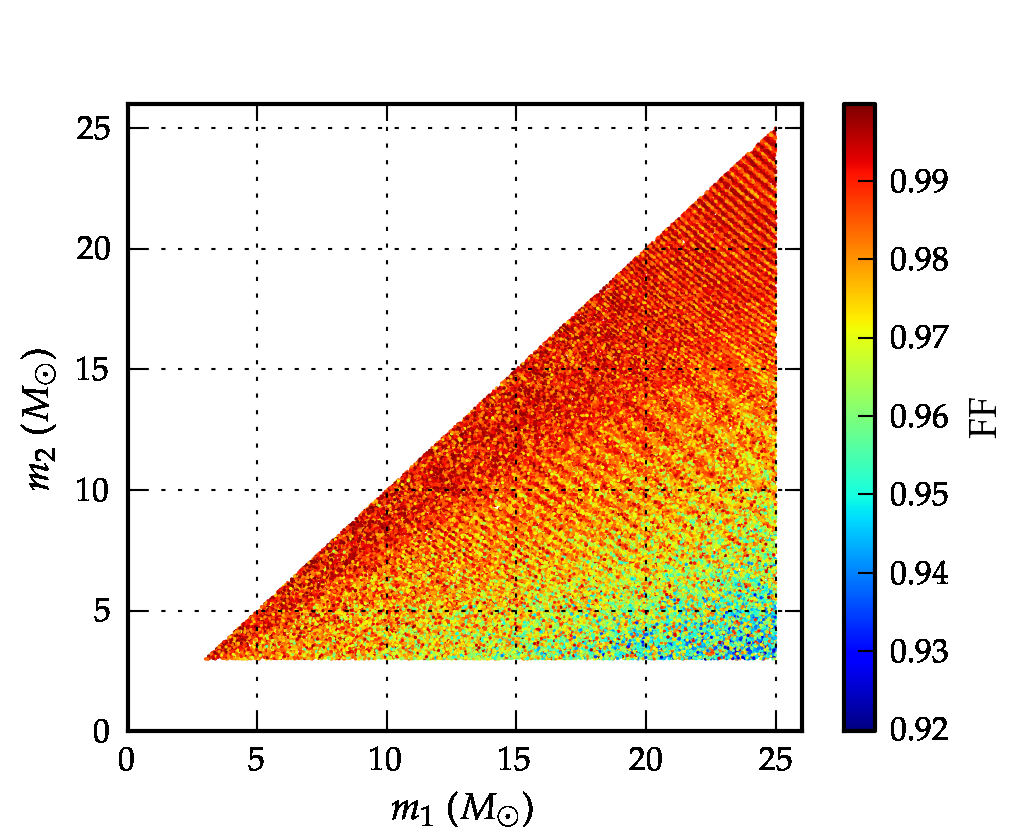
\includegraphics[scale=0.04, clip=false, totalheight=0.3\textheight, width=\columnwidth]{EOBHMvsEOB22FULLNolines.png} % XXX large figure
\caption{\label{fig:match_eob22eobhm_m1m2}This figure shows the $\FF$ of a bank of EOBNRv2 waveforms, constructed with a minimal match of 0.97 at each point in the stellar-mass BBH component-mass region. The color at each point is the value of the $\FF$ of the EOBNRv2 bank at that point against EOBNRv2HM signals.}
%The line shown on the figure demarcates (from one side) the region with $m_1/m_2>3/2\, (3.25)$. For at least $99.9\%$ of the points sampled in the regions bound by these lines, the $\FF$ of the EOBNRv2 waveform template bank is above the fiducial threshold of $0.965$ and $0.947$ respectively.
\end{figure}
\begin{figure}
\centering
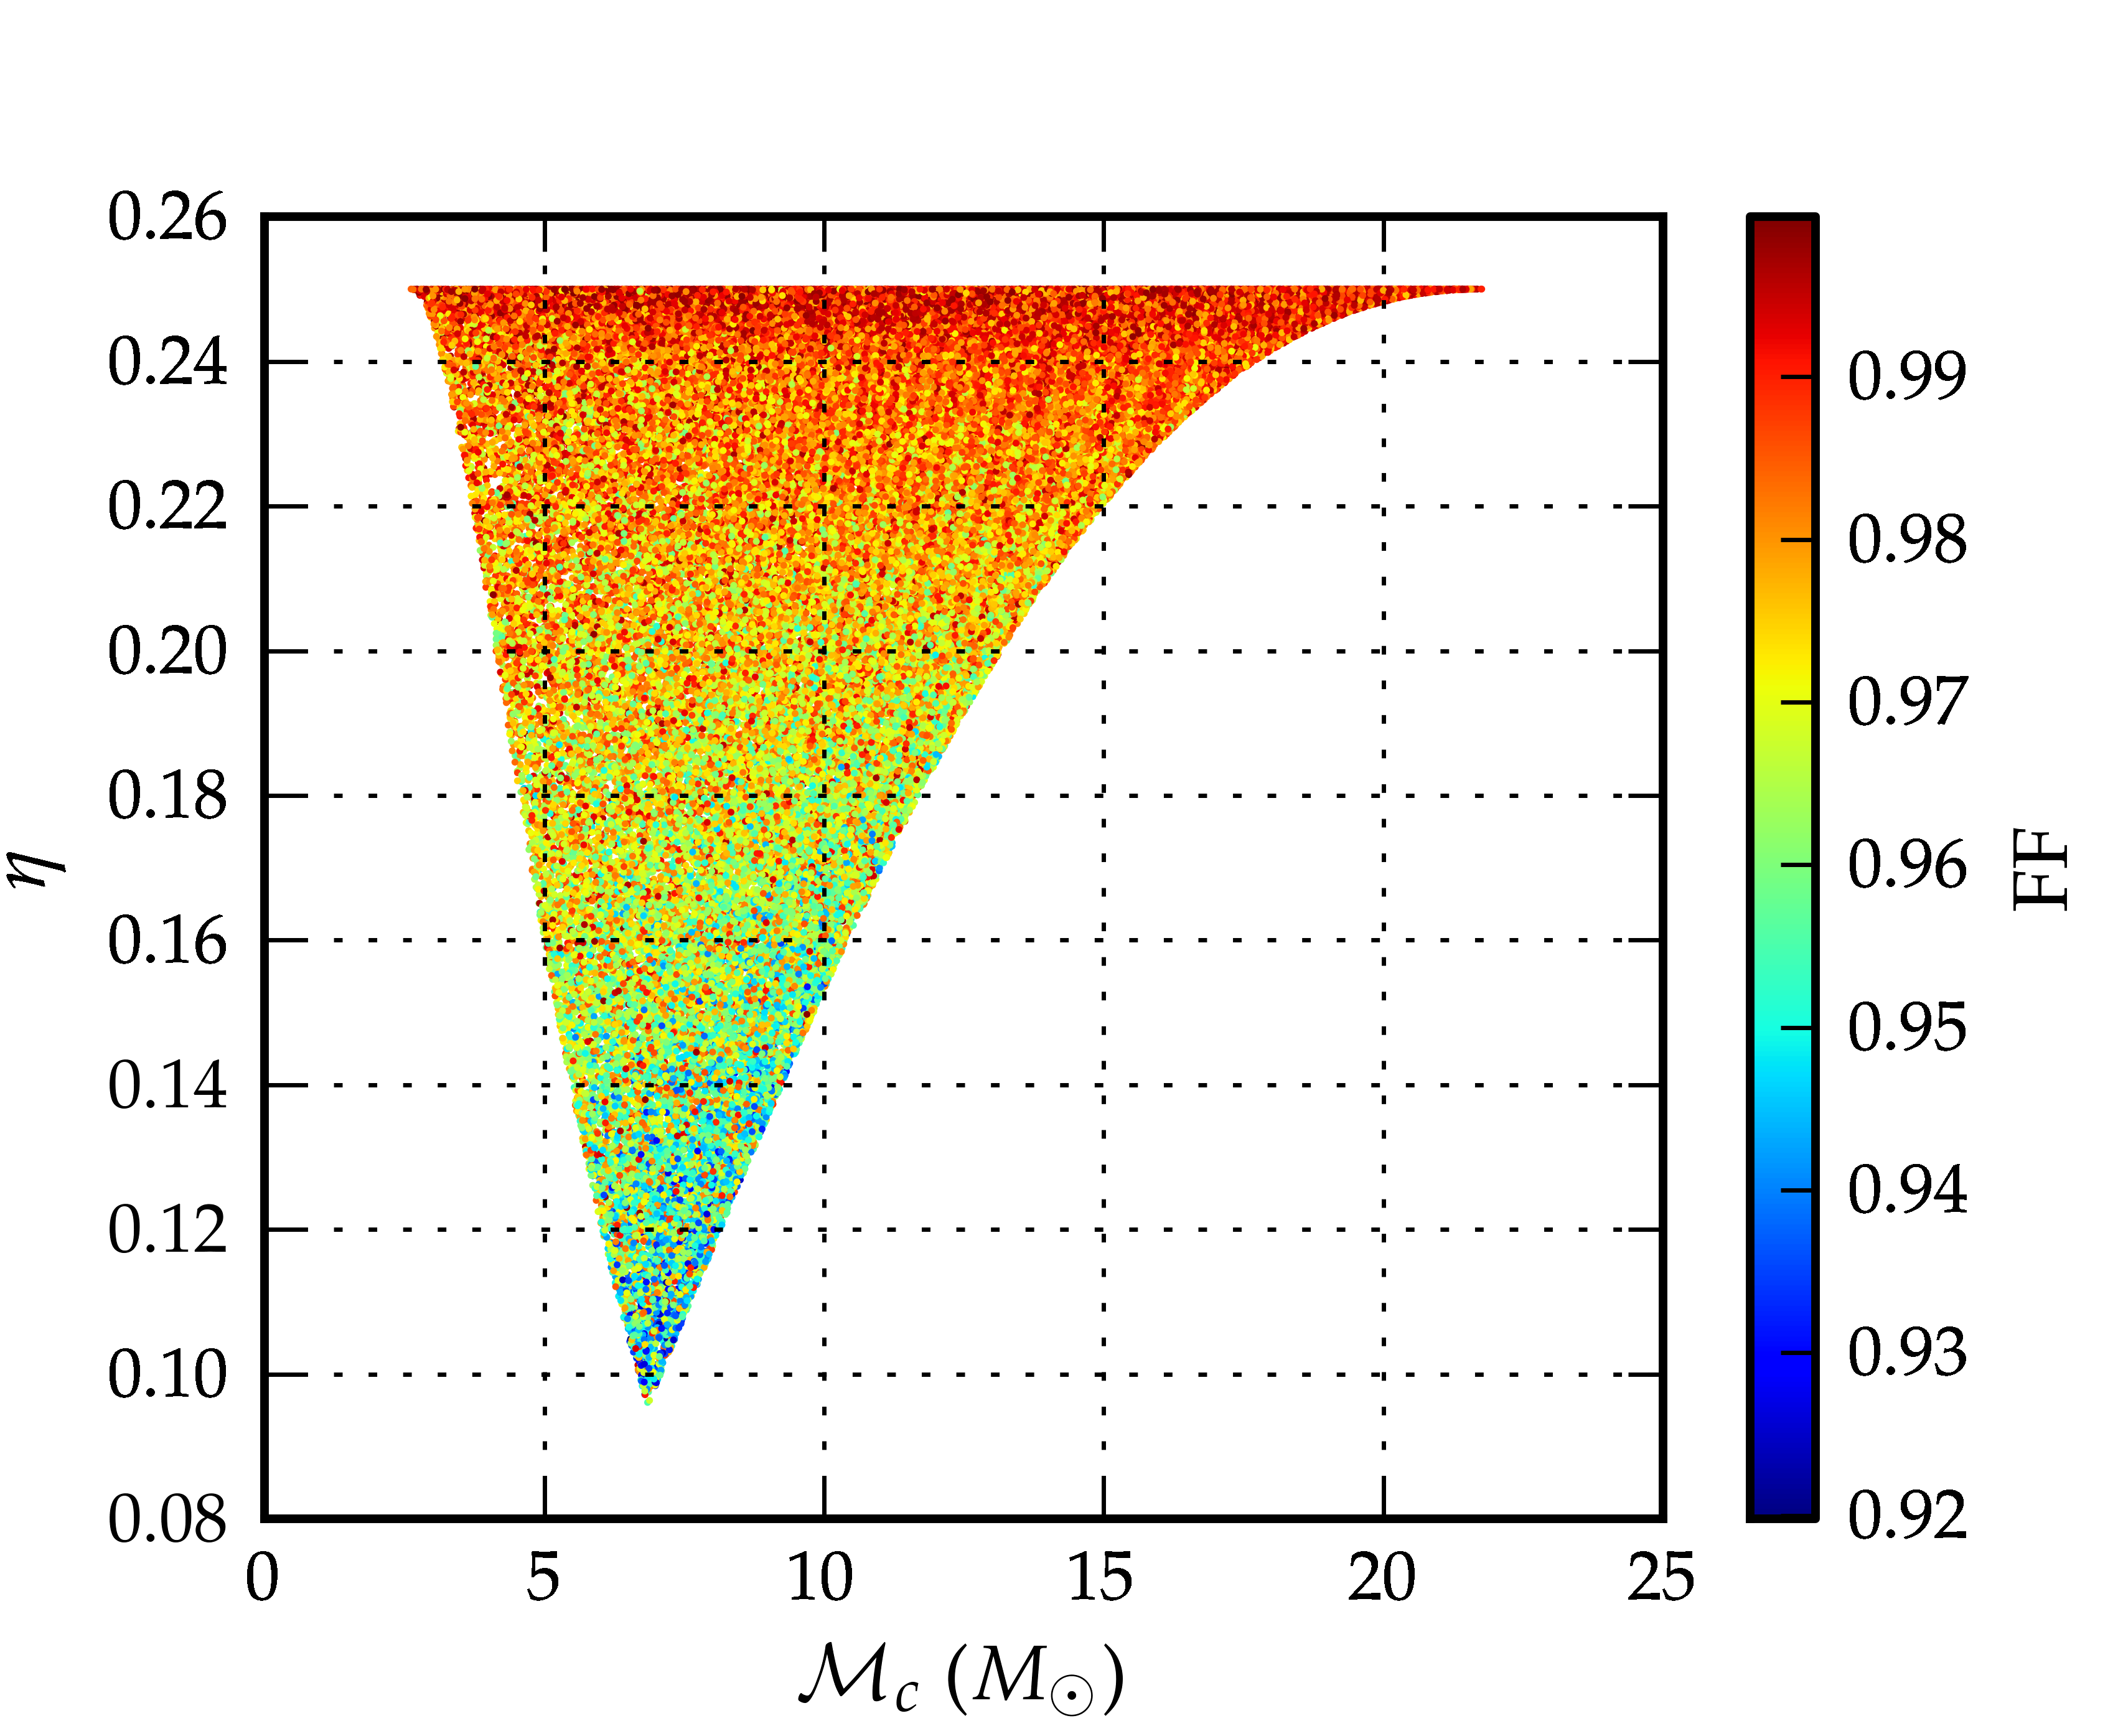
\includegraphics[scale=0.04, clip=false, totalheight=0.3\textheight, width=\columnwidth]{EOBHMvsEOB22McEtaNolines.png} % XXX large figure
\caption{\label{fig:match_eob22eobhm_mceta}This figure is the same as
Fig.~\ref{fig:match_eob22eobhm_m1m2}, but on the $\mathcal{M}_c-\eta$ axes.}
%The line in the figure demarcates the region with $m_1/m_2 < 1.5$ (green) and
%$m_1/m_2 < 3.25$ (blue).
\end{figure}
\begin{figure*}
\centerline{
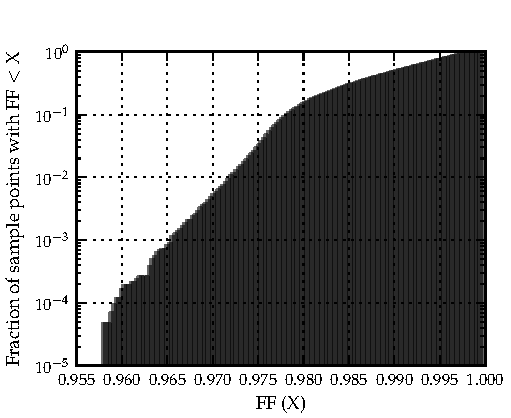
\includegraphics[scale=0.04, clip=false,keepaspectratio=true, width=\columnwidth]{EOBHMvsEOB22cutcumhist1-5.pdf}
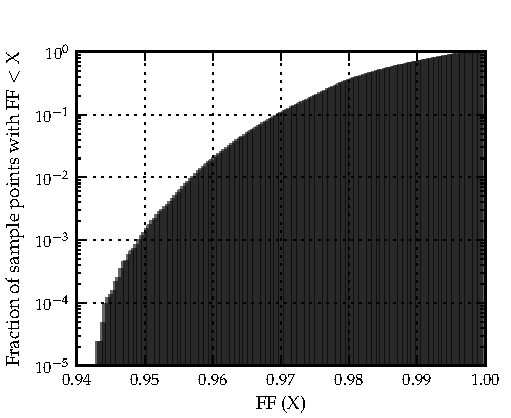
\includegraphics[scale=0.04, clip=false, keepaspectratio=true, width=\columnwidth]{EOBHMvsEOB22cutcumhist3-25.pdf}
}
\caption{\label{fig:cumhist_eob22eobhm_cuteta23}This figure shows the cumulative histograms of the fraction of the component-mass region, where the bank of EOBNRv2 waveforms has $\FF$ less than the respective values on the x-axis. The component-mass region shown here is restricted to systems with $m_1/m_2>3/2$ (left) and with $m_1/m_2>3.25$ (right).}
\end{figure*}
\begin{figure}
\centering
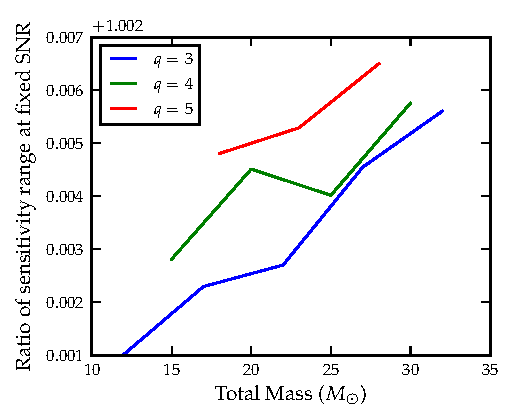
\includegraphics[scale=0.04, clip=false, totalheight=0.3\textheight, width=\columnwidth]{RatioOfSigsHM22.pdf}
\caption{\label{fig:RatioOfRangesHM22}The expectation value of SNR for a signal, when the template matches the signal exactly, is given as $\left\langle\rho^2\right\rangle = (h|h)$, where $h$ is the gravitational-waveform emitted by the system. For a system located face-on over the detector, $\left\langle\rho^2\right\rangle_{22} \simeq (h_{22}|h_{22})$ is the expected SNR from a detection search done using EOBNRv2 waveforms, and $\left\langle\rho^2\right\rangle_{HM} = (h_{HM}|h_{HM})$ is the expected SNR from a search done using EOBNRv2HM waveforms. As the name suggests, $h_{22}$ is the gravitational waveform emitted by the system modeled using EOBNRv2, while $h_{HM}$ is the waveform from the same system, at the same physical distance, modeled using EOBNRv2HM. In this figure we plot the ratio $\sqrt{\left\langle\rho^2\right\rangle_{HM}/\left\langle\rho^2\right\rangle_{22}}$ as a function of the total mass of the binary. The three lines are for different values of the mass ratio $q$. Each system is located at 
the same physical distance and has an inclination angle of $\pi/6$. At a fixed SNR, this is the same as the ratio of $D_{HM}/D_{22}$, where $D_{HM}$ and $D_{22}$ are the physical distances at which the system would be located to be detected with the same SNR in the two searches using EOBNRv2HM and EOBNRv2 templates, respectively.}
\end{figure}
\begin{figure*}[]
\centerline{
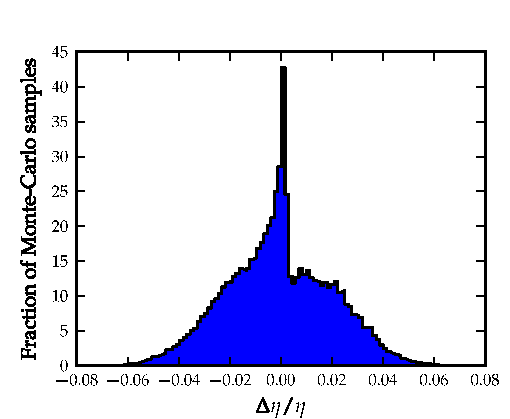
\includegraphics[scale=0.04, clip=false,keepaspectratio=true, width=\columnwidth]{hist_eta_errparamEOBHMEOB22.pdf}\label{fig:errparams_eob22eobhm_eta}              
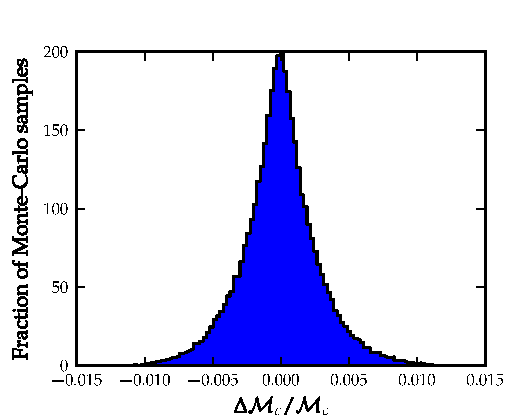
\includegraphics[scale=0.04, clip=false, keepaspectratio=true, width=\columnwidth]{hist_mchirp_errparamEOBHMEOB22.pdf}\label{fig:errparams_eob22eobhm_mchirp}
}
\caption{This figure shows the histogram of fractional difference between the physical parameters of each sampled point and those corresponding to the waveform in the EOBNRv2 template bank that had the highest overlap with the inspiral-merger-ringdown EOB waveform generated for the sample point. The left plot shows the fractional difference in the symmetric mass ratio $\eta$ and the right plot shows the fractional difference in the chirp mass $\mathcal{M}_c= (m_1m_2)^{3/5}(m_1+m_2)^{2/5}$. The component-mass-space region shown here is the entire BBH region with individual component-masses in $(3-25)M_{\odot}$.}
\label{fig:errparams_eob22eobhm}
\end{figure*}

In Sec.~\ref{sec:level2:EOBNRv2templateplacement} we found that the 2PN Owen-Sathya bank placement metric is sufficiently accurate a measure to place a bank of EOBNRv2 waveform templates. Now we investigate the regions of the stellar-mass BBH component-mass space in which a template bank of EOBNRv2 waveforms can be used for detection searches. Following the previous subsections we do this by calculating the $\mathcal{FF}$ of a 0.97$\MM$ EOBNRv2 template bank throughout the designated mass-parameter space. As in Sec.~\ref{sec:level2:EffectualnessTaylorF2}, we model the true GW signal with EOBNRv2HM waveforms. 

We do a Monte Carlo sampling of the component-mass space with 100,000 points, and for each system we generate the true GW signal using the EOBNRv2HM approximant. As before, these systems have a uniform distribution in various sky location angles and the inclination and polarization angles that determine the detector's sensitivity response to the system \citep{Sathyaprakash:2009xs}. For each of these \textit{true} waveforms, we calculate the $\FF$ of the entire bank of EOBNRv2 waveform templates. Fig.~\ref{fig:match_eob22eobhm_m1m2} and Fig.~\ref{fig:match_eob22eobhm_mceta} show the value of the $\FF$ of the bank of EOBNRv2 waveform templates at all sample points over the designated component-mass region. Looking in detail at the region of the space with mass-ratio $q$ above $1.5\, (3.25)$, we find that the $\FF$ of the EOBNRv2 waveform bank is above $0.965\, (0.947)$ over $99.9\%$ of this restricted region. This is illustrated in the cumulative histograms shown in Fig.~\ref{fig:cumhist_eob22eobhm_cuteta23} 
which show (on the y-axis) the fraction of the bank (over the restricted region with $q$ above $1.5$ (left) and $3.25$ (right)) that has $\FF$ below the corresponding number on the x-axis. 

For BBH systems with mass ratio $q$ quite close to unity, the amplitude of the sub-leading waveform multipoles is orders of magnitude smaller than the amplitude of the dominant $(l=2,m=2)$ multipole. As $q$ increases, the relative amplitude of the sub-leading multipoles increases. This is illustrated by Fig [1] of Ref.~\citep{BuonannoEOBv2Main}, where they plot the amplitude of the first few leading order waveform modes for binaries with mass ratio $q\,=\,\{1,6\}$. It is not surprising that we find that the $\FF$ of the EOBNRv2 bank falls below the threshold of $0.965\,(0.947)$ BBH systems that are asymmetric in component-masses with $q\geq 1.5\, (3.25)$. These results look promising in the sense that over a significant portion of the stellar-mass BBH space, the leading-order EOB waveform is quite sufficient to be used to detection purposes. The loss in recovered SNR, because of ignoring higher-order modes and the coarseness of the template bank, doesn't go above $10\%-15\%$ over a significant portion of the 
space. To estimate the effect of using templates without higher-order modes on the BBH range that the search would be sensitive to, we calculate the ratio of the average SNR that detection searches would detect from face-on BBH systems that are located at the same distance, if they use EOBNRv2HM templates to that if they use EOBNRv2 templates. For different values of the mass-ratio $q$, this is shown in Fig.~\ref{fig:RatioOfRangesHM22}. This is the same as the ratio of the distances that detection searches would be sensitive to, at a fixed SNR, depending on whether they do or do not ignore the higher-order modes. This hints that there is a possibility of gaining $\sim 0.5\%$ in the range of sensitivity for BBHs with $q\gtrsim 3.25$, by using EOBNRv2HM templates in searches. 


Fig.~\ref{fig:errparams_eob22eobhm} shows a histogram of the difference between the actual physical mass parameters of a system and the mass parameters of the EOBNRv2 template with which the \textit{true} waveform had the highest overlap $\Olap$ over the entire bank. This illustrates that there are no accidental matches of the EOBNRv2HM and EOBNRv2 waveforms with very different physical parameters, as the fractional difference between the actual physical parameters of the system and those recovered using the EOBNRv2 template bank, which are $\lesssim 6\%$ for $\eta$ and $\lesssim 1\%$ for chirp mass, are not inconsistently large. 



\section{Conclusions}\label{sec:level1:conclusion}
%\begin{figure}
%\centering
%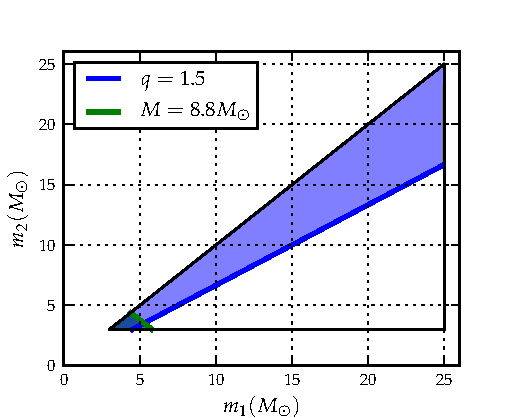
\includegraphics[scale=0.04, clip=false, totalheight=0.3\textheight, width=\columnwidth]{Massregions.pdf}
%\caption{\label{fig:ApproximantArea}In the region shaded blue, a template bank of EOBNRv2 waveforms has $\FF > 0.965$ for at least $99.9\%$ of the points sampled in the it. This region is bounded by $m_1,m_2>3M_{\odot}$ and $M<8.8M_{\odot}$. The green shaded region, similarly, is where a template bank of 3.5 Taylor F2 waveforms has $\FF > 0.965$ for at least $99.9\%$ of the points sampled in it. This region is bounded by $m_1,m_2>3M_{\odot}$ and $q < 1.5$, where $q=m_1/m_2$.}
%\end{figure}
Searches for GW signals from BBH systems involve matched-filtering the detector strain data with modeled waveforms templates as the filter. The efficiency of the filter hinges on the accuracy of the modeled waveform that is used as a filter template. In the past, 3.5PN Taylor F2 waveforms were used as templates in detection searches done with initial LIGO and Virgo \citep{Colaboration:2011nz,Abadie:2010yb,Abbott:2009qj,Abbott:2009tt,Messaritaki:2005wv}. With the increased sensitivity of the imminent second-generation detectors, the searches become more sensitive to the inaccuracy of the template waveforms. 

The detection searches are done with a discrete \textit{bank} of points, sampled over the BBH component-mass space. Owen and Sathyaprakash \citep{OwenTemplateSpacing,SathyaMetric2PN,SathyaBankPlacementTauN} derived a metric in this space that lets one place a grid of points in it \citep{BabaketalBankPlacement}, given a requirement on the maximum allowed event observation rate loss due to the coarseness of the grid. The set of waveforms generated for systems corresponding to each of the points in this bank, is called a \textit{template bank}. A caveat of this method is that this metric was derived using frequency domain PN waveforms, which included corrections to the GW phase to 2PN order. \textit{A priori}, that this will be an accurate measure for placing a template bank of leading-order $(l=2,m=2)$ EOBNRv2 waveforms is not guaranteed.

For stellar-mass BBHs with individual black hole mass ranging in $(3-25)M_{\odot}$, we study the effectiveness of the Owen-Sathya bank-placement metric in placing a bank of EOBNRv2 waveform templates. We perform large-scale Monte-Carlo investigations, calculating the $\FF$ of the EOBNRv2 template bank against EOBNRv2 waveforms as the true GW signals. We find that a bank constructed with the requirement of $\MM$ to be 0.97, actually had $\FF$ above $0.97$ for $98.5\%$ of the sampled points. The $\FF$ for this bank never fell below $0.96$. Even though the metric was only constructed for 2PN accurate frequency domain PN waveforms, its success in sufficiently covering the component-mass space with EOBNRv2 waveforms is thus remarkable. This result is significant in the sense that it shows that while using EOBNRv2 waveforms for detection searches in advanced LIGO era, the 2PN Owen-Sathya metric is quite sufficient a measure to place a bank of waveform templates.

Using detailed Monte-Carlo simulations, we show that template banks (placed using the 2PN Owen-Sathya bank-placement metric \citep{SathyaMetric2PN}) of 3.5PN restricted Taylor F2 waveforms can be used to search for gravitational waveforms from BBHs with total mass below $8.8M_{\odot}\, (14M_{\odot})$, without incurring more than a $10\%\, (15\%)$ loss in event detection rate due to template model inaccuracy and a coarse bank grid. This was studied using the criterion of Fitting Factor ($\FF$) \citep{FittingFactorApostolatos}, and we computed the $\FF$ of the Taylor F2 template bank over the entire stellar-mass BBH region of the component-mass space (Fig.~\ref{fig:match_f2eob_f2eob22_all}, left panel). We found that a template bank of Taylor F2 waveforms has $\FF$ above $0.965\, (0.947)$ for more than $99.9\%$ of the sampled BBH systems with total mass below $8.8M_{\odot}\, (14M_{\odot})$. This is expected, as lower the total mass of the BBH system, the more waveform cycles it has in the sensitive frequency 
band of the detector. 
The more the cycles that the waveform has in the sensitive band, the lesser the relative importance of the missing merger-ringdown phase in the PN approximant and of the inaccuracy of the PN waveforms during late-inspiral. The Taylor F2 bank loses $\FF$ because of not including the (a) merger-ringdown phase, and (b) sub-leading waveform modes. Using Monte-Carlo simulations, we find that ignoring (b) causes the bank to lose $\FF$ for BBH systems that are (more) \textit{asymmetric} in component masses. The lack of merger-ringdown in the templates, remains the largely dominant cause for the bank to have lower $\FF$ for the symmetric $(q\rightarrow 1)$ systems. We also find that for a more densely packed bank, with $\MM\,=\,0.99$, we get $\FF$ values above the fiducial threshold of $0.965$ for systems with total masses up to $13M_{\odot}$. This implies that at the cost of having more templates (almost by a factor of $2$) in the bank, Taylor F2 waveforms can be used in detection searches for systems with total mass up to $13M_{\odot}$. This is in agreement with earlier results \citep{CompTemplates2009}, obtained using the EOBNRv1 waveform model \citep{Buonanno:2007pf} and an older version of the Advanced LIGO noise curve.

Also, we determine the portion of the stellar-mass BBH space where an EOBNRv2 template bank is sufficient for detection searches and to investigate the loss in SNR incurred by ignoring higher-order waveform multipoles in the templates. We do the exact same study as we did for the Taylor F2 waveform template bank, modeling the true GW signals with EOBNRv2HM waveforms. We find that such a template bank can viably be used to search for GW signals from BBH systems with mass-ratio in the range $1\leq q\leq 1.5 (3.25)$ (Fig.~\ref{fig:match_eob22eobhm_m1m2},~\ref{fig:match_eob22eobhm_mceta}), with lesser than $10\, (15)\%$ loss in the detection rate. For systems with $q\gtrsim 3.25$, there is a possibility of gaining sensitivity range by using EOBNRv2HM templates. This is an expected result since for BBH systems with $q$ close to unity, the gravitational waveform can be approximated by the leading order $(l=2,m=2)$ EOB waveform multipole. This is because for such systems the sub-leading order waveform multipoles 
have amplitudes that are much weaker than the amplitude of the leading waveform multipole. This is illustrated in Fig.[1] of Ref.~\citep{BuonannoEOBv2Main}.

Our results suggest that a significant portion of the stellar-mass BBH systems can be searched for using existing iLIGO-style infrastructure. For systems with total mass below $8.8M_{\odot}-14M_{\odot}$ and q between unity and $1.25\,-\,3.25$, detection searches can use $0.97\MM$ template banks of Taylor F2 and EOBNRv2 waveforms (respectively) without more than a $10\%-15\%$ loss in event observation rate due to waveform inaccuracy and coarseness of the discrete bank grid. For BBHs with total mass greater than $14M_{\odot}$ and mass ratio $q> 3.25$, searching with template banks of either of Taylor F2 or EOBNRv2 could lead to higher than $15\%$ loss in detection rate due to these factors. As this study uses the fitting factor which normalizes out the source distance, the bias due to the detectors being sensitive to face-on systems further away than edge-on systems is not taken into account here \citep{LarneHMStudyDL}. Work would be required in the future to be able to incorporate higher waveform modes into 
the detection searches \citep{HigherHarmonicsDAsearch}; to extend this study for systems with spinning and/or precessing BHs; and to possibly extend these results for GW signals in real detector noise, folding in the effect of waveform-based noise-trigger elimination methods \citep{Allen:2004gu}.

% If in two-column mode, this environment will change to single-column
% format so that long equations can be displayed. Use
% sparingly.
%\begin{widetext}
% put long equation here
%\end{widetext}

% figures should be put into the text as floats.
% Use the graphics or graphicx packages (distributed with LaTeX2e)
% and the \includegraphics macro defined in those packages.
% See the LaTeX Graphics Companion by Michel Goosens, Sebastian Rahtz,
% and Frank Mittelbach for instance.
%
% Here is an example of the general form of a figure:
% Fill in the caption in the braces of the \caption{} command. Put the label
% that you will use with \ref{} command in the braces of the \label{} command.
% Use the figure* environment if the figure should span across the
% entire page. There is no need to do explicit centering.

% \begin{figure}
% \includegraphics{}%
% \caption{\label{}}
% \end{figure}

% Surround figure environment with turnpage environment for landscape
% figure
% \begin{turnpage}
% \begin{figure}
% \includegraphics{}%
% \caption{\label{}}
% \end{figure}
% \end{turnpage}

% tables should appear as floats within the text
%
% Here is an example of the general form of a table:
% Fill in the caption in the braces of the \caption{} command. Put the label
% that you will use with \ref{} command in the braces of the \label{} command.
% Insert the column specifiers (l, r, c, d, etc.) in the empty braces of the
% \begin{tabular}{} command.
% The ruledtabular enviroment adds doubled rules to table and sets a
% reasonable default table settings.
% Use the table* environment to get a full-width table in two-column
% Add \usepackage{longtable} and the longtable (or longtable*}
% environment for nicely formatted long tables. Or use the the [H]
% placement option to break a long table (with less control than 
% in longtable).
% \begin{table}%[H] add [H] placement to break table across pages
% \caption{\label{}}
% \begin{ruledtabular}
% \begin{tabular}{}
% Lines of table here ending with \\
% \end{tabular}
% \end{ruledtabular}
% \end{table}

% Surround table environment with turnpage environment for landscape
% table
% \begin{turnpage}
% \begin{table}
% \caption{\label{}}
% \begin{ruledtabular}
% \begin{tabular}{}
% \end{tabular}
% \end{ruledtabular}
% \end{table}
% \end{turnpage}

% Specify following sections are appendices. Use \appendix* if there
% only one appendix.
%\appendix
%\section{}
%\FloatBarrier

%
%\section{EOB: Gain in Search Volume}\label{sec:level1:SearchVolume}
%We compare the sensitivity of matched-filtering searches, in terms of the effective observation volume available to them, using the different waveform approximants described in the Sec.\ref{sec:level1:PNApproximants}. One can think of the effective observation volume as the (effective) spacial volume centered at the gravitational wave detector, within which, all binary systems emitting gravitational radiation will be detected with a signal-to-noise ratio (SNR) higher than $8$, by the matched-filter. In the advanced detector era, it is expected that we will be able to observe gravitational wave signals from stellar-mass binary-black-holes (with individual component-mass ranging in $(3-20)M_{\odot}$) upto distances of $\sim1GPc$ \citep{LSCCBCRates2010}. At such distances, we can take the distribution of the sources in the sky as isotropic and homogenous [citation]. With such a distribution of sources, the effective observation volume becomes a direct measure of the event observation rate.
%
%To elucidate what we are doing, lets start with the definition of the frequency weighted dot product (overlap) between two gravitational waveforms $h_1$ and $h_2$,
%\begin{equation}\label{eq:overlap}
%(h_1|h_2) = 2\int^{\infty}_0\dfrac{\tilde{h}_1^*(f)\tilde{h}_2(f) + \tilde{h}_1(f)\tilde{h}_2^*(f)}{S_n(f)}\D f,
%\end{equation}
%where $S_n(f)$ is the Zero-Detuned-High-Power power spectral density estimate for advanced LIGO [citation], and $\tilde{h}(f) = \int^{\infty}_{-infty}exp(-2\pi\ii ft)h(t)\D t$ is the Fourier transform of the waveform $h(t)$. The factor of $S_n(f)$ gives more weight to the frequencies which advanced LIGO will be more sensitive  to, and lesser weight to the frequencies where its sensitivity would be less. This dot product (overlap), when normalized by the suitable norms of the two waveforms gives the normalized overlap between the two waveforms,
%\begin{equation}
%(\hat{h}_1|\hat{h}_2) = \dfrac{(h_1|h_2)}{\sqrt{(h_1|h_1)(h_2|h_2)}}.
%\end{equation}
%This normalized overlap would be sensitive to the relative phase of coalescence $\phi_c$ and time of coalescence $t_c$ between the two waveforms $h_1$ and $h_2$. These two parameters ($\phi_c$ and $t_c$) are extrinsic to the binary system that is the source of the gravitational waves, and so we maximize over them to get the maximized normalized overlap $\Olap$,
%\begin{equation}\label{eq:maxnormolap}
%\Olap(h_1,h_2) = \underset{\phi_c,t_c}{max}\,\l(\hat{h}_1|\hat{h}_2(\phi_c,t_c)\r),
%\end{equation}
%that gives a measure of how close the two waveforms are in the waveform manifold. The mismatch $\mathrm{M}$ between the same two waveforms can hence be written as,
%\begin{equation}\label{eq:mismatch}
%\mathrm{M}(h_1,h_2) = 1 - \Olap(h_1,h_2).
%\end{equation}
%\newline
%In a matched-filtering search, a segment of detector data $s(t)$, is matched with a template waveform $h(t)$ to give the signal-to-noise-ratio (SNR) $\rho$ as the output of the filter,
%\begin{equation}\label{eq:SNR}
%\rho = \underset{\phi_c,t_c}{max} \dfrac{(s|h\l(\phi_c,t_c)\r)}{\sqrt{(h|h)}}.
%\end{equation}
%
%The gravitational wave signal produced from a coalescing black-hole-binary can be represented in the frequency domain as
%\begin{equation}\label{eq:handg}
%\tilde{h}(f) \simeq D_{\eff}^{-1} e^{-2\pi\ii ft_0+2\ii\phi_0}\tilde{g}(f),
%\end{equation}
%where $D_{\eff}$ is the \textit{effective} distance that the detector perceives the binary to be located at; $t_0$ is the coalescence time of the binary (as measured by the detector); $\phi_0$ is a fiducial reference phase; and $\tilde{g}(f)$ is the waveform template that we use to matched-filter the detector data with. $\tilde{g}(f)$ depends only on the intrinsic parameters of the binary system (i.e. $m_1$ and $m_2$), and is normalised to unit effective distance. The effective distance is related to the actual physical distance $D_{\phys}$ at which the binary is located as [citation]
%\begin{equation}
%D_{\eff} = \dfrac{D_{\phys}}{\sqrt{F^2_+\l(1+\cos^2\iota\r)^2/4 + F^2_{\times}\cos^2\iota}},
%\end{equation}
%where $\iota$ is the angle between the line joining the detector to the binary, and the outward normal from the surface of the Earth, at the location of the detector (i.e. the inclination angle of the binary).
%\begin{subequations}
%\begin{align}
%F_+ = \dfrac{1}{2}(1+\cos^2\theta)\cos2\Phi \cos2\Psi - \cos\theta \sin2\Phi \sin2\Psi ,\\
%F_+ = \dfrac{1}{2}(1+\cos^2\theta)\cos2\Phi \sin2\Psi + \cos\theta \sin2\Phi \cos2\Psi,
%\end{align}
%\end{subequations}
%are the antenna patterns of the detector \citep{SathyaSchutzLRR} that give the sensitivity of the detector for different angular locations in the sky; and $\{\theta,\Phi,\Psi\}$ are the 3 Euler (sky) angles that are associated with the rotations that transform the frame in which the binary is in the x-y plane with its angular momentum pointing along the (+) z-axis; to the frame whose x and y axes rest along the detector's arms with the z-axis pointing outwards from the surface of the Earth.\newline
%The effective distance is a measured quantity that can be extracted from a matched-filtering search as [citation]
%\begin{equation}
%D_{\eff} = \dfrac{\sigma}{\rho};
%\end{equation}
%where $\sigma=\sqrt{(g|g)}$; and $\rho=(h|g)/\sqrt{(g|g)}$ is the SNR with which the signal $h$ will be detected using the waveform template $\tilde{g}(f)$. Note that this $\rho$ is the same as previously defined in Eq.~\eqref{eq:SNR}. Systems located in the part of the sky with $\{\iota=0,\theta=0\}$ have $D_{\eff} = D_{\phys}$. Such systems are said to be \textit{optimally oriented}. For instance, an optimally oriented binary located at $D_{\phys}=D_0$ with $\{\iota=0,\theta=0,\Phi=0,\Psi=0\}$ will have an effective distance $D_{\eff} = D_{\phys}$, whereas the same binary located at the same physical distance, but with $\{\iota=\frac{\pi}{2},\theta=0,\Phi=0,\Psi=0\}$ will have $D_{\eff} = 2D_{\phys}$. In the latter orientation, the physical distance will have to be half of what it is required to be in the former orientation, for the gravitational radiation from the binary to be detected with the same SNR. In other words, in the latter orientation the obtained SNR will be half of the SNR obtained for the 
%binary in the former orientation, keeping the physical distance the same across both cases.
%%An optimally oriented system is one that is located in the sky with an inclination angle $\iota$ with respect to the normal pointing out of the detector plane on the Earth is $0$ radians. The effective distance, we can find the actual physical distance at which the binary \textit{could} be located. Effective volume is the volume enclosed by the surface defined by the locus of the possible physical distances (which will have a spatial angular dependence) for a measured effective distance. By definition, all binaries within this spatial volume, will emit gravitaional radiation that will have a signal-to-noise ratio (SNR) $\geq 8$. We can find the radius of a sphere which has the same volume as the effective volume defined above, analytically, which will give us the effective observation volume.
%\begin{figure*}%[p]
%  \centering
%  \subfigure[$q=1$]{\label{fig:VeffsLogq1}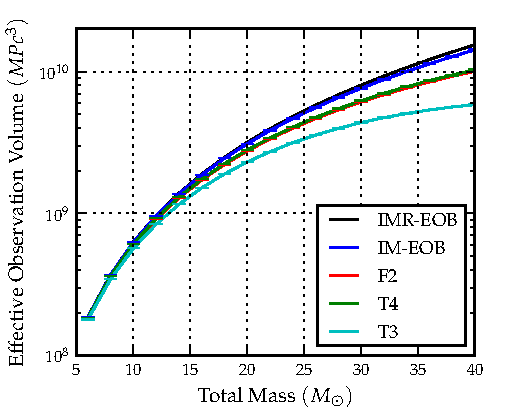
\includegraphics[scale=0.03, clip=false, height=0.28\textheight, width=\columnwidth]{Veffs_logscale_q_1_run03.pdf}}                
%  \subfigure[$q=2$]{\label{fig:VeffsLogq2}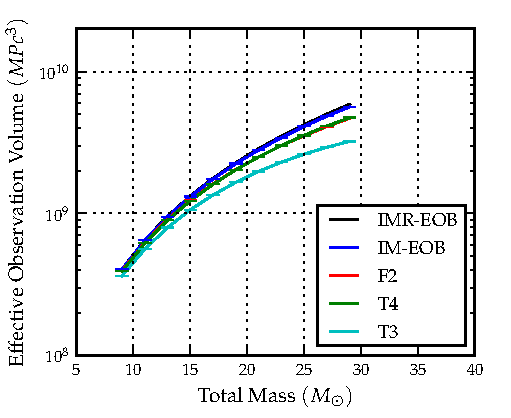
\includegraphics[scale=0.03, clip=false, height=0.28\textheight, width=\columnwidth]{Veffs_logscale_q_2_run03.pdf}}
%\\ \subfigure[$q=3$]{\label{fig:VeffsLogq3}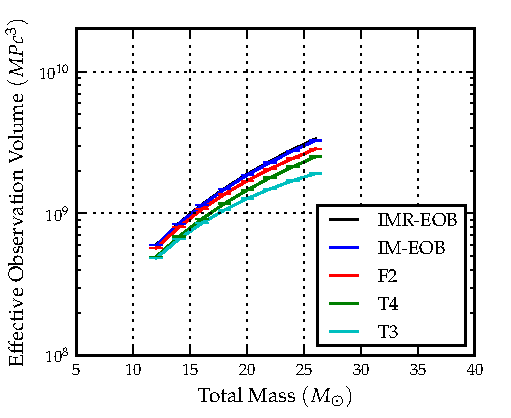
\includegraphics[scale=0.03, clip=false, height=0.28\textheight, width=\columnwidth]{Veffs_logscale_q_3_run03.pdf}}
%\subfigure[$q=4$]{\label{fig:VeffsLogq4}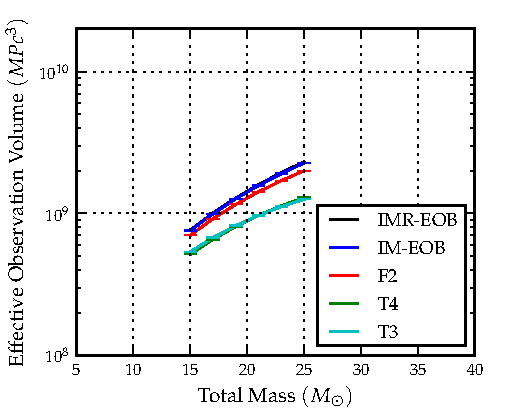
\includegraphics[scale=0.03, clip=false, height=0.28\textheight, width=\columnwidth]{Veffs_logscale_q_4_run03.pdf}}
%\\ \subfigure[$q=5$]{\label{fig:VeffsLogq5}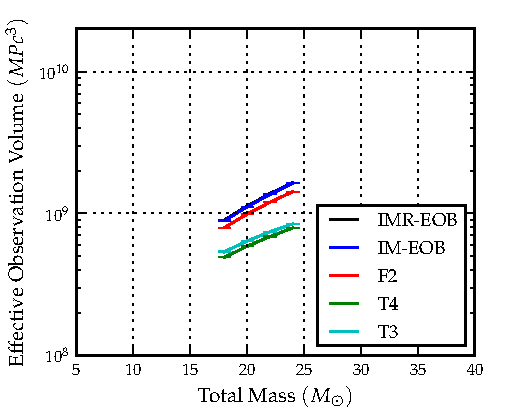
\includegraphics[scale=0.03, clip=false, height=0.28\textheight, width=\columnwidth]{Veffs_logscale_q_5_run03.pdf}}
%\subfigure[$q=6$]{\label{fig:VeffsLogq6}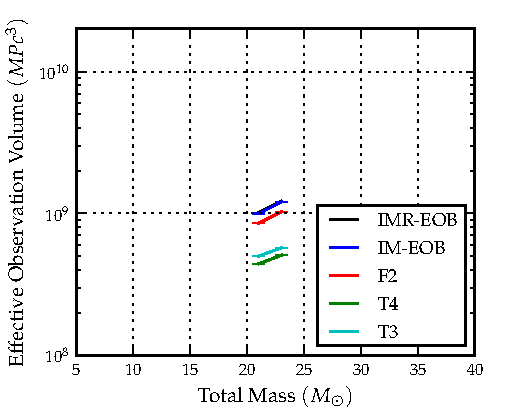
\includegraphics[scale=0.03, clip=false, height=0.28\textheight, width=\columnwidth]{Veffs_logscale_q_6_run03.pdf}}
%  \caption{These figures show the variation of the effective observation volume (logarithmic scale) with the total mass of the binary, that would be available to matched-filtering searches using different waveform approximants. Each subplot is for a different value of mass ratio $q \l(\equiv m_1/m_2\r)$.}
%  \label{fig:VeffsLog}
%\end{figure*}
%\begin{table}[h]
%\caption{\label{tab:maxTotalMassVeff} This table shows the maximum total mass of a system, for each value of the mass-ratio $q$, for which the available effective observation volume using the respective approximant is at least $90\%$ of that accesible with the full IMR EOB waveforms.}
%\begin{ruledtabular}
%\begin{tabular}{|m{0.18\columnwidth}| m{0.18\columnwidth}| m{0.18\columnwidth}| m{0.18\columnwidth}| m{0.18\columnwidth}|}
%mass-ratio & F2 & T4 & T3 & IM EOB\tabularnewline \hline
%1 & 16$M_{\odot}$ & 18$M_{\odot}$ & 10$M_{\odot}$ & 40$M_{\odot}$\tabularnewline \hline
%2 & 17$M_{\odot}$ & 17$M_{\odot}$ & - & 29$M_{\odot}$\tabularnewline \hline
%3 & 18$M_{\odot}$ & - & - & 26$M_{\odot}$\tabularnewline \hline
%4 & 19$M_{\odot}$ & - & - & 25$M_{\odot}$\tabularnewline \hline
%5 & - & - & - & 24$M_{\odot}$\tabularnewline \hline
%6 & - & - & - & 23$M_{\odot}$\tabularnewline \hline
%\end{tabular}
%\end{ruledtabular}
%\end{table}
%The furthest that a binary could be located, and be detectable with an SNR of $8$, is called the \textit{horizon distance} $D_{\horizon}$ [citation],
%\begin{equation}
%D_{\horizon}\equiv D_{\eff}(\rho = 8) = \dfrac{\sigma}{8}.
%\end{equation}
%The horizon distance defines a two-dimensional spacial surface (horizon) centered at the detector. The effective observation volume is the volume enclosed by this surface (horizon). By definition, all binaries within the effective observation volume, will emit gravitaional radiation that will have an SNR greater than $8$. Following Ref.~\citep{FinnChernoffDA} we find the radius of a sphere which has the same volume as the effective volume defined above enclosed within the horizon at SNR $8$. This is ovservation volume that we measure corresponding to the usage of different waveform approximants to model the template waveforms.\newline
%Making the assumption that the full IMR EOB model models the nature's waveforms almost perfectly \citep{EOBNRdevel01}, we calculate the horizon distance for a matched-filtering search done with IMR EOB template waveforms as
%\begin{equation}\label{eq:DhorizonEOB}
%D^{\EOB}_{\horizon} = \dfrac{\sigma^{\EOB}}{8} = \dfrac{\sqrt{(g^{\EOB}|g^{\EOB})}}{8},
%\end{equation}
%where $g^{\EOB}$ has the same meaning as in Eqn.~\eqref{eq:handg} if $\tilde{h}(f)$ is the Fourier transform of the time domain EOB waveform $h^{\EOB}(t)$. For other approximants, the horizon distance to which a match filtering search can detect using that approximant is the horizon distance the same search could detect to with the exact waveforms (approximated with IMR EOB waveforms), scaled by the fractional loss in signal-to-noise ratio due to the inherent inaccuracy of the approximant. For high SNR, the fractional loss in SNR because of the inherent inaccuracy of the waveform approximant used, is approximated by the mismatch between the waveform generated using the particular approximant and the IMR EOB waveform (for the same binary system). So, the horizon distance to which matched-filtering searches can detect gravitational wave signals to using the waveform approximant $\X$ is
%\begin{equation}\label{eq:DeffPN}
%D^{\X}_{\horizon} = D^{\EOB}_{\horizon}\times\Olap(h^{\X},h^{\EOB}),
%\end{equation}
%where $\X$ could be the Taylor T3 or the Taylor T4 or the Taylor F2 approximant of just the IM EOB waveforms; and $h^{\X}$ is the waveform generated using approximant $\X$.
%%
%%Now, to get the effective observation volume for approximant $\X$, we need to find the radius $R_{\eff}$ of the sphere, whose volume equals the volume of space that encapsulates all sources that will be detectable with $\rho\geq 8$. Ref.~\citep{FinnChernoffDA} calculates this to be (Eq.(5.1,5.2)):
%%\begin{equation}
%%\begin{split}
%%R_{\eff} = & r_0 \left[3\int_0^{\infty}\D x\,x^2 P(\rho^2(x)\geq\rho_0^2) \right]^{1/3}\\
%%\equiv & r_0 \left[3\int_0^{\infty}\D x\,x^2 P(\Gamma\geq x^2) \right]^{1/3}
%%\end{split}
%%\end{equation}
%%where $x$ is the radial parameter of the effective sphere divided by $r_0$, and $r_0$ is a fiducial distance defined in Eq.(5.2a) of Ref.~\citep{FinnChernoffDA};
%%\begin{subequations}
%%\begin{align}\nonumber
%%r_0 \equiv & \l(\dfrac{5M^{5/3}\eta f_{7/3}}{96\pi^{4/3}\rho_0^2} \r)^{1/2},\\
%%f_{7/3} = &  \int_0^{\infty}\D f \left[f^{7/3} S_n(f) \right]^{-1},\\
%%\Gamma = & 16\left[F^2_+\l(1+cos^2\iota\r)/4 + F^2_{\times}cos^2\iota \right],
%%\end{align}
%%\end{subequations}
%%where $f_{7/3} $ is the moment of the power spectral density $S_n(f)$ of the noise in the detector; and $\Gamma$ depends on the antenna patterns of the detector and the inclination angle of the binary, and lies in the range $[0,16]$. Now, if all the sources were optimally oriented, $\Gamma = 16$ always, and $R_{\eff} (\equiv R_{\eff}^{\opt})$ for such a distribution would trivially be equal to $D_{\horizon}$.
%%\begin{equation}
%%\begin{split}
%%R^{\opt}_{\eff} = & r_0 \left[3\int_0^{\infty}\D x x^2 P(\Gamma > x^2) \right]^{1/3},\\
%%= & r_0 \left[3\int_0^{4}\D x x^2 \right]^{1/3},\\ 
%%= & 4 r_0.
%%\end{split}
%%\end{equation}
%%For a homogenous and isotropic distribution of binary systems in space, however,
%%\begin{equation}\label{eq:RisoIntegral}
%%\begin{split}
%%R^{\iso}_{\eff} = & r_0 \left[3\int_0^{\infty}\D x x^2 P(\Gamma > x^2) \right]^{1/3},\\
%%= & (3\times 1.84)^{1/3} r_0.
%%\end{split}
%%\end{equation}
%%The last integral has been numerically evaluated in (see Eq.~\eqref{eq:RisoIntegral}) Ref.~\citep{FinnChernoffDA}. For the same distribution of sources, the effective observation volume can be written as
%%\begin{equation}\label{eq:Veff}
%%V_{\eff} = \dfrac{4\pi}{3} R^3_{\eff},
%%\end{equation}
%%where
%%\begin{equation}
%%\begin{split}
%%R_{\eff} \equiv & R^{\iso}_{\eff},\\ 
%%= & \dfrac{(3\times 1.84)^{1/3}}{4} R^{\opt}_{\eff},\\
%%\approx & \dfrac{1}{2.26} R^{\opt}_{\eff} = \dfrac{1}{2.26} D_{\horizon}.
%%\end{split}
%%\end{equation}
%The effective observation volume available to a matched-filtering search using waveform approximant $\X$,
%\begin{equation}
%\begin{split}
%V^{\X}_{\eff} &= \dfrac{4\pi}{3} \l(\dfrac{D^{\X}_{\horizon}}{2.26}\r)^3,\\
%					&= \dfrac{4\pi}{3} \l(\dfrac{D^{\EOB}_{\horizon}}{2.26}\times\Olap(h^{\X},h^{\EOB})\r)^3;
%\end{split}
%\end{equation}
%for a spatially homogenous and isotropic distribution of sources in the universe, where the factor of 2.26 comes from Ref.~\citep{FinnChernoffDA}.
%
%Fig.~\ref{fig:VeffsLog} shows the variation of the effective observation volume with total mass of the source binary, corresponding to the use of each of the waveform approximants, for certain values of mass-ratio $q(=m_1/m_2)\in\{1,2,3,4,5,6\}$. As we are interested in stellar-mass binary-black-holes, we restrict the individual component masses in the range $(3-20)M_{\odot}$. As a general trend, we observe that the loss in effective observation volume increases with the total mass of the system. For systems more massive than $\sim20M_{\odot}$, all the PN approximants have visibly lower observation volume, as compared to the use of EOB waveforms. 
%Table~\ref{tab:maxTotalMassVeff} lists the maximum value of the total mass of the system, for each of the PN approximant, for which the loss in the effective observation volume is no more than $10\%$, as compared to EOB waveforms. For example, using Taylor F2 approximant in a matched-filtering search for equal-mass systems, leads to a loss in the effective observation volume for those signals of no more than $10\%$ for systems with total mass up to $16M_{\odot}$. For mass-ratio $q\geq 3$, we observe that using both Taylor T4 and Taylor T3 approximants lead to visibly large reduction in the effective observation volume. Also, Taylor F2 approximant can be used to matched-filter signals from binary systems with total mass below $\sim 18M_{\odot}$, with less than $10\%$ loss in effective observation volume, and hence the event rate. Taylor T3 approximant has a higher than $10\%$ loss in effective observation volume, across almost the entire designated component-mass range. For systems with total mass above $\
%sim18M_{\odot}$, none of the PN approximants can be viably utilized in a matched-filtering search.
%
%This indicates that there is a preferential area in the component-mass space, where the computationally inexpensive PN approximants (like Taylor F2) can be used in a matched-filtering search. There is also the remaining part of the same space which can only be searched viably using IMR EOB waveforms.
%%Similar to Fig.~\ref{fig:Olaps}, in the effective observation volume numbers, we observe very small numerical fluctuations. The cause of these is the same as described in Sec.~\ref{sec:level2:PNComparison}, and just like in Fig.~\ref{fig:Olaps}, the variance of these fluctuations are plotted as errorbars in Fig.~\ref{fig:VeffsLog}. Also, the strange behaviour of the T4 waveforms for more asymmetric systems, is also carried over to these figures, and have the same cause as described in Sec.~\ref{sec:level2:PNComparison}.
%
%
%\section{Detection: Bank of PN Waveforms}\label{sec:level1:Effectualness}
%\begin{figure}
%\centering
%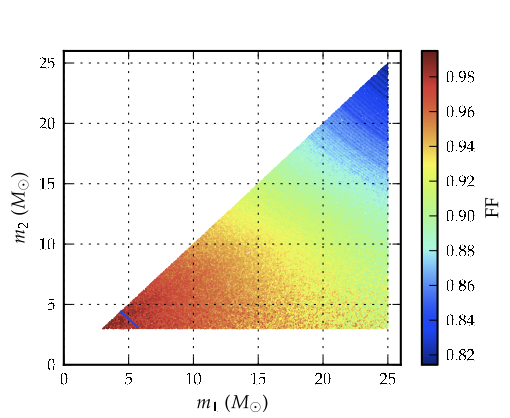
\includegraphics[scale=0.04, clip=false, totalheight=0.3\textheight, width=\columnwidth]{F2EOBeffectualness.pdf}
%\caption{\label{fig:match_f2eob_all}This figure shows the effectualness of a bank of Taylor F2 waveforms, with a minimal match of 0.97; at each point in the stellar-mass binary-black-hole region of the component-mass space. The color at each point is the maximum of overlap values between the full IMR EOB waveform for that point and the entire bank of Taylor F2 waveforms.}
%\end{figure}
%\begin{figure}
%\centering
%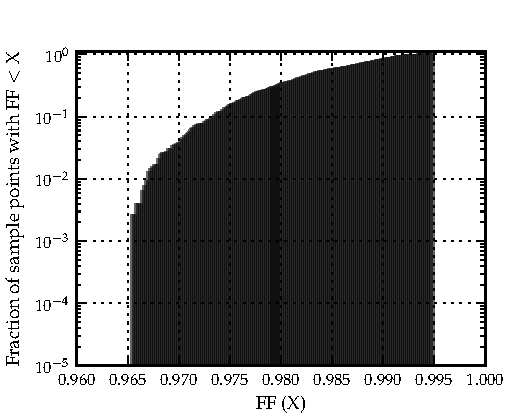
\includegraphics[scale=0.04, clip=false, totalheight=0.3\textheight, width=\columnwidth]{F2EOBhist.pdf}
%\caption{\label{fig:cumhist_f2eob_cut14}This figure shows a cumulative histogram of the fraction of the component-mass region, where the bank of Taylor F2 waveforms has an effectualness less than the respective values on the x-axis. For example, over $2\%$ of the component-mass region, the F2 bank has effectualness below $0.97$. The component-mass region shown here has systems with individual component-masses in $(3-20)M_{\odot}$ and total mass below or equal to $14M_{\odot}$.}
%\end{figure}
%\begin{figure*}[]
%\centerline{
%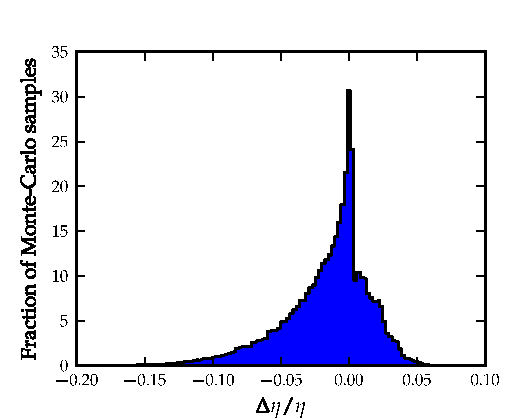
\includegraphics[scale=0.04, clip=false,keepaspectratio=true, width=\columnwidth]{hist_eta_err14paramF2EOB.pdf}\label{fig:errparams_f2eob_eta}              
%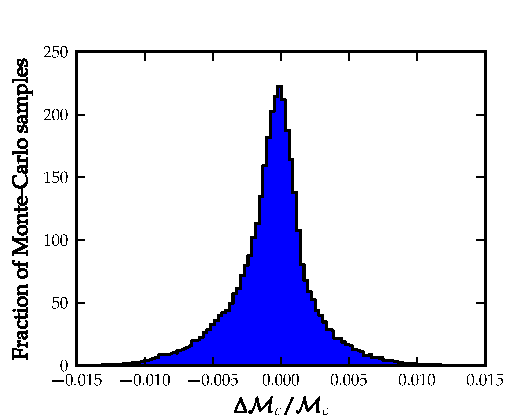
\includegraphics[scale=0.04, clip=false, keepaspectratio=true, width=\columnwidth]{hist_mchirp_err14paramF2EOB.pdf}\label{fig:errparams_f2eob_mchirp}
%}
%\caption{This figure shows the histogram of fractional difference between the physical parameters recovered by searching for the gravitational-wave signal using Taylor F2 bank of waveforms, and the actual physical parameters of the system used to generate the gravitational-wave signal. The left plot shows the fractional difference in the symmetric mass ratio $\eta$ and the right plot shows the fractional difference in the chirp mass $\mathcal{M}_c$. The designated component-mass-space region is the region with total mass below $14M_{\odot}$ and individual component-masses in $(3-20)M_{\odot}$.}
%\end{figure*}
%
%\begin{figure}
%\centering
%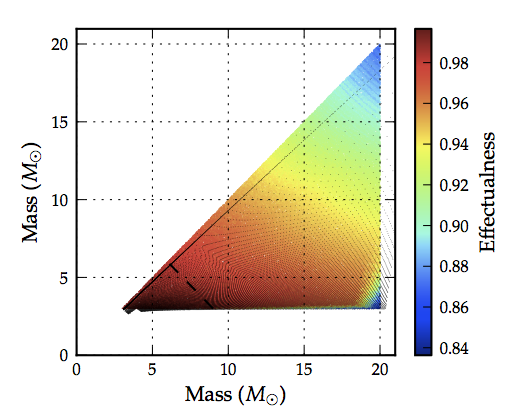
\includegraphics[scale=0.04, clip=false, totalheight=0.3\textheight, width=\columnwidth]{T4EOBeffectualness.pdf}
%\caption{\label{fig:match_t4eob_all}This figure shows the effectualness of a bank of Taylor T4 waveforms, with a minimal match of 0.97; at each point in the stellar-mass binary-black-hole region of the component-mass space. The color at each point is the maximum of overlap values between the full IMR EOB waveform for that point and the entire bank of Taylor T4 waveforms.}
%\end{figure}
%\begin{figure}
%\centering
%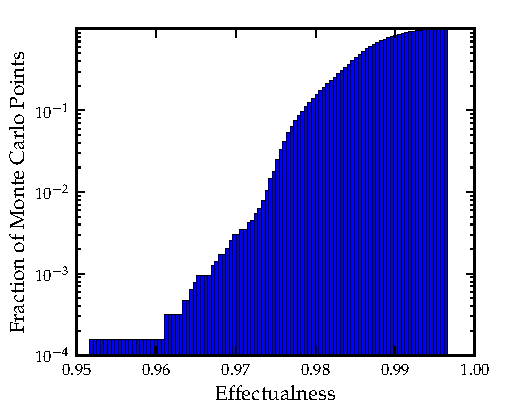
\includegraphics[scale=0.04, clip=false, totalheight=0.3\textheight, width=\columnwidth]{T4EOBhist.pdf}
%\caption{\label{fig:cumhist_t4eob_cut10}This figure shows a cumulative histogram of the fraction of the component-mass region, where the bank of Taylor T4 waveforms has an effectualness less than the respective values on the x-axis. For example, over $0.04\%$ of the component-mass region, the T4 bank has effectualness below $0.965$. The component-mass region shown here has systems with individual component-masses in $(3-20)M_{\odot}$ and total mass below or equal to $12M_{\odot}$.}
%\end{figure}
%\begin{figure*}[]
%\centerline{
%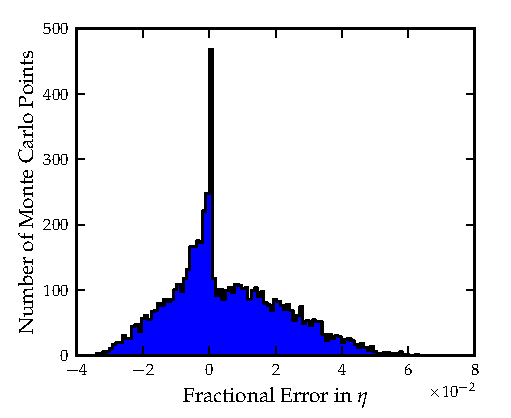
\includegraphics[scale=0.04, clip=false,keepaspectratio=true, width=\columnwidth]{hist_eta_err12paramT4EOB.pdf}\label{fig:errparams_t4eob_eta}              
%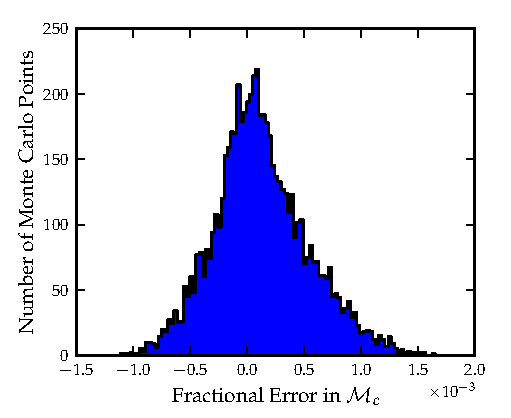
\includegraphics[scale=0.04, clip=false, keepaspectratio=true, width=\columnwidth]{hist_mchirp_err12paramT4EOB.pdf}\label{fig:errparams_t4eob_mchirp}
%}
%\caption{This figure shows the histogram of fractional difference between the physical parameters recovered by searching for the gravitational-wave signal using Taylor T4 bank of waveforms, and the actual physical parameters of the system used to generate the gravitational-wave signal. The left plot shows the fractional difference in the symmetric mass ratio $\eta$ and the right plot shows the fractional difference in the chirp mass $\mathcal{M}_c$. The designated component-mass-space region is the region with total mass below $12M_{\odot}$ and individual component-masses in $(3-20)M_{\odot}$.}
%\label{fig:errparams_t4eob}
%\end{figure*}
%
%Following the previous section, in this section we investigate in detail the region in the component-mass space where it suffices to use the PN approximants (Taylor F2 and T4) for matched-filtering detection searches, and where using EOB is clearly more viable. In this section, we address this question for searches that use a discrete \textit{bank} \citep{SathyaBankPlacementTauN,SathyaMetric2PN} of waveform templates, as were used in earlier searches done over the intial LIGO data \citep{Colaboration:2011nz,Abadie:2010yb,Abbott:2009qj,Abbott:2009tt,Messaritaki:2005wv}. As before, the region of the component-mass space that we study is the stellar-mass binary-black-hole region with individual component mass lying in $(3-20)M_{\odot}$.
%
%We do a Monte-Carlo simulation over the entire stellar-mass binary-black-hole mass region. The simulation was done by generating 100,000 points over the designated region of the component-mass space, uniformly distributed in individual component-mass. We take each of these points, and generate the full IMR EOB waveform for the system with component masses given by the coordinates of the point $a$, starting from the time when the gravitational-wave frequency from the system crosses 15Hz, and ending when the quasi-normal ringing of the final black-hole (formed by the coalescence of the binary) stops. Let $a$ represent a representative point and $h_a^{\EOB}$ be the EOB waveform (shown in superscript) for the point $a$ (shown in the subscript). We also generate a bank of template waveforms of approximant $\X$, using the Owen-Sathya bank placement metric \citep{OwenTemplateSpacing,SathyaBankPlacementTauN,SathyaMetric2PN} to cover the same mass region, with the requirement that the waveform generated for \textit{
%any} point $a$ in that mass-region will have a maximized overlap $\geq 0.97$ with \textit{at least} one point in the bank; i.e. $\Olap(h^{\X}_a,h^{\X}_b)\geq 0.97$ for at least one point $h^{\X}_b$ in the aforementioned bank of template waveforms . This is equivalent to saying that the bank has a \textit{minimal match} $\mathrm{MM}$ of $0.97$. Here, $\X$ could be either the Taylor F2 or Taylor T4 waveform approximant.
%
%Given a point $a$ in the component-mass space, and the exact waveform $h^e_a$ generated using the coordinates of the point $a$ as component-masses; the \textit{effectualness} of a bank of template waveforms (of approximant $\X$) is defined as the maximum value of maximized overlap between $h^e_a$ and any member $h^{\X}_b$ of the template waveform bank, i.e.
%\begin{equation}
%\mathcal{E}(h^e_a|h^{\X}) = \underset{b}{max}\dfrac{(h^e_a|h^{\X}_b)}{\sqrt{(h^e_a|h^e_a)(h^{\X}_b|h^{\X}_b)}}.
%\end{equation}
%When searching for signals in detector data, the data is matched-filtered through the entire bank of waveform templates and the maximum value of the SNR over the entire bank is used in further statistical analysis \citep{Colaboration:2011nz,Abadie:2010yb,Abbott:2009qj,Abbott:2009tt,Messaritaki:2005wv}. Thus, for a detection search that aims at less than $10\%$ loss in event detection rate, what is required is a bank of template waveforms that has effectualness above $0.965$ over the entire component-mass region that it covers \citep{WaveformAccuracy2008,WaveformAccuracy2010,CompTemplates2009}.
%
%In the Monte-Carlo simulation over the bank, for every point $a$ we approximate the exact $h^e_a$ with $h^{\EOB}_a$ \citep{EOBNRdevel01}, and calculate the effectualness of the template bank (generated for different waveform approximants) at each of the sample points distributed across the component-mass space.
%
%\subsection{TaylorF2}\label{sec:level2:EffectualnessTaylorF2}
%Fig.~\ref{fig:match_f2eob_all} shows the effectualness of the Taylor F2 template bank at each point in the component-mass space. We observe a region of the component-mass space where the effectualness of the bank is high enough to not have an event detection rate loss above $10\%$, which corresponds to a minimal effectualness of $0.965$ \citep{WaveformAccuracy2008,WaveformAccuracy2010}. Looking in detail at the region of the space with total-masses below $14M_{\odot}$, we see that in this region of the component-mass space, the bank of Taylor F2 waveform templates has effectualness greater than $0.965$ throughout. This is illustrated by the histogram in Fig.~\ref{fig:cumhist_f2eob_cut14}. This cumulative histogram shows the relative fraction of the component-mass-space region (with total mass below $14M_{\odot}$) over which the Taylor F2 waveform template bank has an effectualness below or equal to the value on the x-axis. As can be seen, the Taylor F2 bank has, at all the points sampled in this region, 
%effectualness above $0.965$. This corresponds to a maximum loss in event rate of $10\%$ \citep{WaveformAccuracy2008,WaveformAccuracy2010}.
%
%Also, in Fig.~\ref{fig:errparams_f2eob}, we can see a histogram of the fractional differences between the true physical mass parameters of a system and the mass parameters of the template waveform in the Taylor F2 bank that has the maximum value of maximized overlap with the IMR EOB waveform for that system. In other words, it shows the fractional error in the mass parameters recovered using a bank of F2 waveform templates. The mass-coordinates we show the errors in are the dimensionless symmetric mass-ratio $\eta$, and the chirp mass $\mathcal{M}_c$,
%\begin{equation}
%\mathcal{M}_c = M \eta^{3/5}.
%\end{equation}
%This chirp mass parameter determines the total length in time of the inspiral part of the waveform (to leading order) \citep{SathyaBankPlacementTauN}, and it contains more information than the component-mass parameters. This is also the reason why the chirp mass is recovered with greater precision, as seen in Fig.~\ref{fig:errparams_f2eob}. This illustrates that there are no accidental matches of the IMR EOB and Taylor F2 waveforms with very different physical parameters, as the fractional difference between the actual physical parameters of the system and those recovered using the Taylor F2 template bank are $\lesssim 6\%$ for $\eta$ and $\lesssim 0.15\%$ for chirp mass, which are within the expected range [citation].
%
%\subsection{TaylorT4}\label{sec:level2:EffectualnessTaylorT4}
%Fig.~\ref{fig:match_t4eob_all} shows the effectualness of the Taylor T4 template bank at each point in the component-mass space. As with the Taylor F2 case, we observe a region of the component-mass space where the effectualness of the bank is above the acceptable minimum of $0.965$ \citep{WaveformAccuracy2008,WaveformAccuracy2010}. We found, looking in detail at the region of the space with total-masses below $12M_{\odot}$, that in this region of the component-mass space, the Taylor T4 template bank has effectualness above $0.965$ over more than $99.9\%$ of the region. This is illustrated in Fig.~\ref{fig:cumhist_t4eob_cut12}, which shows the fraction of the component-mass region (with total mass below $12M_{\odot}$) where the T4 template bank has an effectualness below the corresponding number on the x-axis. The histogram shows that, over no more than $0.02\%$ of the component-mass area does the effectualness of the T4 template bank drop below $0.965$.
%
%As before, in Fig.~\ref{fig:errparams_t4eob}, we show a histogram of the fractional differences between the true physical parameters of a system and the parameters of the template in the Taylor T4 bank that has the maximum value of maximized overlap with the IMR EOB waveform for that system.
%This illustrates that there are no accidental matches of the IMR EOB and Taylor T4 waveforms with very different physical parameters, as the fractional difference between the actual physical parameters of the system and those recovered using the Taylor F2 template bank, which are $\lesssim 4\%$ for $\eta$ and $\lesssim 0.1\%$ for chirp mass, are within expected bounds [citation].
%
% If you have acknowledgments, this puts in the proper section head.
\begin{acknowledgments}
The authors are thankful to Ian Harry, Eliu Huerta, and the Syracuse GW group for fruitful discussions. This work was supported NSF grants PHY-0847611 and PHY-0854812. Computations were carried out on the SUGAR cluster which is supported by NSF grants PHY-1040231, PHY-1104371, and PHY-0600953, and by Syracuse University ITS.
\end{acknowledgments}

% Create the reference section using BibTeX:
\bibliography{bank_effectualness_study}

\end{document}
%
% ****** End of file apstemplate.tex ******

